\chapter{Risultati Sperimentali}
\label{cap:RisultatiSperimentali}

\emph{Questo capitolo valuta sperimentalmente l'estensione carbon-aware
di Serverledge proposta in questa tesi. La valutazione non mira a
dimostrare una riduzione generalizzata del consumo energetico: il consumo
è considerato una dimensione del trade-off con la qualità del risultato,
da modulare in funzione del contesto carbonico dell'esecuzione.
L'obiettivo è verificare che lo scheduler carbon-aware traduca la carbon
intensity della zona in scelte coerenti lungo la frontiera di Pareto:
privilegiare varianti più efficienti quando il costo carbonico
dell'energia è elevato, mantenere varianti più accurate quando tale costo
è ridotto.}

% -----------------------------------------------------------
\section{Setup sperimentale}
\label{sec:setup-sperimentale}
% -----------------------------------------------------------

La valutazione è stata condotta su un'installazione di Serverledge estesa
con i componenti descritti nei Capitoli~\ref{cap:ProgettazioneRealizzazione}
e~\ref{cap:scheduler}. L'ambiente è composto da tre macchine virtuali
ospitate su una macchina fisica equipaggiata con processore Intel Core
i5-12400, tutte eseguite su Ubuntu Server 22.04 LTS. La prima macchina
virtuale (4~vCPU, 12~GB RAM) ospita il nodo Serverledge insieme all'intero
stack di monitoraggio e al registro delle varianti in \texttt{etcd}. La
seconda (2~vCPU, 4~GB RAM) è dedicata alla generazione del carico, tramite
la CLI di Serverledge e gli script di benchmark. La terza (2~vCPU, 4~GB RAM)
esegue InfluxDB, separata dal nodo principale per evitare contesa sulle
risorse durante la raccolta delle metriche.

% -----------------------------------------------------------
\subsection{Funzioni utilizzate}
\label{subsec:funzioni-utilizzate}
% -----------------------------------------------------------

Le funzioni usate negli esperimenti coprono due famiglie applicative:
\emph{funzioni numeriche} e \emph{funzioni di classificazione} (ML).
Questa scelta consente di valutare lo scheduler su due modalità di
approssimazione strutturalmente diverse, con implicazioni distinte sul
comportamento della frontiera di Pareto.

\paragraph{Funzioni numeriche.}
Le tre funzioni numeriche calcolano grandezze matematiche note tramite
serie o metodi iterativi, e la qualità è misurata come errore relativo
rispetto al valore esatto. \emph{PiLeibniz} approssima $\pi$ mediante la
serie di Leibniz troncata a un numero variabile di termini; le varianti si
distinguono per il numero di iterazioni e per il linguaggio di
implementazione (Python e C). \emph{LnHarmonic} stima $\ln 2$ tramite la
serie armonica alternata, con un insieme analogo di varianti a granularità
crescente. \emph{MonteCarlo} stima $\pi$ tramite campionamento casuale;
in questo caso l'intervallo energetico tra varianti è particolarmente
ampio ($1575\times$), poiché il numero di campioni varia su più ordini
di grandezza.

\paragraph{Funzioni di classificazione.}
Le tre funzioni ML eseguono compiti di classificazione su testo o immagini,
e la qualità è espressa come \texttt{quality\_score} normalizzato in
$[0,1]$, derivato dall'accuratezza del modello sul dataset di riferimento.
\emph{SentimentAnalysis} classifica il tono di un testo e dispone di
quattro modelli: RoBERTa-large, DistilBERT, BERT-tiny e VADER,
classificatore a dizionario privo di inferenza neurale.
\emph{SpamDetection} individua messaggi indesiderati con un'architettura
analoga, con RoBERTa-spam come variante di riferimento e un classificatore
a parole chiave come variante minima. \emph{ImageClassification} classifica
immagini su 1000 categorie ImageNet tramite quattro architetture: ViT-Base,
EfficientNet-B0, MobileNet-V2 e MobileNet-V2-Tiny.

Nelle funzioni numeriche la relazione tra numero di iterazioni ed errore
è continua: la frontiera di Pareto è densa e lo scheduler può modulare
il compromesso energia--qualità in modo graduale. Nelle funzioni ML,
invece, ogni variante corrisponde a un modello architetturalmente distinto:
la frontiera è composta da pochi punti discreti e il passaggio a una
variante più leggera può comportare un salto qualitativo più marcato.
Questa differenza strutturale si riflette direttamente nelle scelte dello
scheduler e sarà visibile nei risultati sperimentali.

La Tabella~\ref{tab:funzioni-varianti} riassume il numero di varianti
disponibili e l'intervallo di energia di invocazione per ciascuna
funzione. Le Figure~\ref{fig:pileibniz-energy-error}
e~\ref{fig:sentiment-energy-quality} mostrano due casi rappresentativi,
uno per famiglia, mettendo in relazione il costo energetico con la misura
di qualità usata dallo scheduler. A partire da questi profili, la
frontiera di Pareto e le soglie di selezione lungo l'asse $\lambda$ sono
proprietà della funzione e delle sue varianti, indipendenti dallo specifico
esperimento. Ciò che cambia tra gli esperimenti è il modo in cui la carbon
intensity viene trasformata nel valore corrente di $\lambda$, e quindi la
regione della frontiera effettivamente attraversata durante l'esecuzione.

\begin{table}[H]
    \centering
    \caption{Funzioni utilizzate nella valutazione sperimentale e profili
             energetici iniziali delle varianti.}
    \label{tab:funzioni-varianti}
    \begin{tabular}{llrrr}
        \toprule
        Funzione & Famiglia & Varianti & $E_{\min}$ (J) & $E_{\max}$ (J) \\
        \midrule
        PiLeibniz           & Numerica & 9 & 0.000196 & 0.007823 \\
        LnHarmonic          & Numerica & 7 & 0.000196 & 0.007700 \\
        MonteCarlo          & Numerica & 6 & 0.000147 & 0.231480 \\
        SentimentAnalysis   & ML       & 4 & 0.002400 & 0.091579 \\
        SpamDetection       & ML       & 4 & 0.002000 & 0.085000 \\
        ImageClassification & ML       & 4 & 0.077000 & 1.455263 \\
        \bottomrule
    \end{tabular}
\end{table}

\begin{figure}[H]
    \centering
    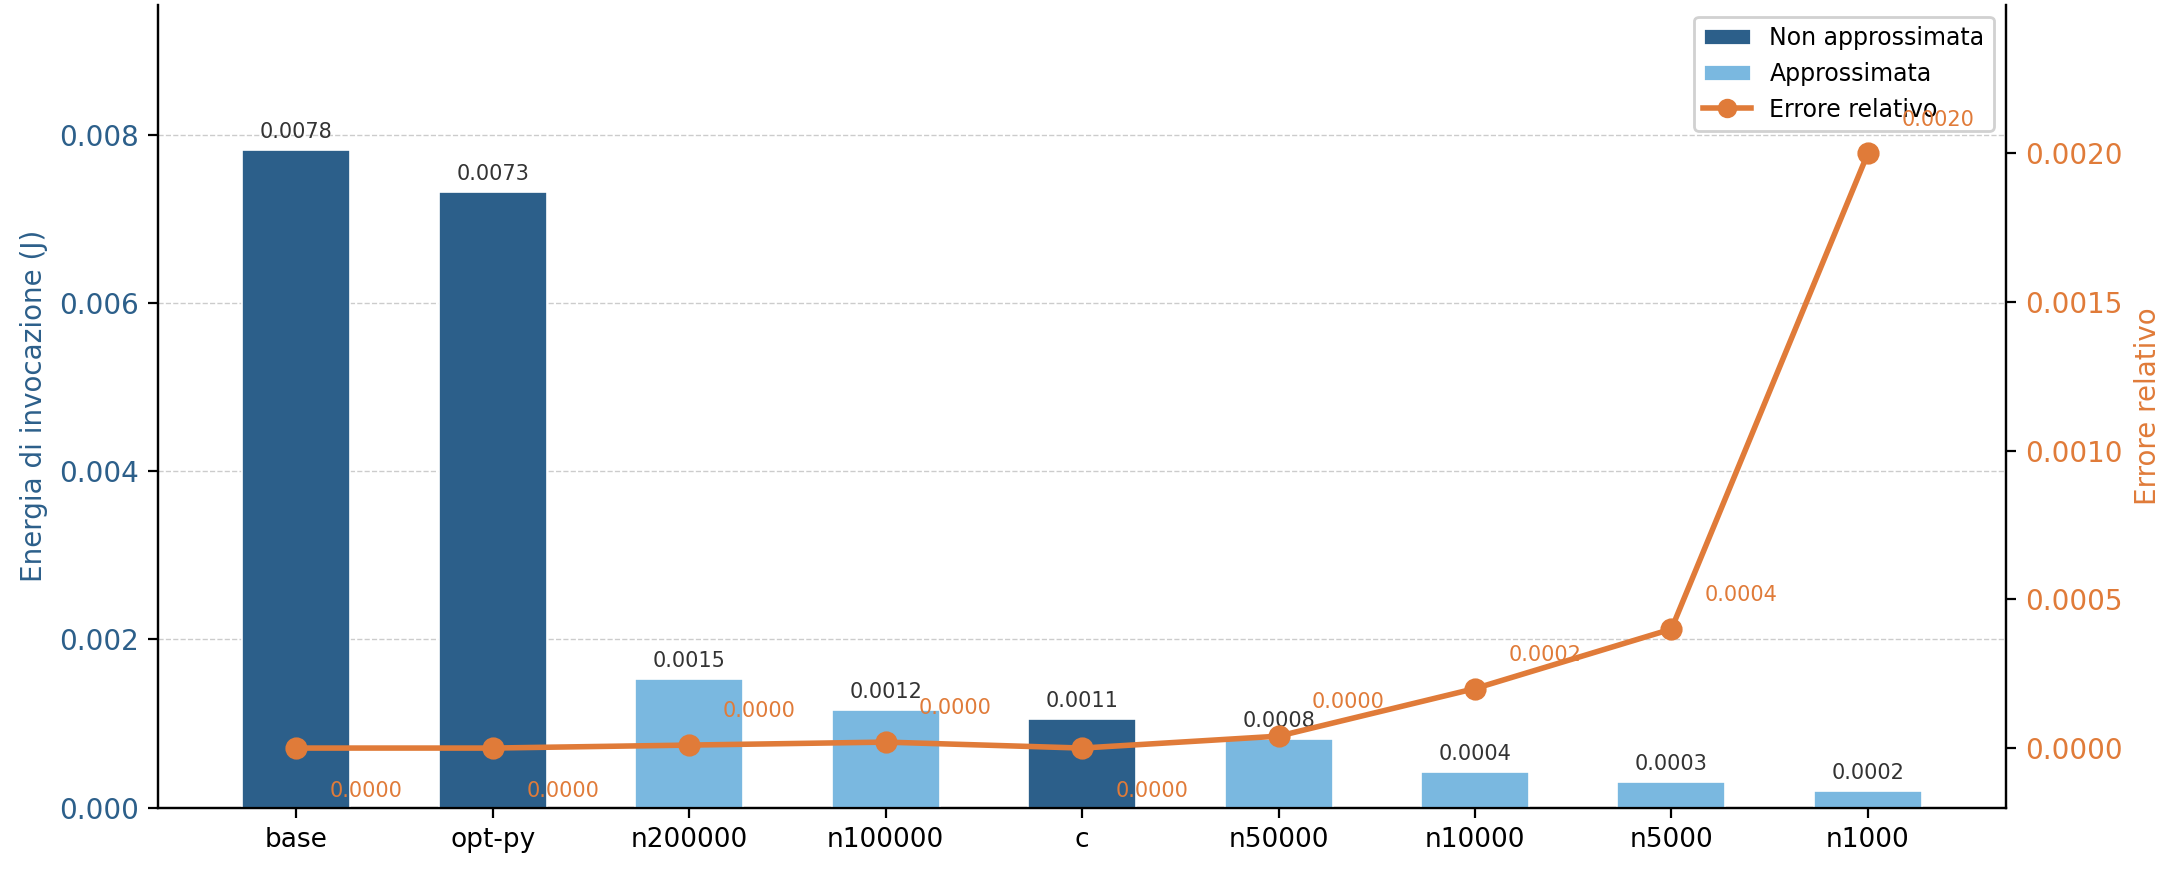
\includegraphics[width=0.98\textwidth]{figures/validation/pileibniz_v2.png}
    \caption{Energia di invocazione ed errore relativo delle varianti di
             PiLeibniz in scenario warm. Le varianti esatte presentano
             errore nullo, mentre le varianti approssimate riducono
             progressivamente l'energia diminuendo il numero di termini
             della serie. L'errore resta contenuto per le varianti
             intermedie e cresce solo per le approssimazioni più spinte,
             evidenziando una frontiera energia--accuratezza densa e
             modulabile.}
    \label{fig:pileibniz-energy-error}
\end{figure}

\begin{figure}[H]
    \centering
    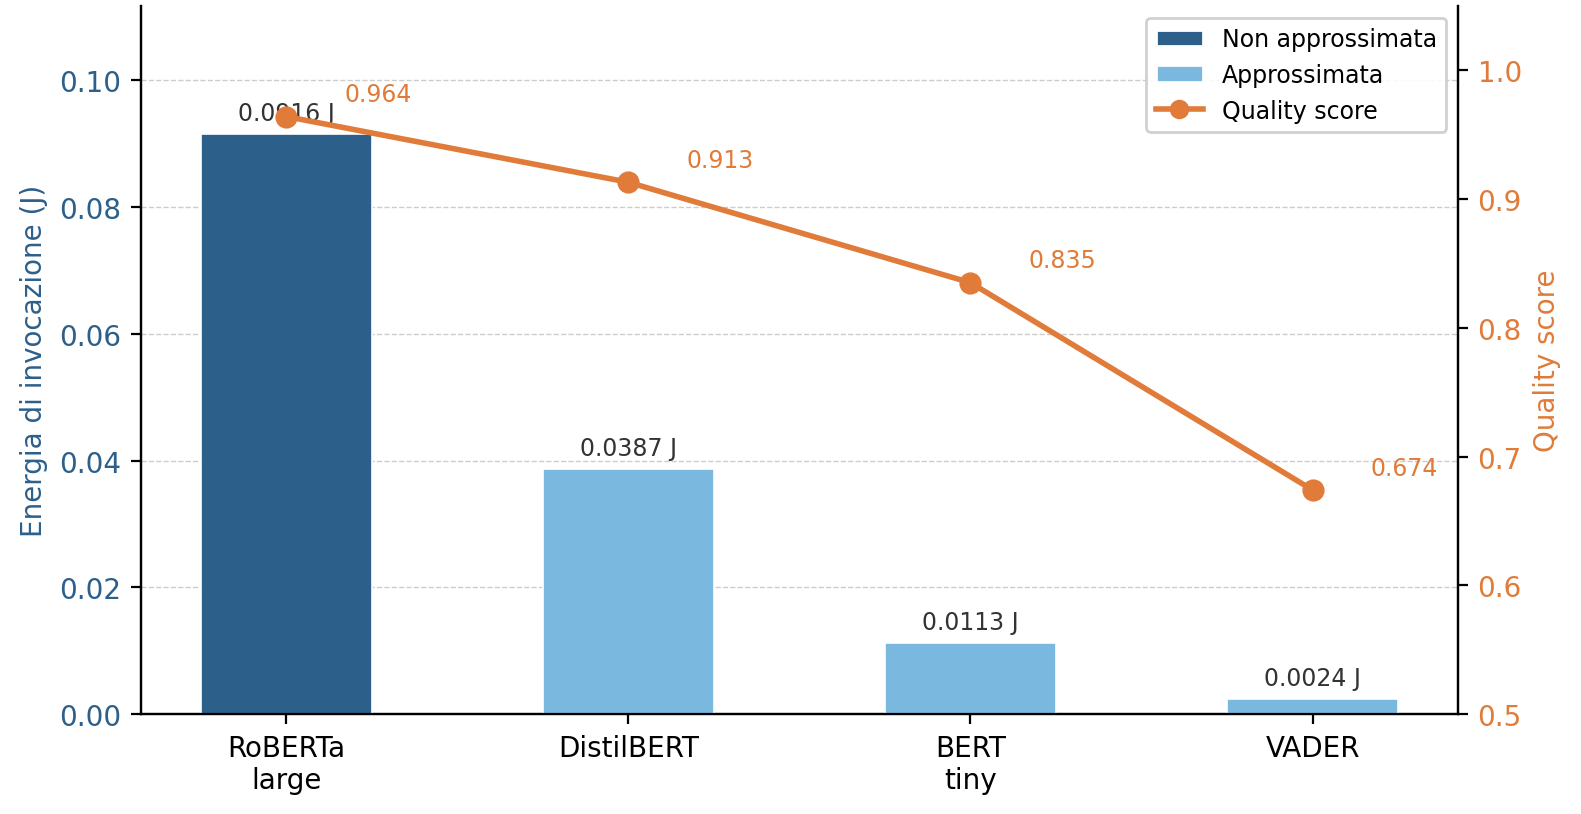
\includegraphics[width=0.90\textwidth]{figures/validation/sa_full.png}
    \caption{Energia di invocazione e \texttt{quality\_score} delle
             varianti di SentimentAnalysis. Il passaggio a modelli più
             leggeri riduce sensibilmente il costo energetico, ma la
             qualità diminuisce per salti discreti, riflettendo la natura
             architetturalmente distinta delle varianti ML.}
    \label{fig:sentiment-energy-quality}
\end{figure}

\begin{figure}[H]
    \centering
    \begin{subfigure}{0.98\textwidth}
        \centering
        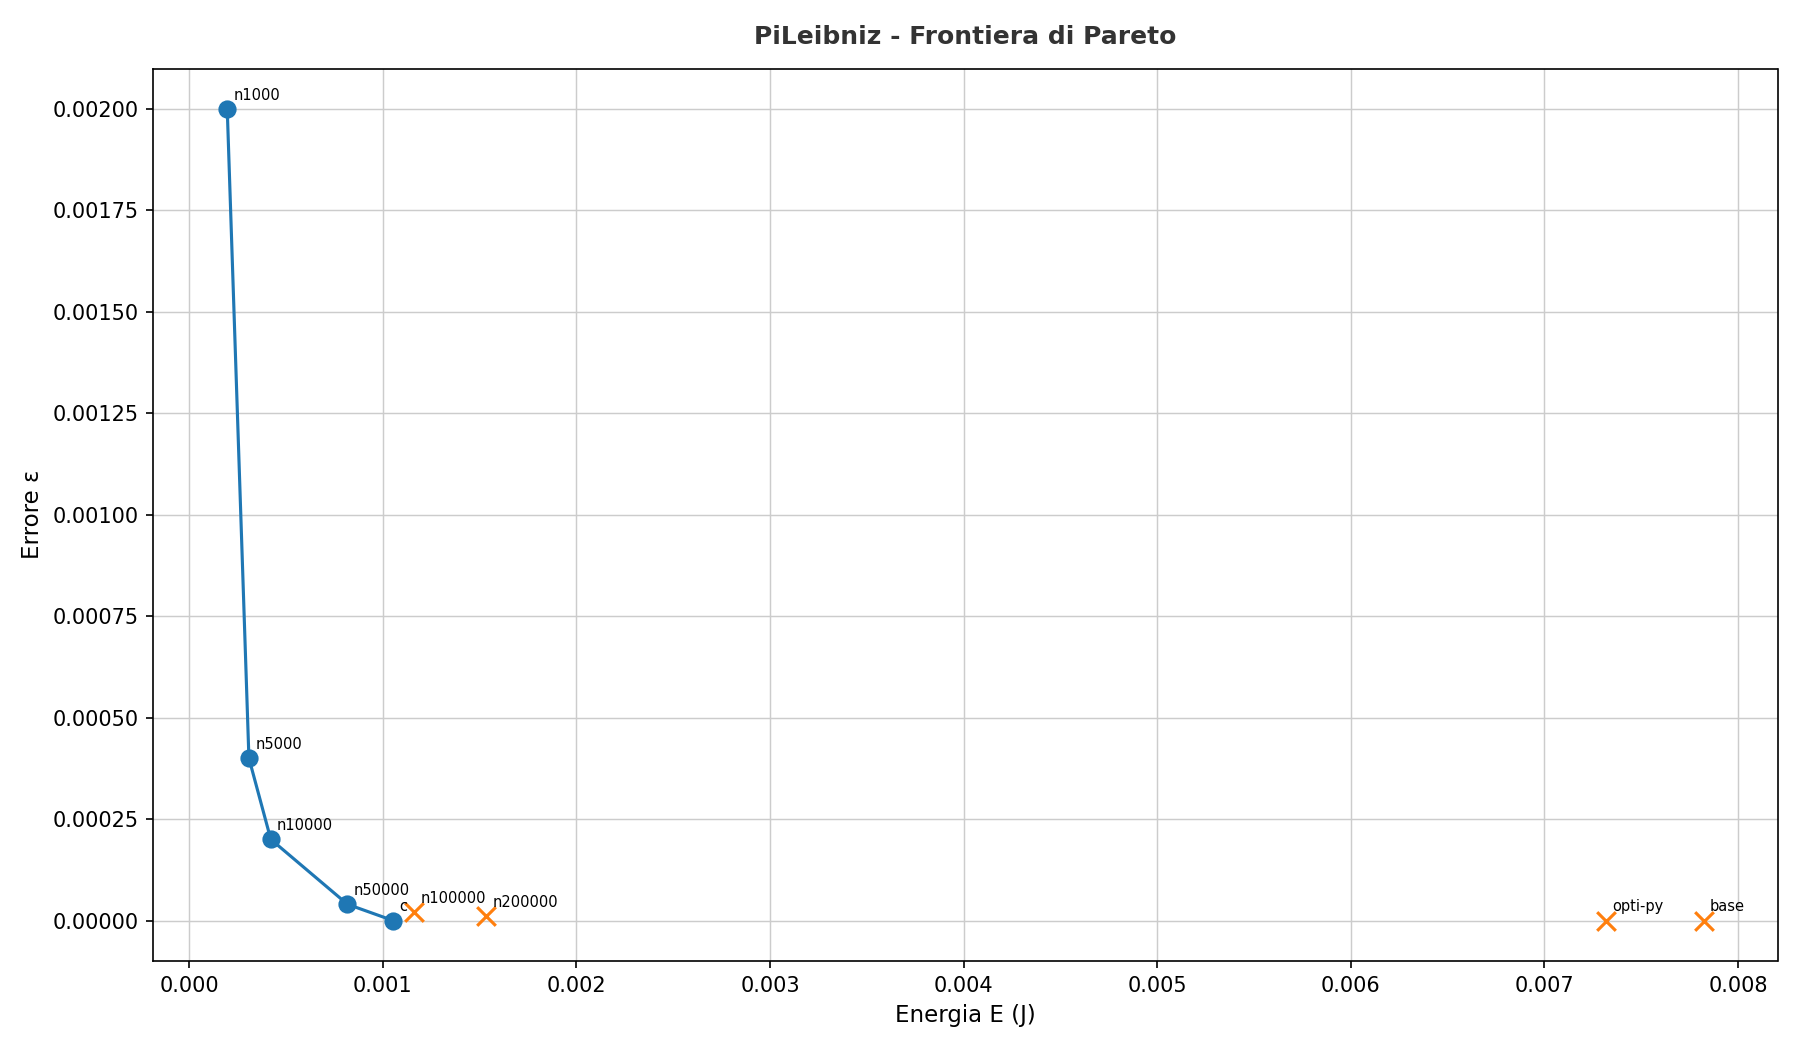
\includegraphics[width=\textwidth]{figures/validation/PiLeibniz-ParetoSetup.png}
        \caption{PiLeibniz}
    \end{subfigure}
    \vspace{0.4cm}
    \begin{subfigure}{0.98\textwidth}
        \centering
        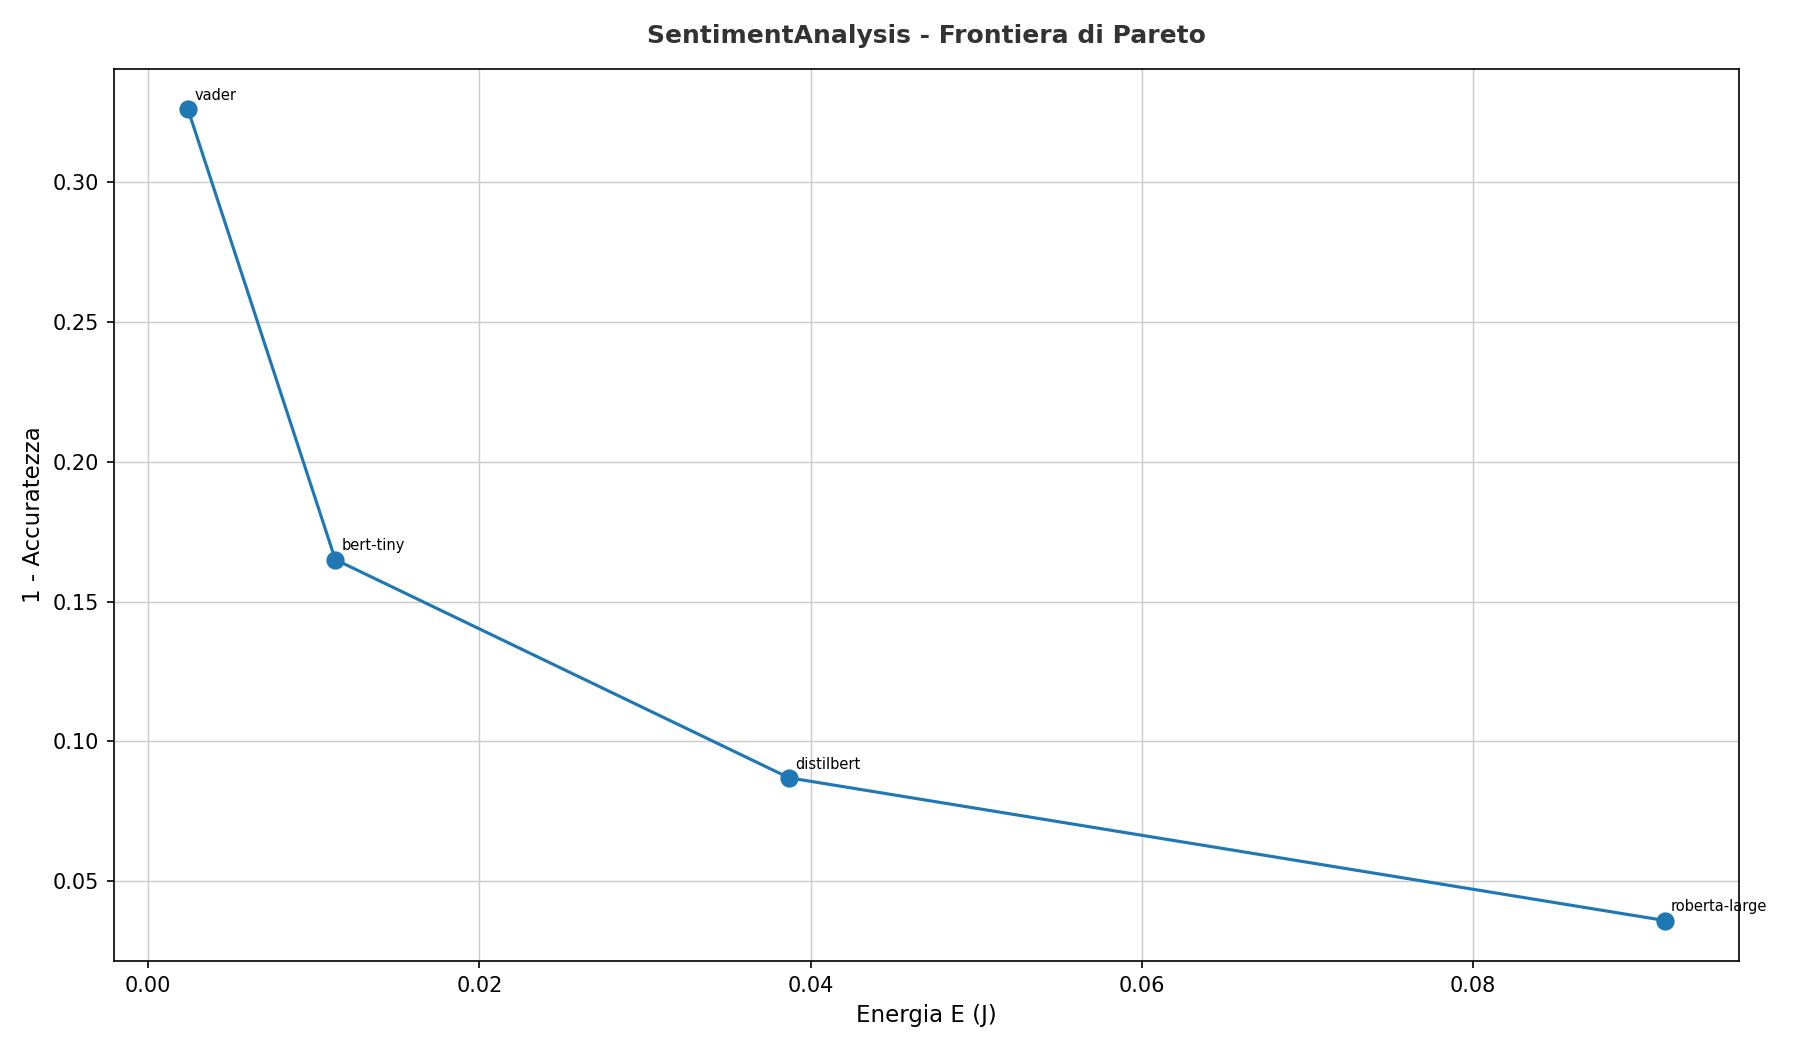
\includegraphics[width=\textwidth]{figures/validation/SentimentAnalysis-ParetoSetup.png}
        \caption{SentimentAnalysis}
    \end{subfigure}
    \caption{Frontiere di Pareto per le due funzioni rappresentative.
             Le varianti dominate non vengono considerate dallo scheduler;
             i punti non dominati definiscono i soli candidati selezionabili
             tramite scalarizzazione.}
    \label{fig:pareto-setup}
\end{figure}

\begin{figure}[H]
    \centering
    \begin{subfigure}{0.98\textwidth}
        \centering
        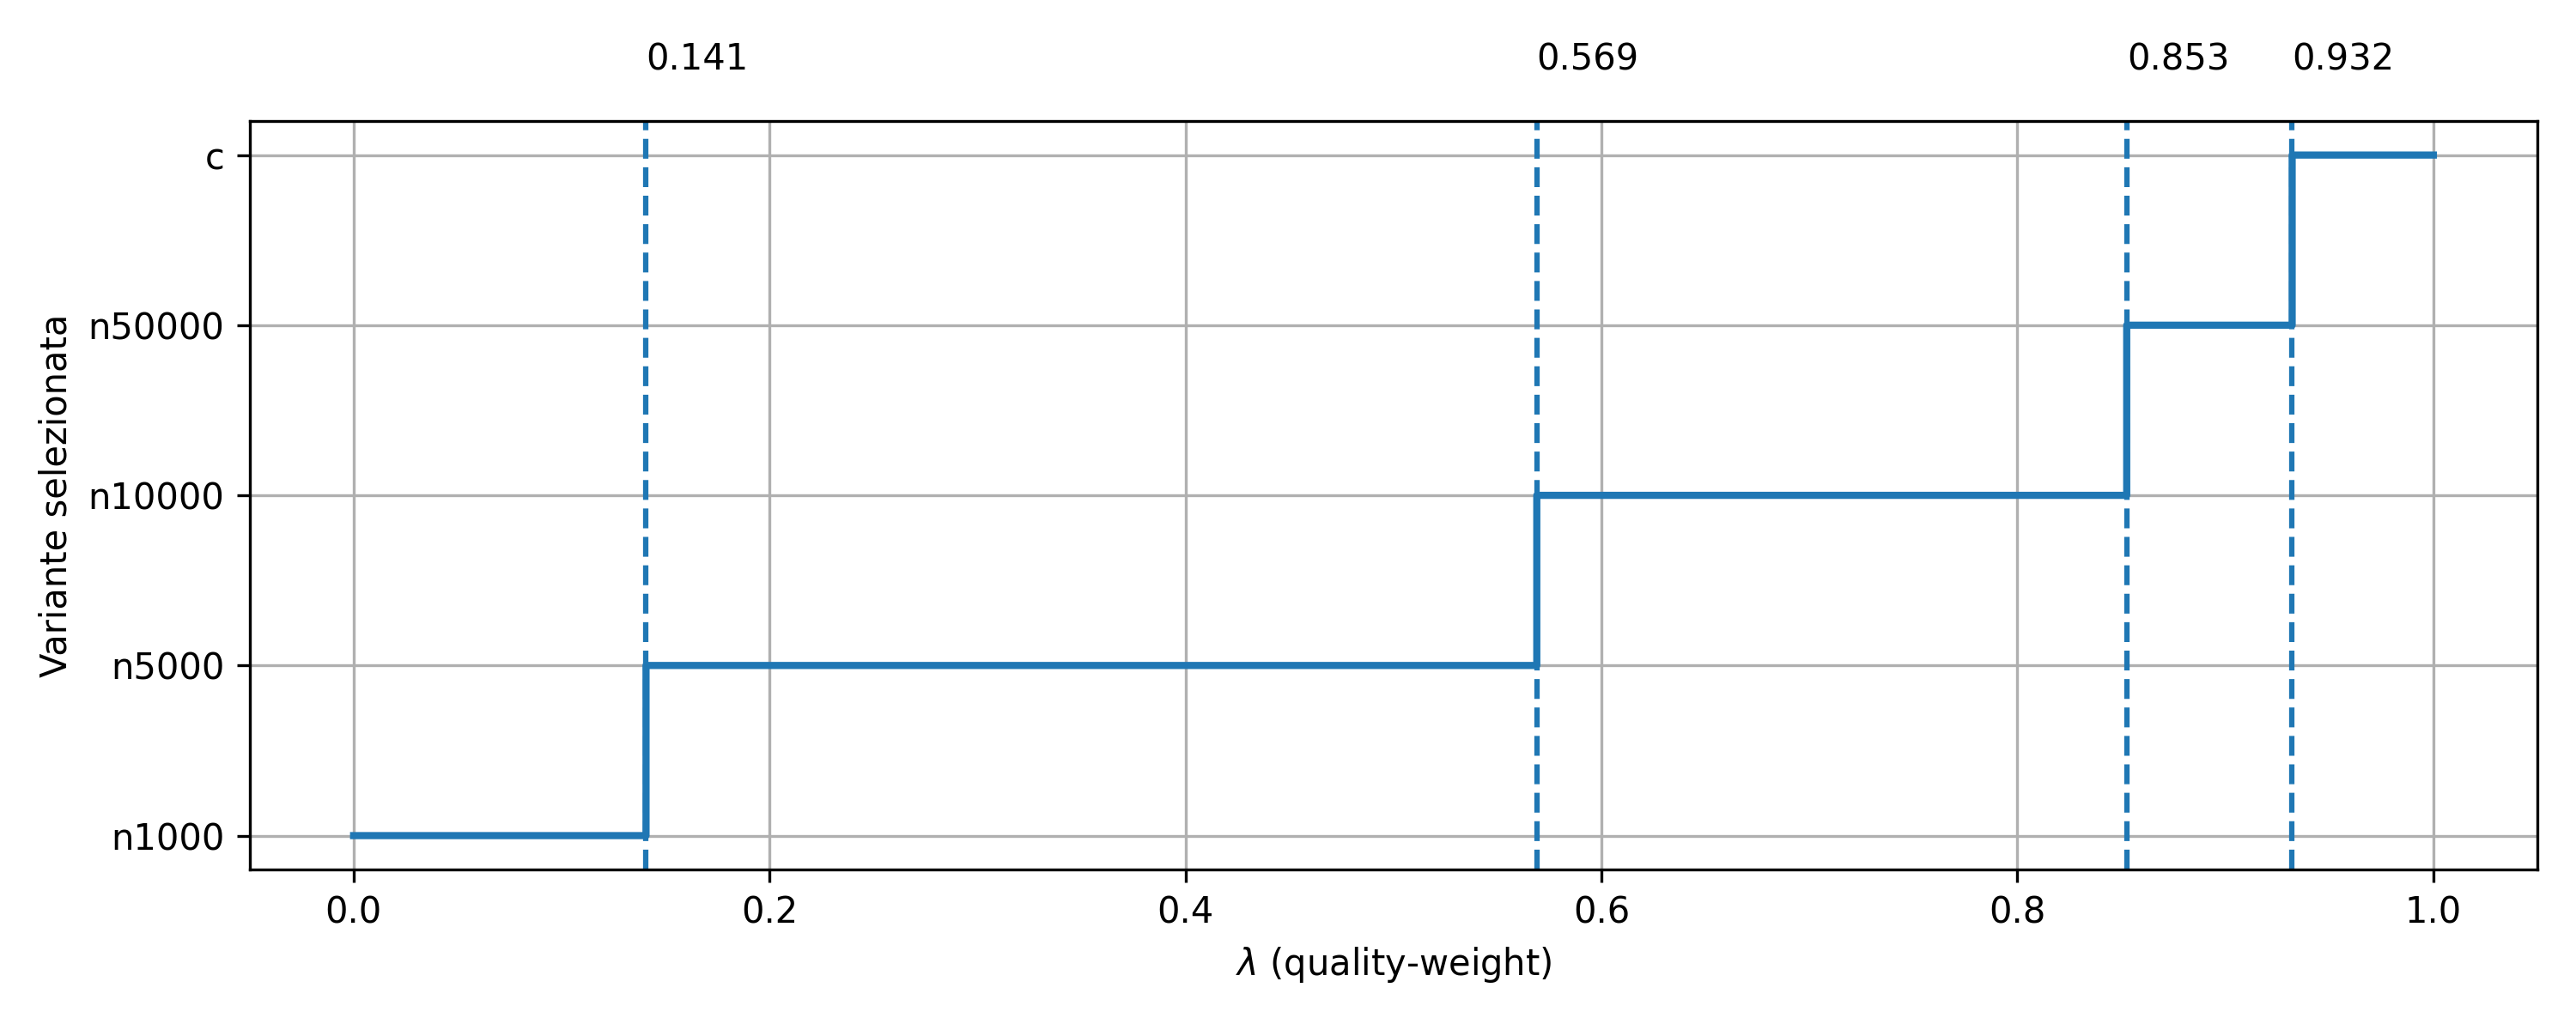
\includegraphics[width=\textwidth]{figures/validation/PiLeibniz-LambdaToVariant.png}
        \caption{PiLeibniz}
    \end{subfigure}
    \vspace{0.4cm}
    \begin{subfigure}{0.98\textwidth}
        \centering
        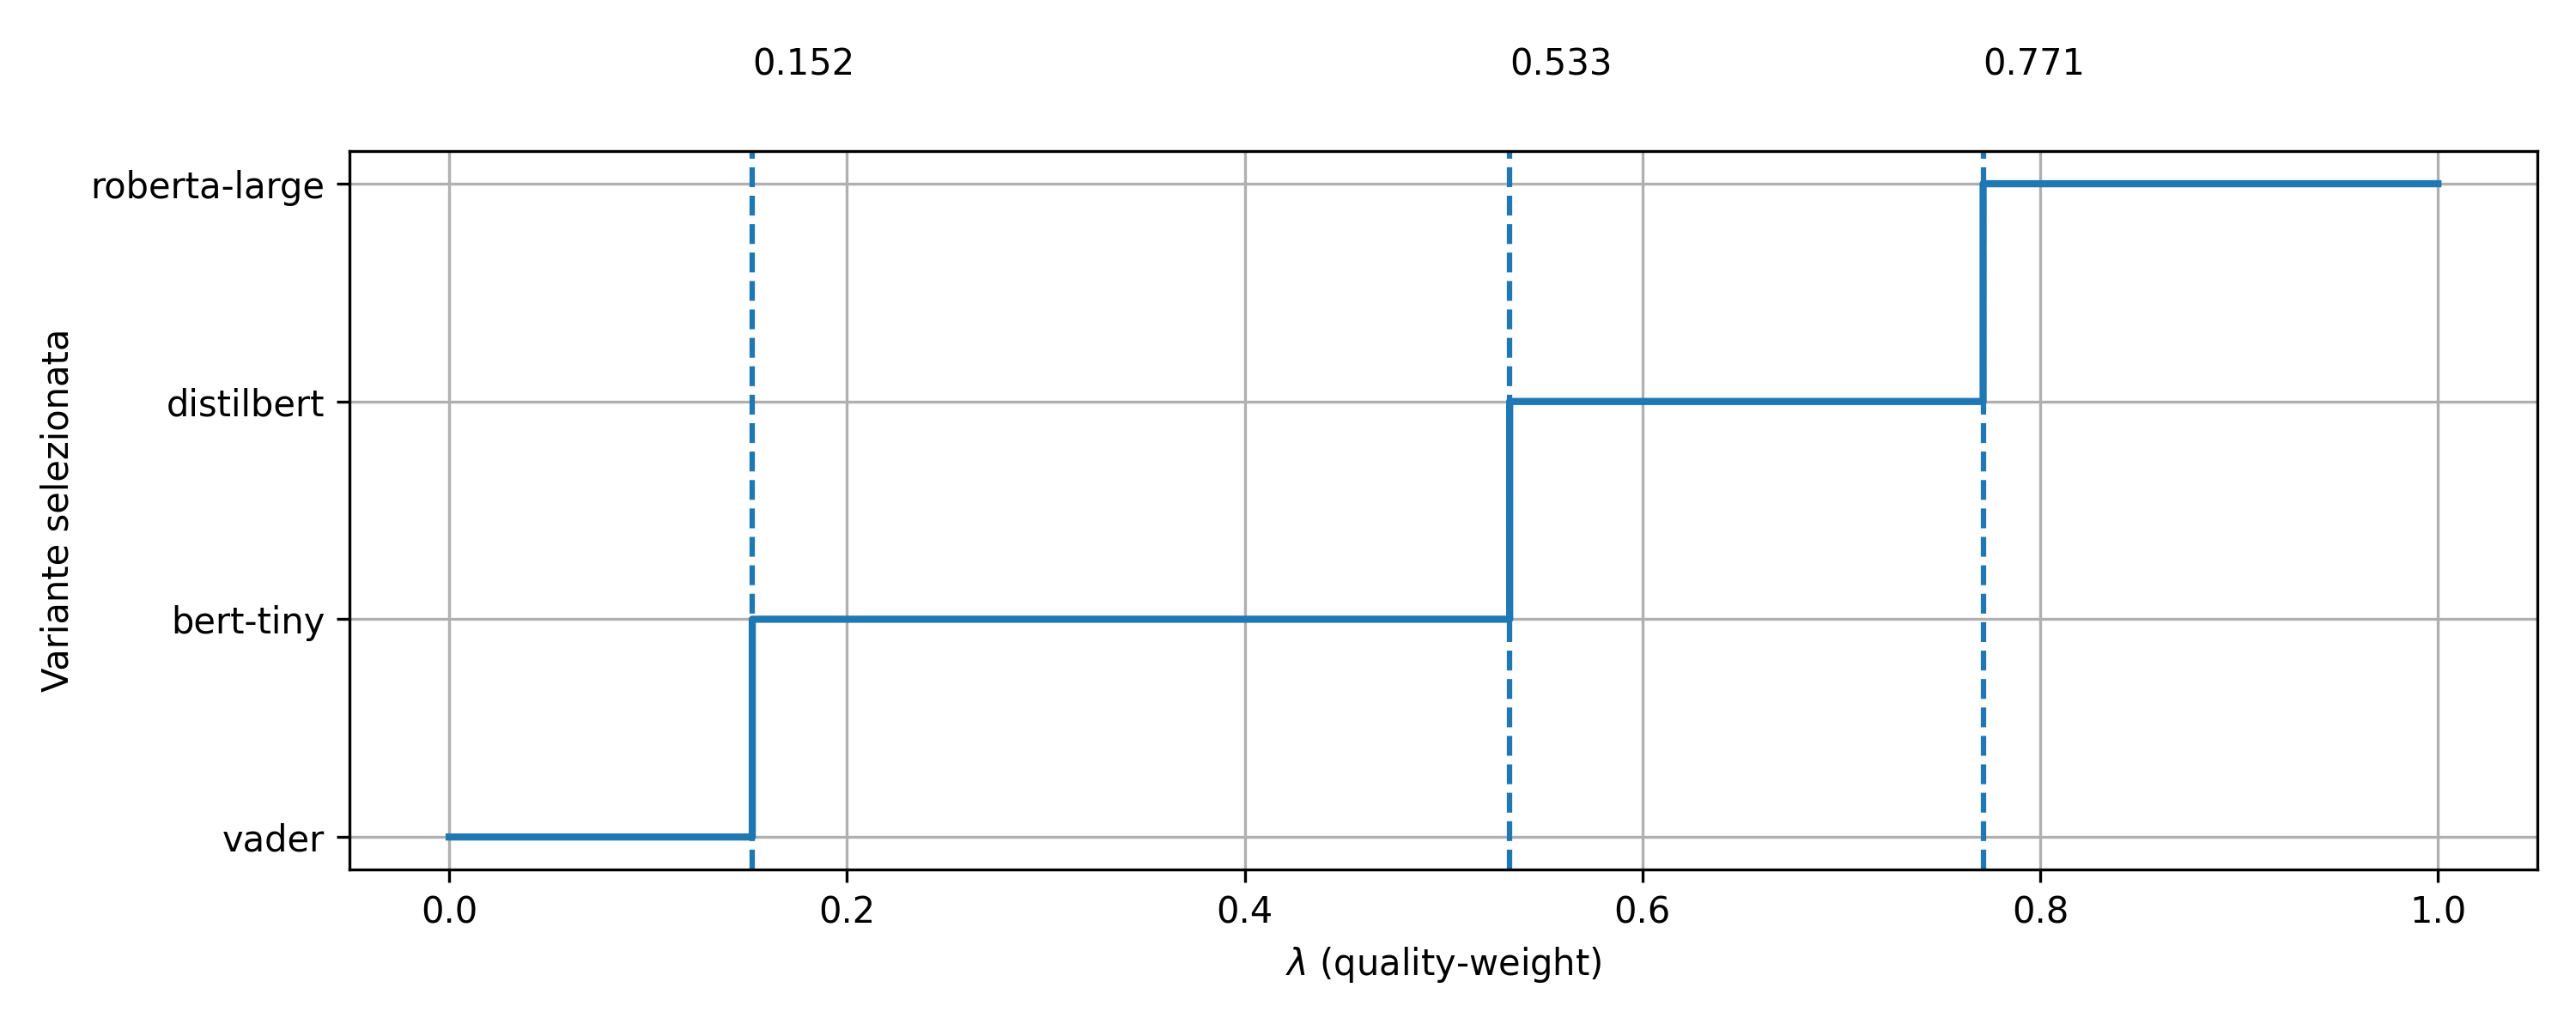
\includegraphics[width=\textwidth]{figures/validation/SentimentAnalysis-LambdaToVariant.png}
        \caption{SentimentAnalysis}
    \end{subfigure}
    \caption{Regioni di selezione delle varianti al variare di $\lambda$.
             Le soglie verticali derivano dai profili energia--qualità delle
             varianti Pareto-ottimali; nei diversi esperimenti cambia la
             traiettoria dei valori di $\lambda$, non questa mappa di
             selezione.}
    \label{fig:lambda-to-variant-setup}
\end{figure}

% -----------------------------------------------------------
\subsection{Strategie di confronto}
\label{subsec:strategie-confronto}
% -----------------------------------------------------------

In tutti gli esperimenti vengono confrontate tre strategie. La prima,
\emph{always-accurate}, rappresenta il comportamento legacy della
piattaforma: viene selezionata sempre la variante con errore minimo o
qualità massima, indipendentemente dalle condizioni ambientali. La seconda,
\emph{always-energy}, seleziona sempre la variante con minore energia di
invocazione, senza considerare la qualità del risultato; questa politica
non costituisce un caso operativo realistico, ma fornisce il limite
inferiore del consumo ottenibile con il modello di varianti adottato. La
terza è lo scheduler carbon-aware oggetto di questa tesi: quando l'utente
autorizza l'uso di varianti approssimate tramite il parametro
\texttt{AllowApprox=true}, il sistema costruisce la frontiera di Pareto
nello spazio energia--qualità e seleziona la variante in base alla
scalarizzazione descritta nel Capitolo~\ref{cap:scheduler}.

Il parametro $\lambda \in [0,1]$ regola il peso relativo tra qualità del
risultato e risparmio energetico: valori elevati di $\lambda$ privilegiano
la qualità, valori ridotti favoriscono l'efficienza energetica. Il valore
di $\lambda$ è derivato dalla carbon intensity (CI) della zona di esecuzione
tramite una funzione sigmoidale, garantendo che la selezione della variante
sia contestuale all'impatto carbonico dell'energia disponibile.

% -----------------------------------------------------------
\section{Protocollo di valutazione}
\label{sec:protocollo-valutazione}
% -----------------------------------------------------------

Gli Esperimenti~1 e~2 sono condotti a tempo discreto: per ciascuna zona
viene riletta una traccia di invocazioni da file e ogni richiesta viene
valutata rispetto alla CI associata al passo temporale corrente, estratta
dalle serie storiche orarie di ElectricityMaps~\cite{electricitymaps2024}.
Questo approccio isola il comportamento decisionale dello scheduler da
eventuali variazioni del carico e consente di confrontare due diverse
calibrazioni del segnale carbon-aware. L'Esperimento~1 mantiene fissa la
funzione sigmoide per tutte le zone: le tracce di CI restano diverse, ma
vengono trasformate in $\lambda$ tramite la stessa mappa decisionale.
L'Esperimento~2 utilizza invece una calibrazione locale, più aderente a un
deployment reale, in cui la CI corrente viene interpretata rispetto alla
distribuzione storica della zona. L'Esperimento~3 adotta infine un modello
a tempo continuo, con richieste che arrivano secondo un profilo di carico
variabile, al fine di valutare la stabilità del sistema e l'overhead della
selezione a runtime.

\paragraph{Zone considerate.}
Le zone geografiche considerate in tutti gli esperimenti sono Francia (FR),
Spagna (ES), Italia (IT), Germania (DE) e Polonia (PL), ordinate per CI
media crescente. La scelta copre un intervallo ampio e rappresentativo del
panorama europeo: la Francia rappresenta un regime a bassa CI (prevalente
energia nucleare), la Polonia un regime ad alta CI (prevalente energia da
carbone), mentre Spagna, Italia e Germania occupano fasce intermedie con
mix energetici diversificati. La Tabella~\ref{tab:ci-zone} riporta le
statistiche sintetiche della traccia impiegata, mentre la
Figura~\ref{fig:ci-distribution-zone} ne mostra la distribuzione per zona.

\begin{table}[H]
    \centering
    \caption{Statistiche della carbon intensity nelle zone considerate.}
    \label{tab:ci-zone}
    \resizebox{\textwidth}{!}{%
    \begin{tabular}{lrrrr}
        \toprule
        Zona    & CI media (g/kWh) & CI minima (g/kWh) & CI massima (g/kWh)\\
        \midrule
        Francia  &  14.8 &   2.4 &  64.3 \\
        Spagna   &  91.3 &  30.8 & 260.9 \\
        Italia   & 197.4 &  60.0 & 332.3 \\
        Germania & 279.2 &  72.1 & 566.7 \\
        Polonia  & 519.3 & 249.6 & 728.4 \\
        \bottomrule
    \end{tabular}
    }
\end{table}

\begin{figure}[H]
    \centering
    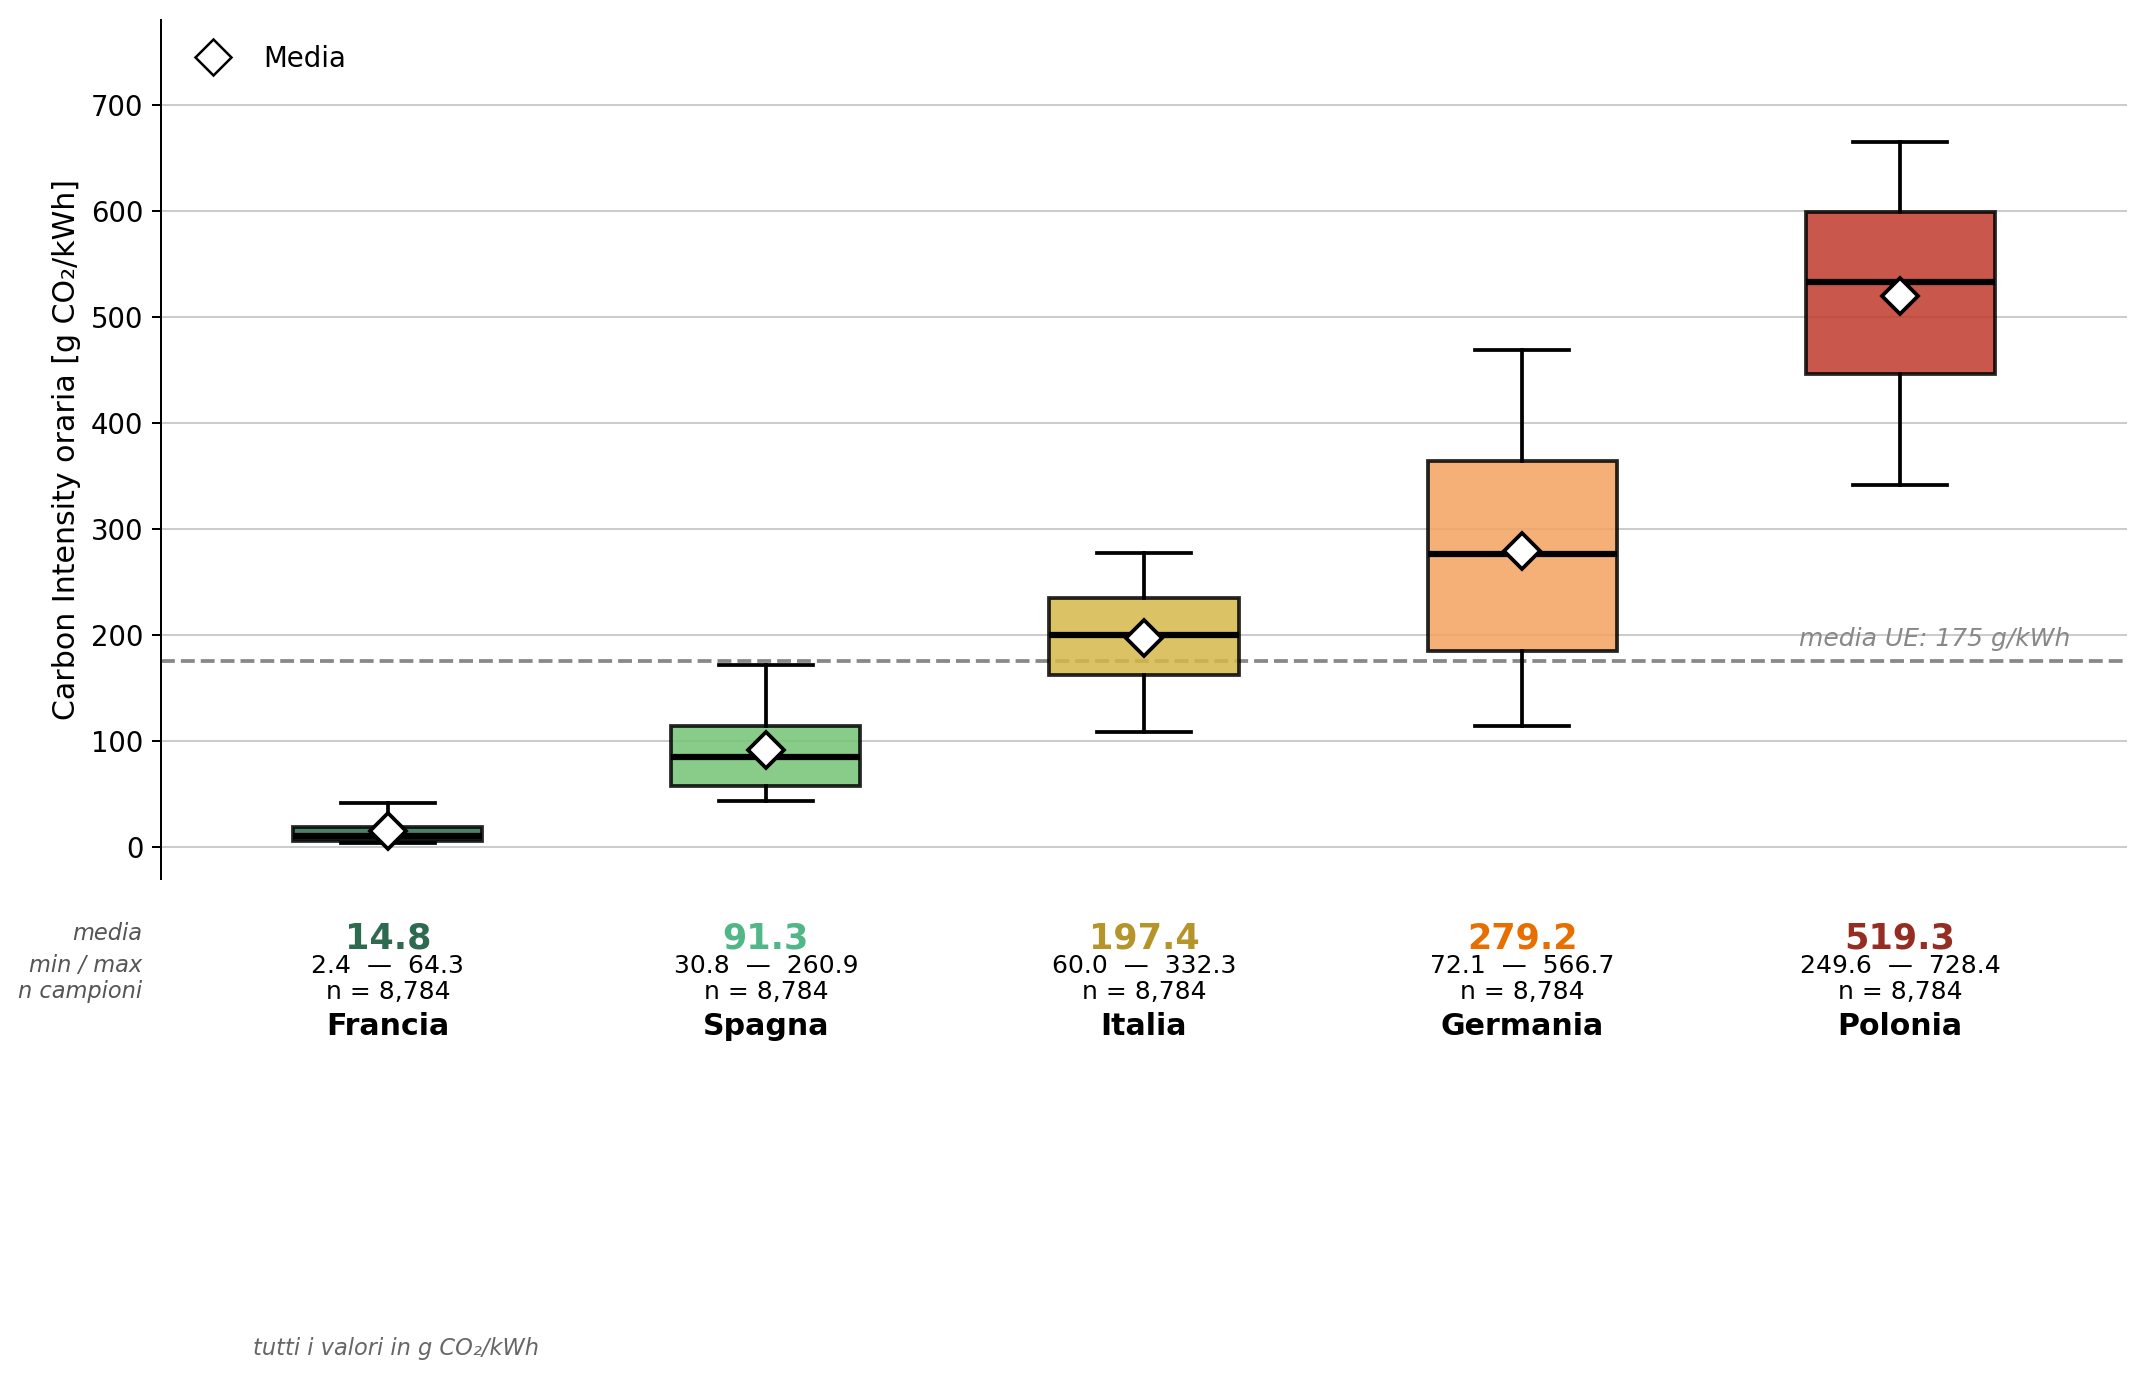
\includegraphics[width=0.95\textwidth]{figures/boxplot_ci_full (1).png}
    \caption{Distribuzione della carbon intensity oraria per zona nella
             traccia usata negli esperimenti. Le zone sono ordinate per
             CI media crescente da sinistra a destra.}
    \label{fig:ci-distribution-zone}
\end{figure}

% -----------------------------------------------------------
\section{Esperimento 1: calibrazione europea della carbon intensity}
\label{sec:esperimento1}
% -----------------------------------------------------------

\subsection{Obiettivo}
\label{subsec:esperimento1-obiettivo}

Il primo esperimento considera una politica carbon-aware in cui la funzione
sigmoide è fissata una sola volta a livello europeo. Le zone mantengono le
proprie tracce di carbon intensity, che possono avere valori e distribuzioni
molto diversi; ciò che resta invariato è la funzione che converte ciascun
valore di CI nel parametro $\lambda$. L'esperimento serve quindi a osservare
come cambiano le scelte dello scheduler quando segnali carbonici diversi
vengono interpretati tramite la stessa mappa decisionale.

\subsection{Configurazione}
\label{subsec:esperimento1-configurazione}

La normalizzazione del segnale di carbon intensity utilizza una sigmoide
calibrata su un riferimento europeo comune, con punto medio fissato al
valore medio europeo. In questo modo la medesima funzione
$\lambda(\mathrm{CI})$ viene applicata a tutte le zone, pur in presenza di
tracce di CI differenti. Le differenze osservate dipendono quindi dai
valori di CI propri di ciascuna zona e dalla loro posizione rispetto alla
sigmoide comune. La Figura~\ref{fig:sigmoid-overlay} mostra la sigmoide
europea e la collocazione delle zone lungo l'asse decisionale.

\begin{figure}[H]
    \centering
    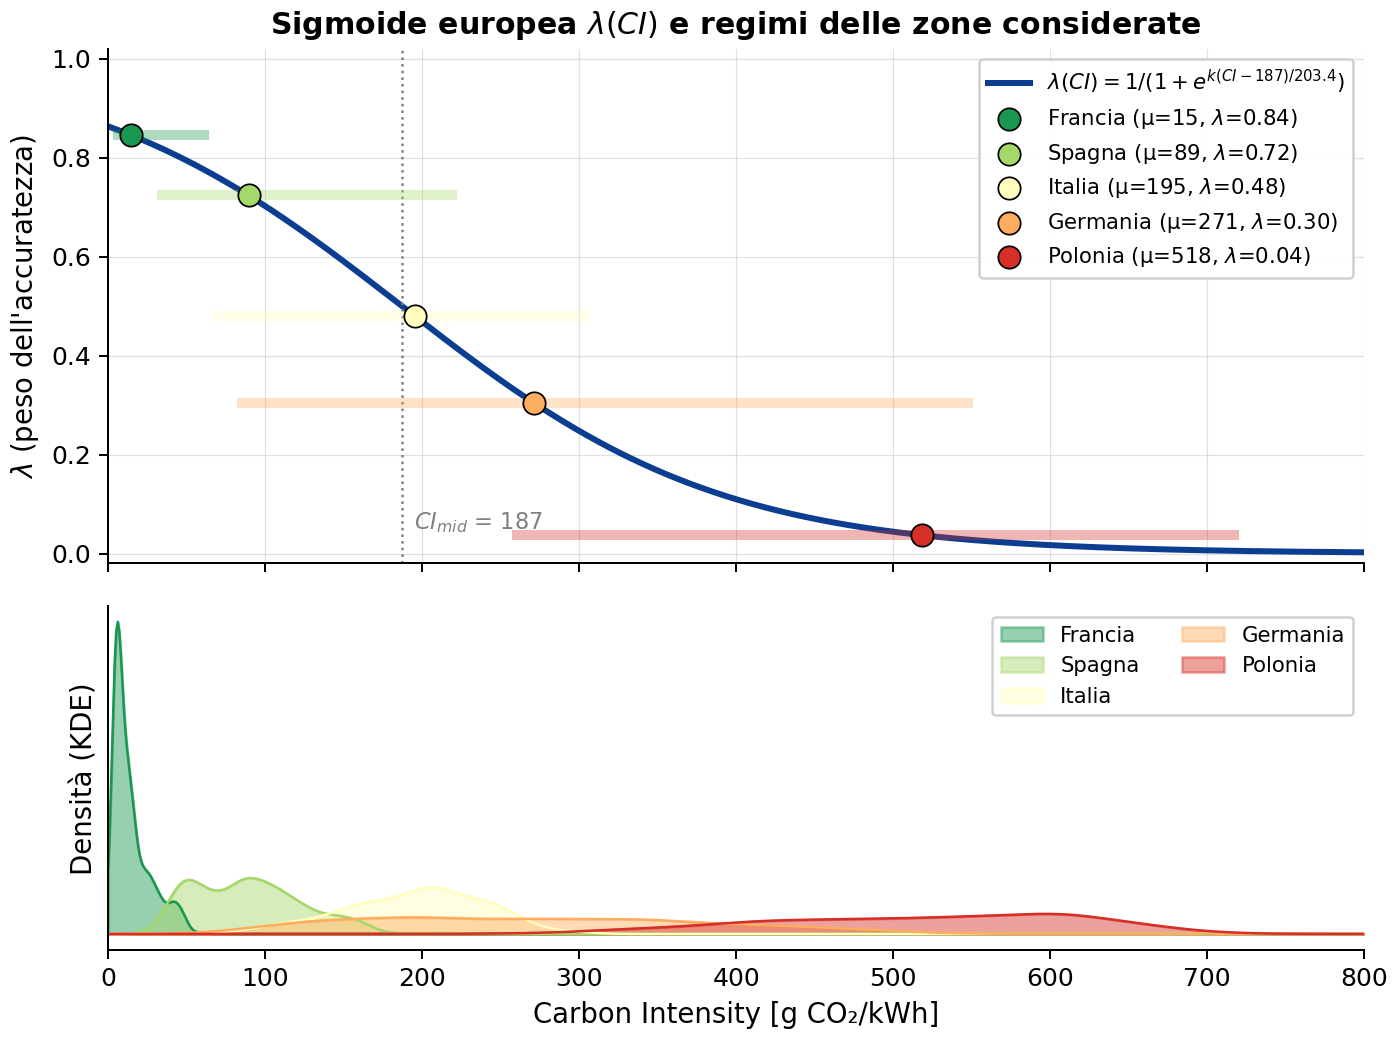
\includegraphics[width=0.95\textwidth]{figures/validation/06_sigmoid_overlay.png}
    \caption{Sigmoide europea utilizzata per trasformare la CI nel
             parametro $\lambda$ e collocazione delle zone considerate.
             La funzione mappa le CI più basse verso $\lambda \approx 1$
             (preferenza per la qualità) e le CI più alte verso
             $\lambda \approx 0$ (preferenza per il risparmio energetico).}
    \label{fig:sigmoid-overlay}
\end{figure}

Per ogni coppia funzione-zona viene eseguita la stessa traccia nei tre
regimi \emph{always-accurate}, \emph{always-energy} e carbon-aware:
864 invocazioni per coppia nelle funzioni numeriche e 576 nelle funzioni ML.

\paragraph{Metriche raccolte.}
Per ogni invocazione vengono raccolte tre metriche: l'energia consumata,
espressa come valore totale e come media per invocazione; il tempo medio
di esecuzione per invocazione, espresso in millisecondi; e la distribuzione
percentuale delle varianti selezionate dallo scheduler nelle cinque zone.

\subsection{Risultati}
\label{subsec:esperimento1-risultati}

Un primo indicatore del comportamento dello scheduler è la distribuzione
delle varianti selezionate. Le Figure~\ref{fig:variant-distribution-numeric-exp1}
e~\ref{fig:variant-distribution-ml-exp1} riportano, per ciascuna funzione,
la composizione percentuale delle varianti scelte dallo scheduler con
calibrazione europea nelle cinque zone, ordinate per CI media crescente.

\begin{figure}[p]
    \centering
    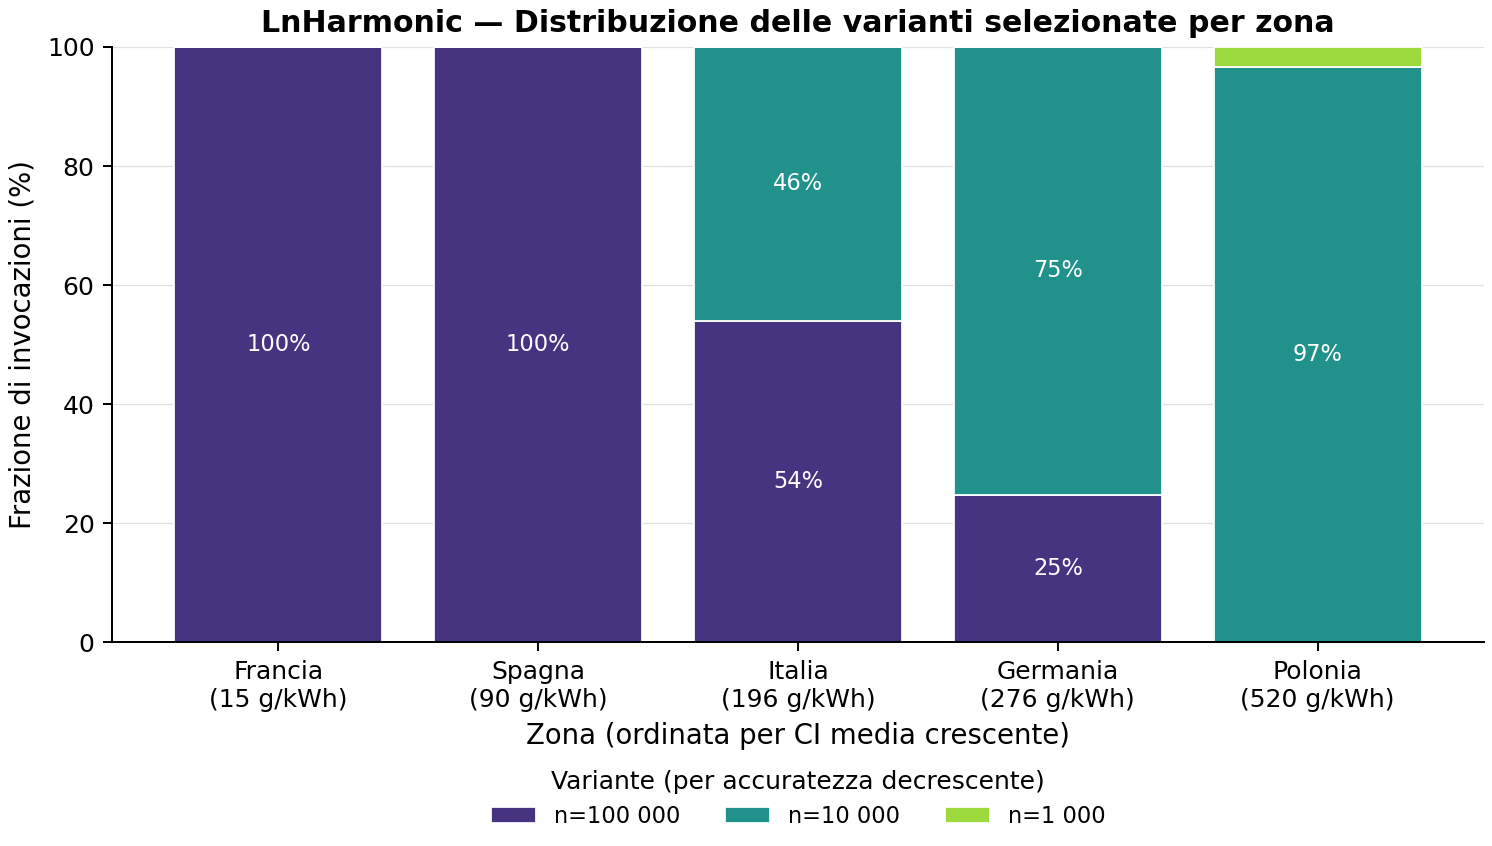
\includegraphics[width=0.72\textwidth]{figures/validation/01_variant_distribution_LnHarmonic.png}
    \vspace{0.2cm}
    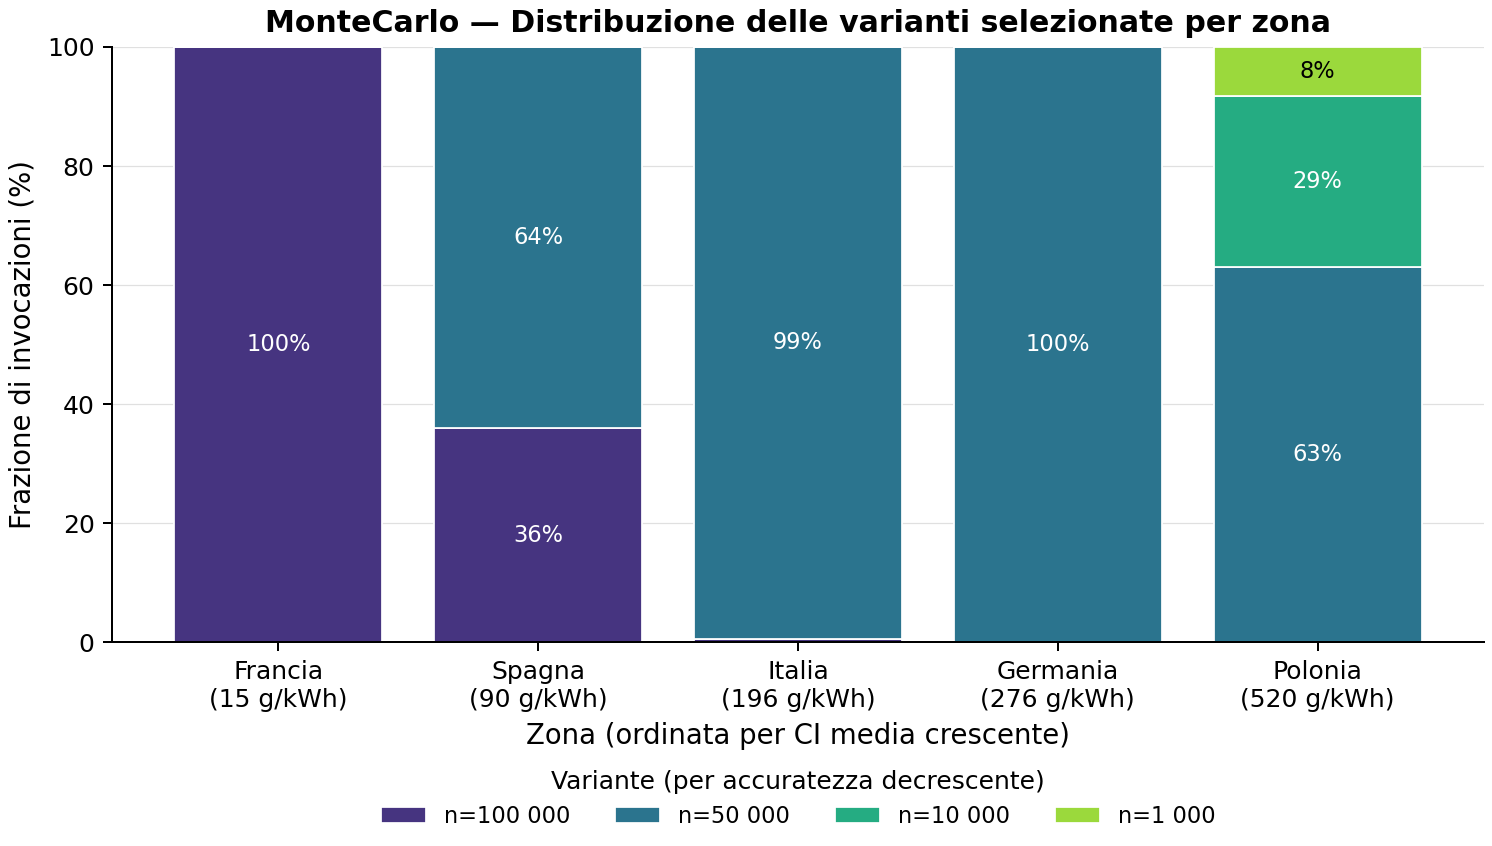
\includegraphics[width=0.72\textwidth]{figures/validation/01_variant_distribution_MonteCarlo.png}
    \vspace{0.2cm}
    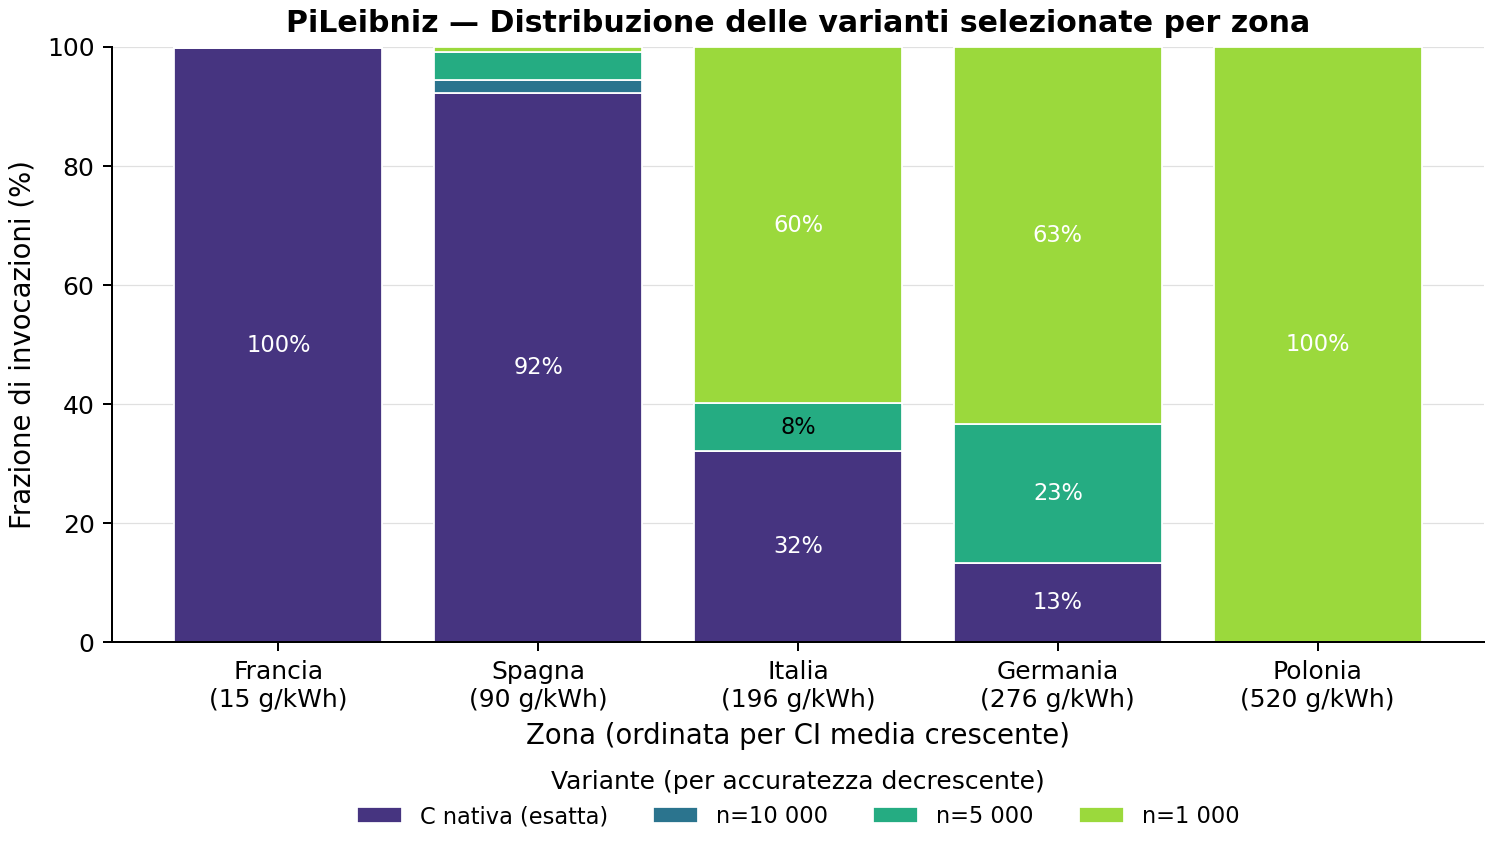
\includegraphics[width=0.72\textwidth]{figures/validation/01_variant_distribution_PiLeibniz.png}
    \caption{Distribuzione delle varianti selezionate per le funzioni
             numeriche nell'Esperimento~1. Al crescere della CI media, la
             quota delle varianti più accurate si riduce a favore di
             varianti a minore consumo, con una granularità che dipende
             dalla frontiera di Pareto della singola funzione.}
    \label{fig:variant-distribution-numeric-exp1}
\end{figure}

\begin{figure}[p]
    \centering
    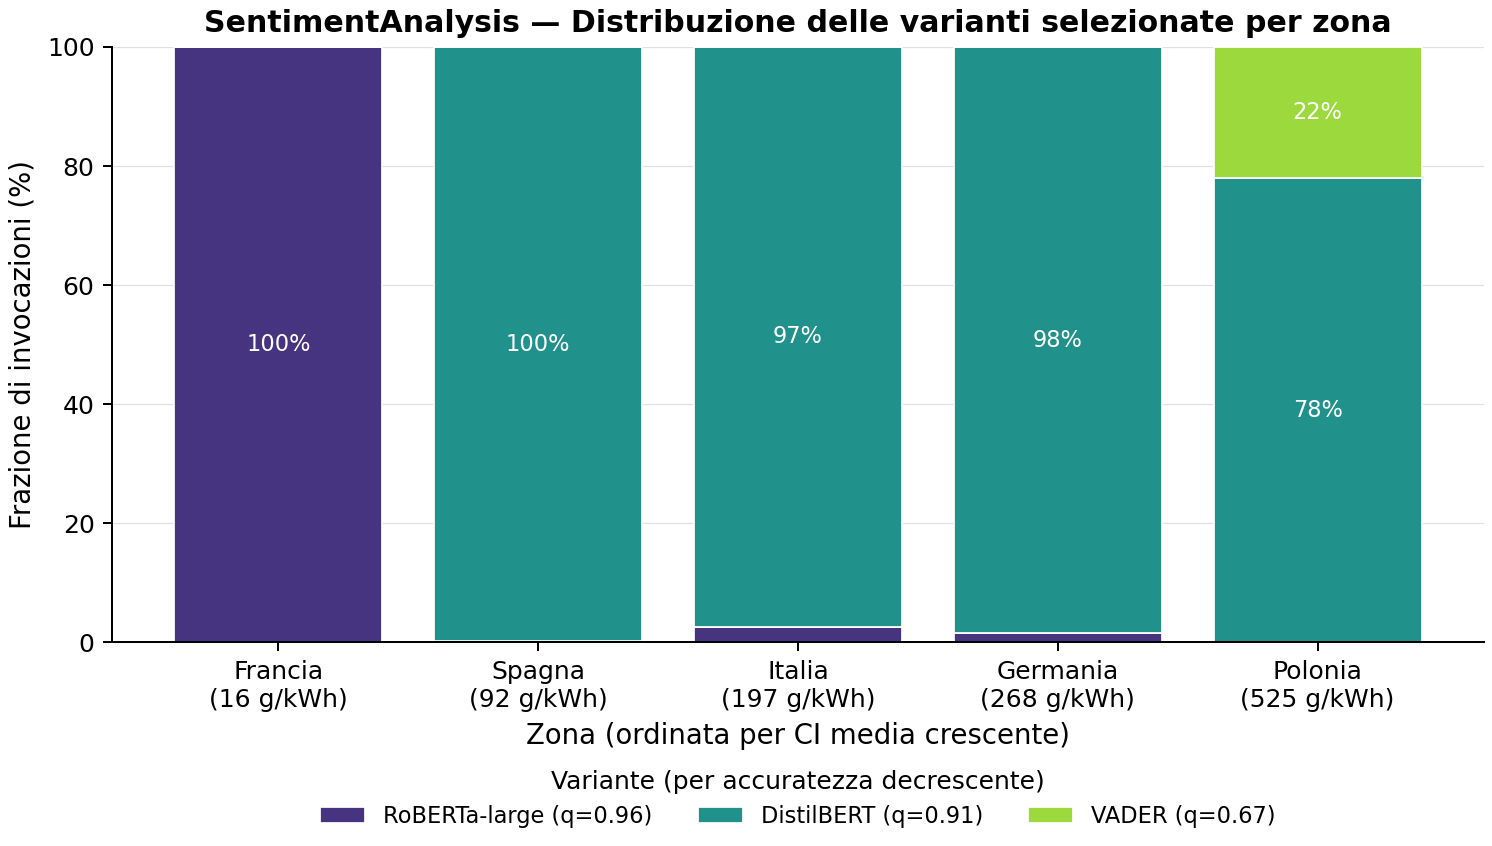
\includegraphics[width=0.72\textwidth]{figures/validation/01_variant_distribution_SentimentAnalysis.png}
    \vspace{0.2cm}
    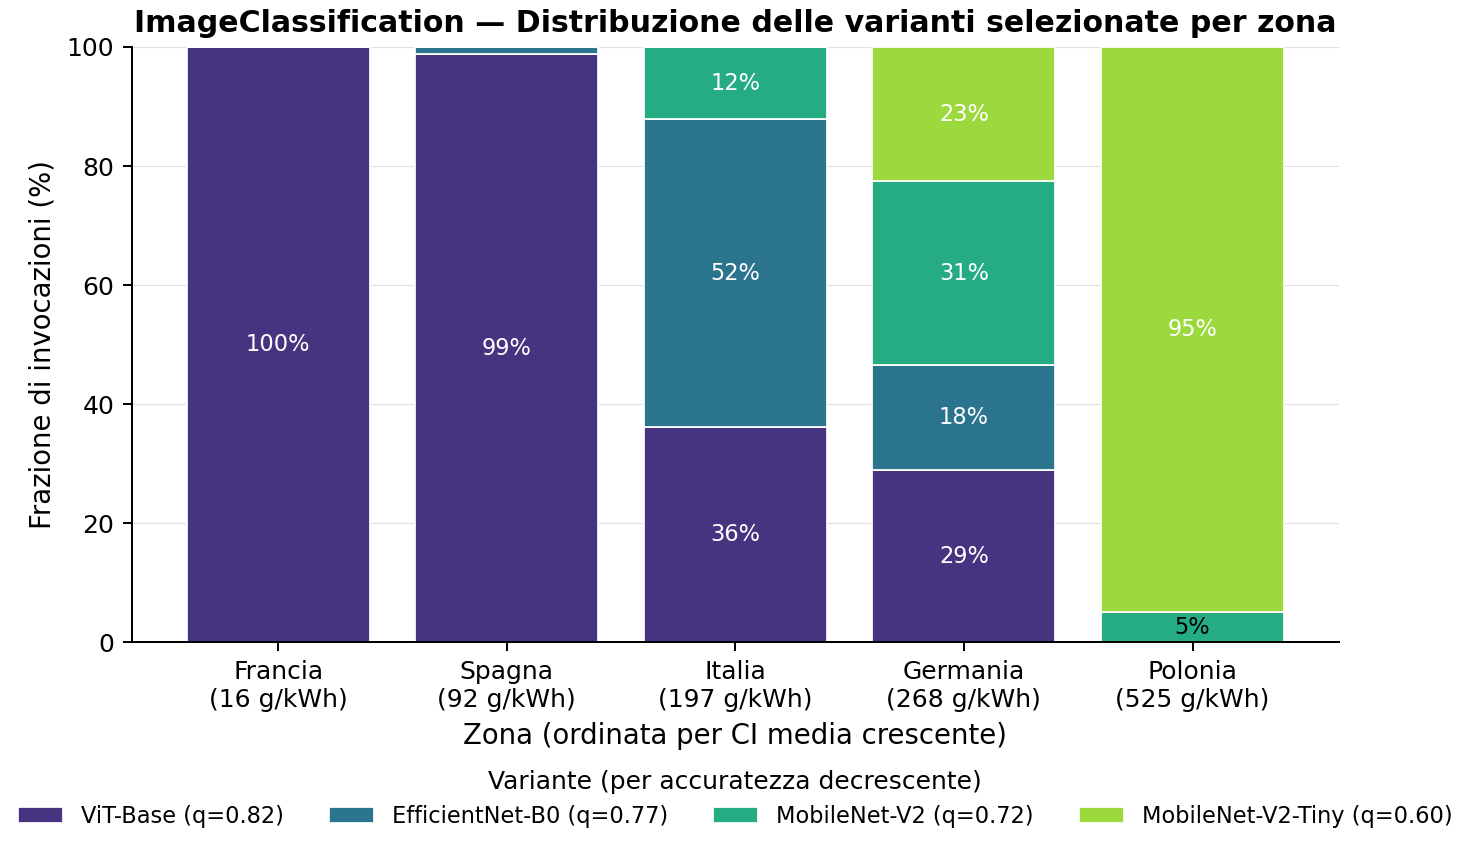
\includegraphics[width=0.72\textwidth]{figures/validation/01_variant_distribution_ImageClassification.png}
    \vspace{0.2cm}
    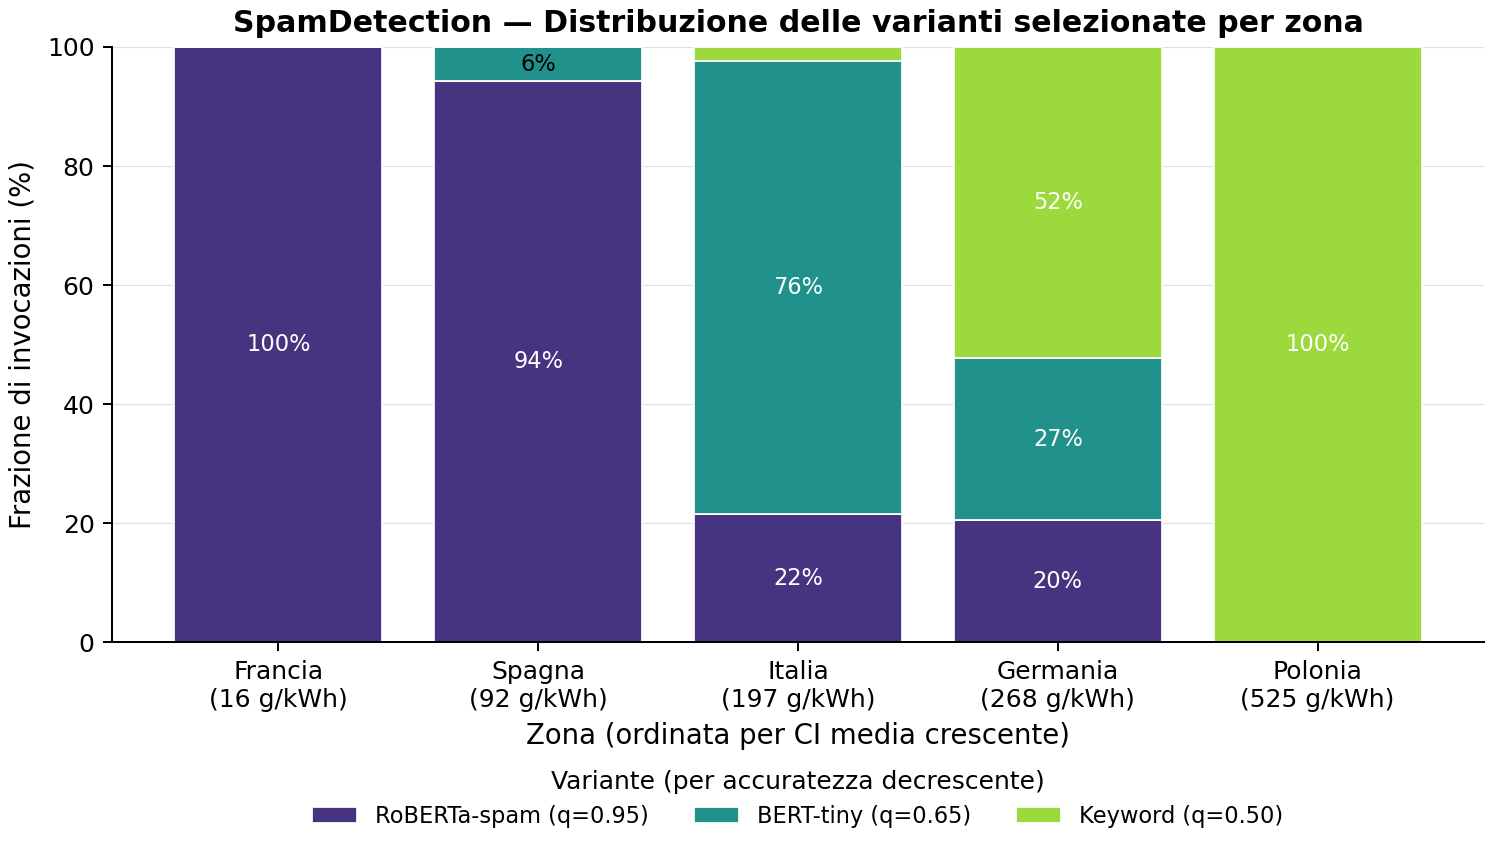
\includegraphics[width=0.72\textwidth]{figures/validation/01_variant_distribution_SpamDetection.png}
    \caption{Distribuzione delle varianti selezionate per le funzioni ML
             nell'Esperimento~1. Le transizioni tra varianti sono più
             discrete rispetto alle funzioni numeriche, poiché ciascuna
             variante corrisponde a un modello architetturalmente distinto.}
    \label{fig:variant-distribution-ml-exp1}
\end{figure}

\paragraph{Funzioni numeriche.}
Per le funzioni numeriche il comportamento è progressivo. In LnHarmonic,
Francia e Spagna selezionano la variante più accurata \texttt{n100000}
nel 100\% delle invocazioni; in Italia la stessa variante resta dominante
al 97\%, mentre in Germania la quota scende al 54\% e in Polonia al 25\%.
In parallelo cresce la quota di varianti meno costose: \texttt{n10000}
raggiunge il 46\% in Germania e il 75\% in Polonia, mentre \texttt{n1000}
compare solo in Polonia con il 3\%.

MonteCarlo mostra una transizione più netta: la Francia utilizza
\texttt{n100000} nel 100\% delle invocazioni, mentre Spagna e Italia
passano prevalentemente a \texttt{n50000}. In Polonia compaiono anche
\texttt{n10000} e \texttt{n1000}, con quote rispettivamente del 29\%
e dell'8\%. PiLeibniz presenta la frontiera più articolata: la variante
nativa in C domina in Francia, ma già in Spagna vengono selezionate anche
\texttt{n10000}, \texttt{n5000} e \texttt{n1000}. Questo comportamento è
coerente con la struttura della frontiera di Pareto della funzione,
illustrata in Figura~\ref{fig:pareto-setup}, e con le soglie di
selezione mostrate in Figura~\ref{fig:lambda-to-variant-setup}: diverse varianti
approssimate offrono scambi energia--errore non dominati e possono quindi
risultare ottimali per intervalli distinti di $\lambda$.

\paragraph{Funzioni ML.}
Per le funzioni ML le transizioni sono meno continue, poiché il numero di
modelli disponibili è ridotto e ogni modello corrisponde a un salto
architetturale discreto. In SentimentAnalysis la Francia seleziona
RoBERTa-large, mentre Spagna, Italia e Germania sono dominate da DistilBERT;
in Polonia compare VADER, variante più leggera e di conseguenza meno
accurata. ImageClassification è il caso in cui la variabilità decisionale
è più marcata: nella stessa zona (Germania) vengono selezionate ViT-Base,
EfficientNet-B0, MobileNet-V2 e MobileNet-V2-Tiny, a indicare che il
valore di $\lambda$ oscilla intorno a più soglie di transizione.
SpamDetection presenta invece una transizione più netta: RoBERTa-spam
è prevalente nelle zone a bassa CI, BERT-tiny nelle zone intermedie, e il
classificatore keyword diventa esclusivo in Polonia.

\paragraph{Trade-off aggregato.}
La Figura~\ref{fig:tradeoff-representative-exp1} riassume l'effetto
aggregato della selezione su due casi rappresentativi, uno numerico e uno
ML, mostrando energia media e qualità media al variare della zona.
L'energia media è calcolata come media pesata dei profili energetici delle
varianti selezionate, quindi dipende dalla distribuzione delle scelte
orarie e non solo dalla CI media della zona. In PiLeibniz l'energia scende
da 1.05~mJ in Francia a 0.20~mJ in Polonia, mantenendo una perdita
qualitativa contenuta. In SpamDetection il risparmio è più marcato, ma la
transizione verso il classificatore keyword porta a una riduzione
qualitativa evidente: questo caso mostra che il costo del risparmio
energetico non è uniforme e dipende dalla struttura della frontiera di
Pareto della specifica funzione.

\begin{figure}[p]
    \centering
    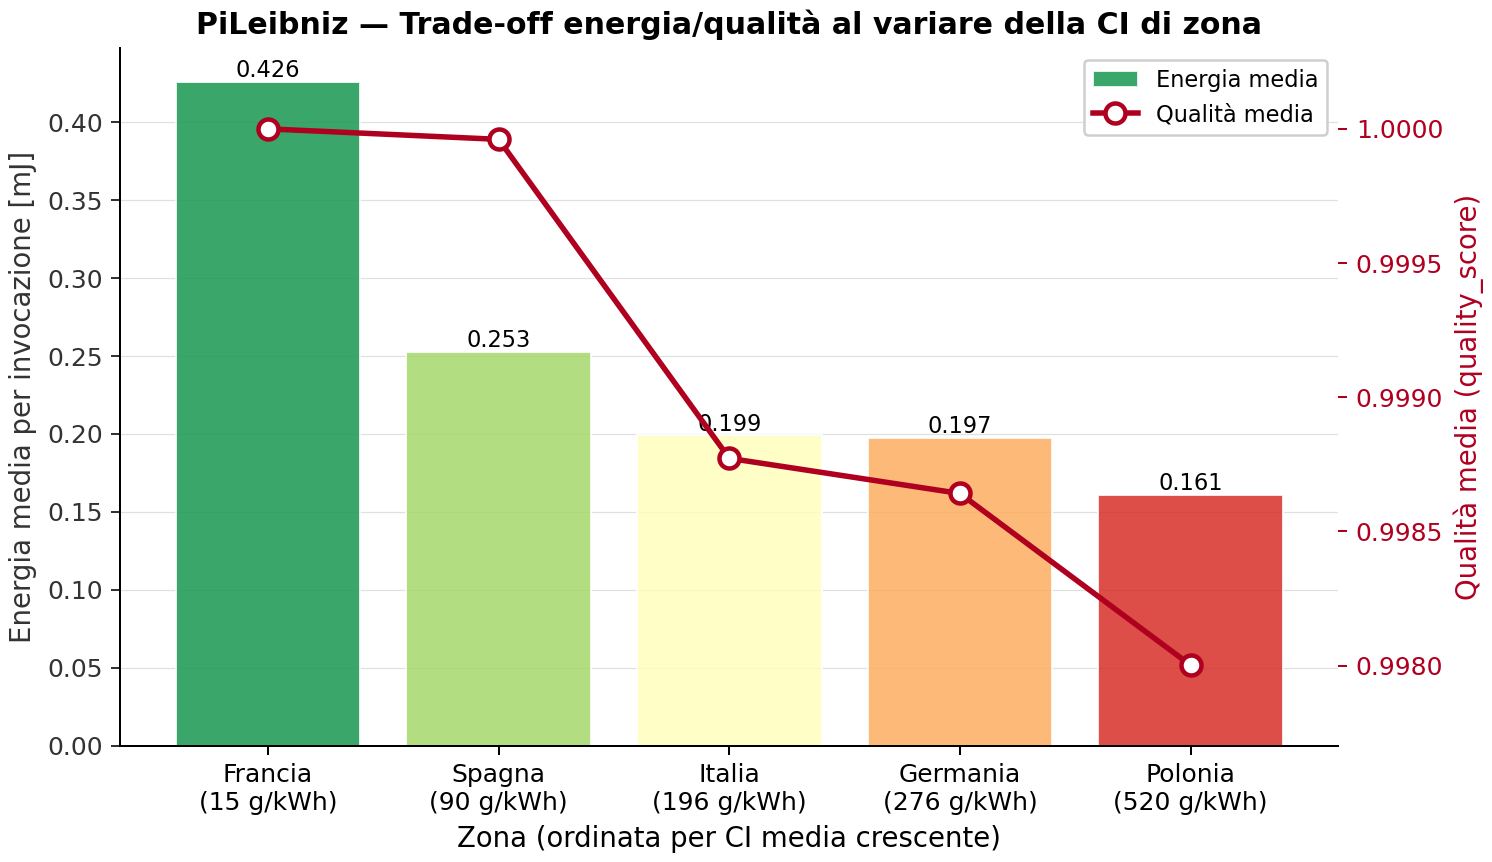
\includegraphics[width=0.78\textwidth]{figures/validation/03_tradeoff_PiLeibniz.png}
    \vspace{0.2cm}
    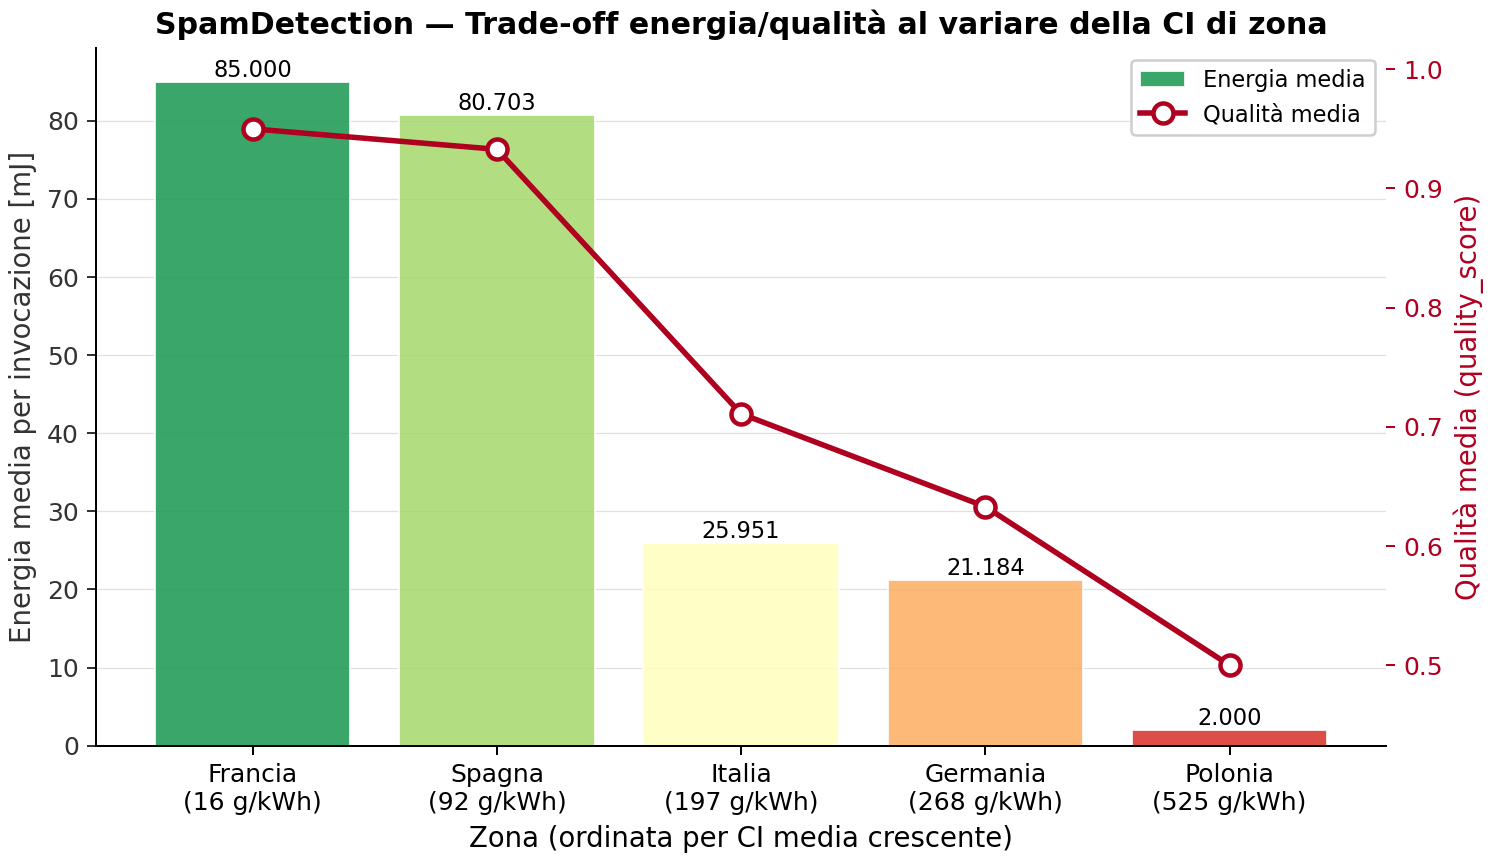
\includegraphics[width=0.78\textwidth]{figures/validation/03_tradeoff_SpamDetection.png}
    \caption{Trade-off energia--qualità per due funzioni rappresentative
             nell'Esperimento~1. PiLeibniz mostra una riduzione progressiva
             dell'energia con perdita qualitativa contenuta; SpamDetection
             evidenzia invece un risparmio più netto accompagnato da un costo
             qualitativo maggiore quando viene selezionata la variante
             keyword.}
    \label{fig:tradeoff-representative-exp1}
\end{figure}

Il confronto con le baseline quantifica la posizione dello scheduler tra
due estremi: \emph{always-accurate}, che privilegia sempre la qualità, e
\emph{always-energy}, che privilegia sempre il consumo minimo. La
Tabella~\ref{tab:baseline-comparison-exp1} riporta, per energia, qualità e tempi di risposta,
la variazione percentuale dello scheduler rispetto a entrambe le baseline.
Un valore negativo di $\Delta E$ e $\Delta T$ indica che lo scheduler consuma meno della baseline, mentre un
valore positivo di $\Delta Q$ indica che ottiene una qualità media superiore.



% ─────────────────────────────────────────────────────────────────────────────
% Tabella: variazione % dello scheduler carbon-aware rispetto alle due baseline.
% Energia: solo invocation_joule (cold start MAI incluso).
% Qualità: quality_score (funzioni ML) oppure 1 − error_estimate (funzioni numeriche).
% ΔE_acc, ΔQ_acc : scarto vs always-accurate (Λ₁, massima qualità Pareto)
% ΔE_ene, ΔQ_ene : scarto vs always-energy  (Λ₀, minima energia Pareto)
% Valori negativi di ΔE → risparmio energetico rispetto alla baseline.
% Valori positivi  di ΔQ → qualità superiore alla baseline.
% ─────────────────────────────────────────────────────────────────────────────

\begin{table}[H]
    \centering
    \caption{Variazione percentuale dello scheduler carbon-aware rispetto
             alle due baseline. $\Delta E_{acc}$, $\Delta T_{acc}$,
             $\Delta Q_{acc}$: scarto rispetto ad \emph{always-accurate}
             ($\Lambda_1$); $\Delta E_{ene}$, $\Delta T_{ene}$,
             $\Delta Q_{ene}$: scarto rispetto ad \emph{always-energy}
             ($\Lambda_0$). Valori negativi di $\Delta E$ e $\Delta T$
             indicano un risparmio rispetto alla baseline; valori positivi
             di $\Delta Q$ indicano qualità superiore alla baseline.}
    \label{tab:baseline-comparison-exp1}
    \resizebox{\textwidth}{!}{%
    \begin{tabular}{llrrrrrr}
        \toprule
        Funzione & Zona
            & $\Delta E_{acc}$ & $\Delta T_{acc}$ & $\Delta Q_{acc}$
            & $\Delta E_{ene}$ & $\Delta T_{ene}$ & $\Delta Q_{ene}$ \\
        \midrule
        % ── PiLeibniz ──────────────────────────────────────────────────────────
        % Λ₁ = C-nativa  (E=0.001052 J, error=0.0)
        % Λ₀ = n=1 000   (E=0.000196 J, error=0.001999)
        PiLeibniz   & Francia
            & $0.00$\%  & $0.00$\%  & $0.00$\%
            & \redval{$+436.73$\%}  & \redval{$+318.40$\%}  & \greenval{$+0.20$\%} \\
                    & Spagna
            & \greenval{$-5.34$\%}  & \greenval{$-3.92$\%}  & \redval{$-0.00$\%}
            & \redval{$+408.10$\%}  & \redval{$+298.60$\%}  & \greenval{$+0.20$\%} \\
                    & Italia
            & \greenval{$-53.62$\%} & \greenval{$-39.14$\%} & \redval{$-0.12$\%}
            & \redval{$+148.94$\%}  & \redval{$+109.22$\%}  & \greenval{$+0.08$\%} \\
                    & Germania
            & \greenval{$-68.34$\%} & \greenval{$-50.87$\%} & \redval{$-0.14$\%}
            & \redval{$+69.92$\%}   & \redval{$+51.38$\%}   & \greenval{$+0.06$\%} \\
                    & Polonia
            & \greenval{$-81.37$\%} & \greenval{$-60.53$\%} & \redval{$-0.20$\%}
            & $0.00$\%  & $0.00$\%  & $0.00$\% \\
        \midrule
        % ── LnHarmonic ─────────────────────────────────────────────────────────
        % Λ₁ = base       (E=0.007700 J, error=0.0)
        % Λ₀ = n=1 000    (E=0.000196 J, error=0.001440)
        LnHarmonic  & Francia
            & $0.00$\%  & $0.00$\%  & $0.00$\%
            & \redval{$+493.37$\%}  & \redval{$+376.40$\%}  & \greenval{$+0.14$\%} \\
                    & Spagna
            & $0.00$\%  & $0.00$\%  & $0.00$\%
            & \redval{$+493.37$\%}  & \redval{$+376.40$\%}  & \greenval{$+0.14$\%} \\
                    & Italia
            & \greenval{$-89.33$\%} & \greenval{$-70.82$\%} & \redval{$-0.01$\%}
            & \redval{$+319.22$\%}  & \redval{$+241.60$\%}  & \greenval{$+0.14$\%} \\
                    & Germania
            & \greenval{$-92.12$\%} & \greenval{$-74.36$\%} & \redval{$-0.01$\%}
            & \redval{$+209.44$\%}  & \redval{$+159.30$\%}  & \greenval{$+0.13$\%} \\
                    & Polonia
            & \greenval{$-94.62$\%} & \greenval{$-77.19$\%} & \redval{$-0.02$\%}
            & \redval{$+111.35$\%}  & \redval{$+84.70$\%}   & \greenval{$+0.13$\%} \\
        \midrule
        % ── MonteCarlo ─────────────────────────────────────────────────────────
        % Λ₁ = n=500 000  (E=0.231480 J, error=0.00232)
        % Λ₀ = n=1 000    (E=0.000147 J, error=0.052)
        MonteCarlo  & Francia
            & \greenval{$-85.44$\%} & \greenval{$-68.35$\%} & \redval{$-0.29$\%}
            & \redval{$+22831.97$\%} & \redval{$+16924.30$\%} & \greenval{$+4.94$\%} \\
                    & Spagna
            & \greenval{$-90.80$\%} & \greenval{$-73.82$\%} & \redval{$-0.43$\%}
            & \redval{$+14384.80$\%} & \redval{$+10643.50$\%} & \greenval{$+4.79$\%} \\
                    & Italia
            & \greenval{$-93.82$\%} & \greenval{$-76.10$\%} & \redval{$-0.50$\%}
            & \redval{$+9633.26$\%}  & \redval{$+7091.80$\%}  & \greenval{$+4.71$\%} \\
                    & Germania
            & \greenval{$-93.82$\%} & \greenval{$-76.10$\%} & \redval{$-0.50$\%}
            & \redval{$+9633.26$\%}  & \redval{$+7091.80$\%}  & \greenval{$+4.71$\%} \\
                    & Polonia
            & \greenval{$-95.85$\%} & \greenval{$-78.23$\%} & \redval{$-1.13$\%}
            & \redval{$+6439.04$\%}  & \redval{$+4712.60$\%}  & \greenval{$+4.06$\%} \\
        \midrule
        % ── SentimentAnalysis ──────────────────────────────────────────────────
        % Λ₁ = RoBERTa-large (E=0.091579 J, q=0.964)
        % Λ₀ = VADER         (E=0.002400 J, q=0.674)
        SentimentAnalysis & Francia
            & $0.00$\%  & $0.00$\%  & $0.00$\%
            & \redval{$+3715.79$\%} & \redval{$+2812.50$\%} & \greenval{$+43.03$\%} \\
                    & Spagna
            & \greenval{$-57.74$\%} & \greenval{$-46.82$\%} & \redval{$-5.29$\%}
            & \redval{$+1512.50$\%} & \redval{$+1162.40$\%} & \greenval{$+35.46$\%} \\
                    & Italia
            & \greenval{$-56.01$\%} & \greenval{$-45.38$\%} & \redval{$-5.13$\%}
            & \redval{$+1578.60$\%} & \redval{$+1214.30$\%} & \greenval{$+35.69$\%} \\
                    & Germania
            & \greenval{$-56.59$\%} & \greenval{$-45.91$\%} & \redval{$-5.18$\%}
            & \redval{$+1556.57$\%} & \redval{$+1193.60$\%} & \greenval{$+35.61$\%} \\
                    & Polonia
            & \greenval{$-66.46$\%} & \greenval{$-54.12$\%} & \redval{$-10.74$\%}
            & \redval{$+1179.75$\%} & \redval{$+892.30$\%}  & \greenval{$+27.66$\%} \\
        \midrule
        % ── SpamDetection ──────────────────────────────────────────────────────
        % Λ₁ = RoBERTa-spam (E=0.085000 J, q=0.995)
        % Λ₀ = Keyword      (E=0.002000 J, q=0.720)
        SpamDetection & Francia
            & $0.00$\%  & $0.00$\%  & $0.00$\%
            & \redval{$+4150.00$\%} & \redval{$+3087.50$\%} & \greenval{$+38.19$\%} \\
                    & Spagna
            & \greenval{$-5.29$\%}  & \greenval{$-3.97$\%}  & \redval{$-0.27$\%}
            & \redval{$+3925.00$\%} & \redval{$+2916.40$\%} & \greenval{$+37.82$\%} \\
                    & Italia
            & \greenval{$-69.01$\%} & \greenval{$-52.48$\%} & \redval{$-3.99$\%}
            & \redval{$+1217.00$\%} & \redval{$+905.60$\%}  & \greenval{$+32.68$\%} \\
                    & Germania
            & \greenval{$-75.58$\%} & \greenval{$-57.14$\%} & \redval{$-15.87$\%}
            & \redval{$+938.00$\%}  & \redval{$+698.80$\%}  & \greenval{$+16.26$\%} \\
                    & Polonia
            & \greenval{$-97.65$\%} & \greenval{$-74.38$\%} & \redval{$-27.64$\%}
            & $0.00$\%  & $0.00$\%  & $0.00$\% \\
        \midrule
        % ── ImageClassification ────────────────────────────────────────────────
        % Λ₁ = ViT-Base          (E=1.455263 J, q=0.818)
        % Λ₀ = MobileNet-V2-Tiny (E=0.077000 J, q=0.603)
        ImageClassification & Francia
            & $0.00$\%  & $0.00$\%  & $0.00$\%
            & \redval{$+1789.95$\%} & \redval{$+1347.20$\%} & \greenval{$+35.66$\%} \\
                    & Spagna
            & \greenval{$-0.71$\%}  & \greenval{$-0.58$\%}  & \redval{$-0.06$\%}
            & \redval{$+1776.48$\%} & \redval{$+1334.80$\%} & \greenval{$+35.58$\%} \\
                    & Italia
            & \greenval{$-47.18$\%} & \greenval{$-38.12$\%} & \redval{$-4.45$\%}
            & \redval{$+898.35$\%}  & \redval{$+678.40$\%}  & \greenval{$+29.61$\%} \\
                    & Germania
            & \greenval{$-60.13$\%} & \greenval{$-48.67$\%} & \redval{$-10.76$\%}
            & \redval{$+653.44$\%}  & \redval{$+492.30$\%}  & \greenval{$+21.06$\%} \\
                    & Polonia
            & \greenval{$-93.54$\%} & \greenval{$-75.42$\%} & \redval{$-25.26$\%}
            & \redval{$+22.14$\%}   & \redval{$+16.82$\%}   & \greenval{$+1.39$\%} \\
        \bottomrule
    \end{tabular}
    }
\end{table}

\subsection{Interpretazione}
\label{subsec:esperimento1-interpretazione}

I risultati mostrano l'effetto della calibrazione europea sulle scelte
dello scheduler. Poiché tutte le zone sono valutate rispetto alla stessa
funzione $\lambda(\mathrm{CI})$, le reti con CI mediamente più bassa, come
la Francia, ricadono più spesso in regioni che privilegiano la qualità,
mentre le reti con CI più elevata, come la Polonia, ricadono più spesso in
regioni che favoriscono il risparmio energetico.

La Tabella~\ref{tab:baseline-comparison-exp1} rende visibile questo
spostamento. Nelle zone a bassa CI lo scheduler tende a coincidere con
\emph{always-accurate}: in Francia, ad esempio, diverse funzioni non
mostrano alcuna perdita di qualità rispetto alla baseline più accurata.
Al crescere della CI, invece, aumentano gli scostamenti negativi in energia
e tempo rispetto ad \emph{always-accurate}. Questo indica che la politica
inizia a selezionare varianti più leggere, accettando una degradazione
controllata della qualità. Il fenomeno è particolarmente evidente in
Polonia, dove le riduzioni energetiche rispetto alla baseline accurata
diventano molto marcate, soprattutto per le funzioni con un ampio divario
tra variante più accurata e variante più efficiente.

Il confronto con \emph{always-energy} mostra il lato opposto del
compromesso. Lo scheduler, nella maggior parte dei casi, consuma più della
baseline energeticamente minima, ma mantiene una qualità media superiore.
Questo comportamento è atteso: la politica carbon-aware non cerca
semplicemente di minimizzare il consumo locale, ma di scegliere un punto
intermedio sulla frontiera energia--qualità in funzione della CI osservata.
Quando la rete è molto carbon-intensive, tale punto si avvicina alla
baseline energetica; quando la rete è poco carbon-intensive, si avvicina
alla baseline accurata.



% -----------------------------------------------------------
\section{Esperimento 2: calibrazione locale della carbon intensity}
\label{sec:esperimento2}
% -----------------------------------------------------------

\subsection{Obiettivo}
\label{subsec:esperimento2-obiettivo}

Il secondo esperimento valuta lo stesso scheduler in una configurazione
locale. A differenza dell'Esperimento~1, in cui tutte le zone condividono
un riferimento europeo, qui la sigmoide è calibrata sulla distribuzione
storica di ciascuna zona. Il valore di $\lambda$ non dipende quindi
soltanto dalla CI assoluta, ma anche dalla sua posizione rispetto al regime
abituale della rete considerata. Questa configurazione rappresenta il caso
più vicino a un deployment reale, in cui un nodo interpreta il segnale
carbon-aware rispetto al contesto elettrico in cui opera.

\subsection{Configurazione}
\label{subsec:esperimento2-configurazione}

La struttura sperimentale è la stessa dell'Esperimento~1: per ogni zona
viene rieseguita la stessa traccia nei tre regimi. Cambia la
normalizzazione del segnale ambientale: per ogni zona $z$, la sigmoide
utilizza la media storica locale $\mu_z$ e i percentili locali $P_5$ e
$P_{95}$ stimati dalle serie ElectricityMaps~\cite{electricitymaps2024};
la Figura~\ref{fig:exp2-sigmoidi-locali} mostra due esempi rappresentativi
di questa calibrazione.
La stessa CI assoluta può generare valori di $\lambda$ differenti in zone
diverse, poiché rappresenta una condizione ordinaria in una rete e
un'anomalia in un'altra: questo aspetto motiva l'adozione di una
calibrazione locale rispetto a una soglia globale uniforme.

Nell'Esperimento~2 la traccia di carbon intensity non viene campionata per
giornate prestabilite, come nell'Esperimento~1, ma a livello di singoli
timestamp orari. A partire dalla distribuzione annuale della CI di ciascuna
zona, i valori orari sono ordinati e suddivisi in tre fasce
rappresentative: bassa, media e alta intensità carbonica. Da ciascuna fascia
viene selezionato lo stesso numero di timestamp, ottenendo un campione
complessivo di 120 punti per zona.

Questo permette di osservare lo scheduler in condizioni ambientali
eterogenee e rilevanti per la decisione carbon-aware. Rispetto a un
campionamento basato su giornate intere fissate a priori, il campionamento
per timestamp distribuisce meglio le misure lungo l'intervallo di valori
della CI, includendo sia condizioni in cui la rete è relativamente pulita
sia condizioni più carbon-intensive. In questo modo il confronto tra
\emph{always-energy}, carbon-aware e \emph{always-accurate} viene effettuato
su punti che coprono in modo più diretto le diverse regioni della funzione
$\lambda(\mathrm{CI})$. La Figura~\ref{fig:exp2-ci-distribution-sampling}
mostra, per ciascuna zona, la distribuzione annuale della CI e la
suddivisione usata per individuare le fasce di campionamento.

\begin{figure}[p]
    \centering
    \begin{subfigure}{0.49\textwidth}
        \centering
        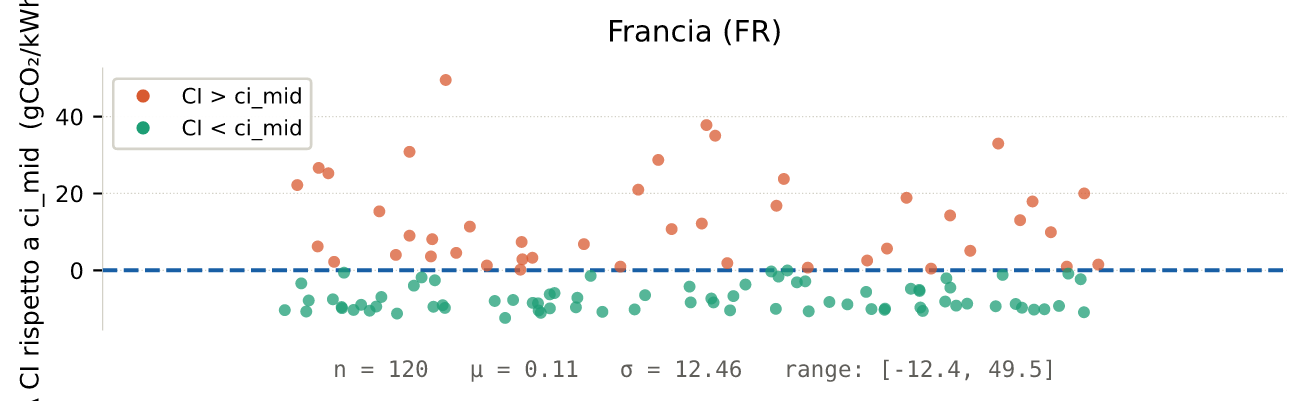
\includegraphics[width=\textwidth]{figures/ci_distribution_FR.png}
        \caption{Francia (FR)}
    \end{subfigure}
    \hfill
    \begin{subfigure}{0.49\textwidth}
        \centering
        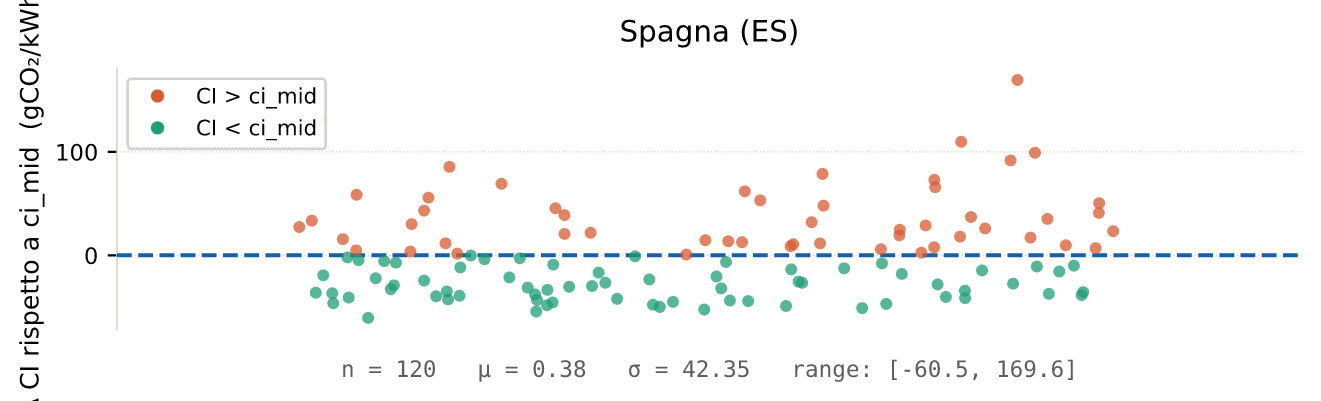
\includegraphics[width=\textwidth]{figures/ci_distribution_ES.png}
        \caption{Spagna (ES)}
    \end{subfigure}

    \vspace{0.25cm}
    \begin{subfigure}{0.49\textwidth}
        \centering
        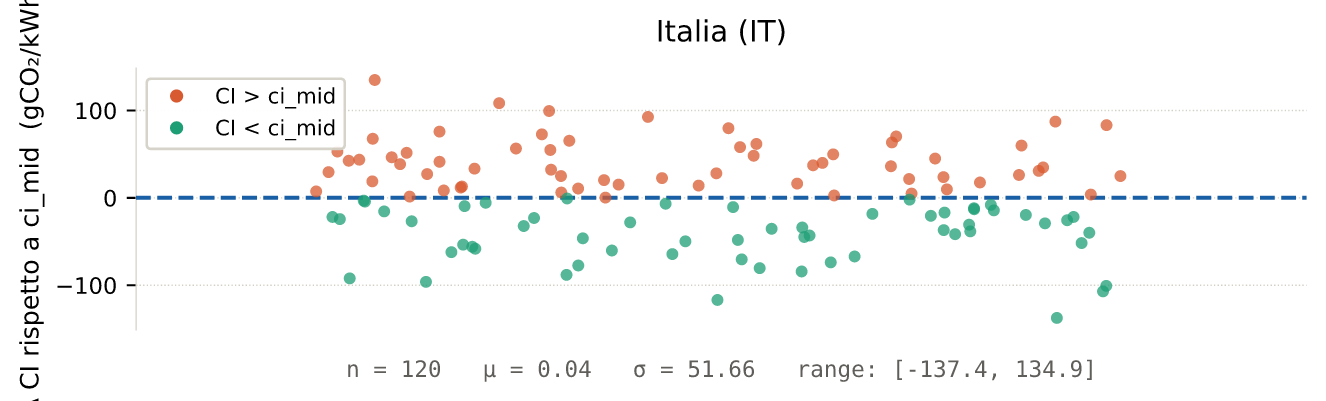
\includegraphics[width=\textwidth]{figures/ci_distribution_IT.png}
        \caption{Italia (IT)}
    \end{subfigure}
    \hfill
    \begin{subfigure}{0.49\textwidth}
        \centering
        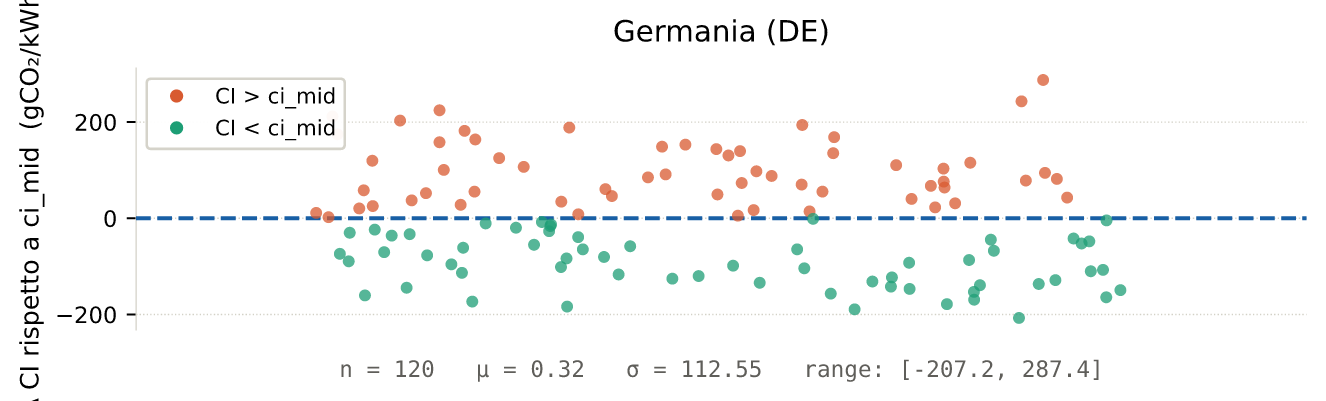
\includegraphics[width=\textwidth]{figures/ci_distribution_DE.png}
        \caption{Germania (DE)}
    \end{subfigure}

    \vspace{0.25cm}
    \begin{subfigure}{0.49\textwidth}
        \centering
        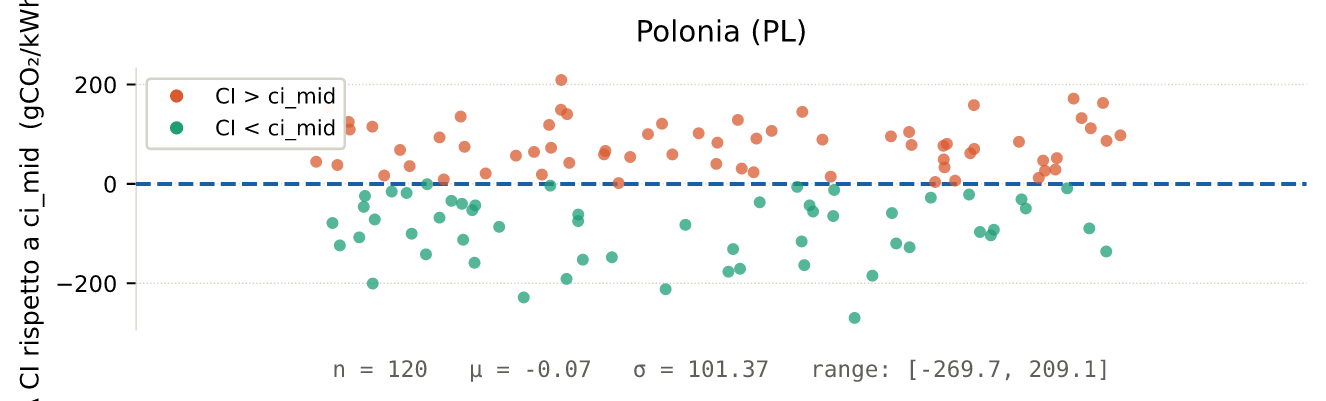
\includegraphics[width=\textwidth]{figures/ci_distribution_PL.png}
        \caption{Polonia (PL)}
    \end{subfigure}
    \caption{Distribuzione annuale della carbon intensity per zona e fasce
             utilizzate per il campionamento dei timestamp dell'Esperimento~2.
             La selezione bilanciata tra valori bassi, medi e alti evita che
             il campione sia concentrato solo attorno alle condizioni più
             frequenti della rete.}
    \label{fig:exp2-ci-distribution-sampling}
\end{figure}

\begin{figure}[p]
    \centering
    \begin{subfigure}{0.80\textwidth}
        \centering
        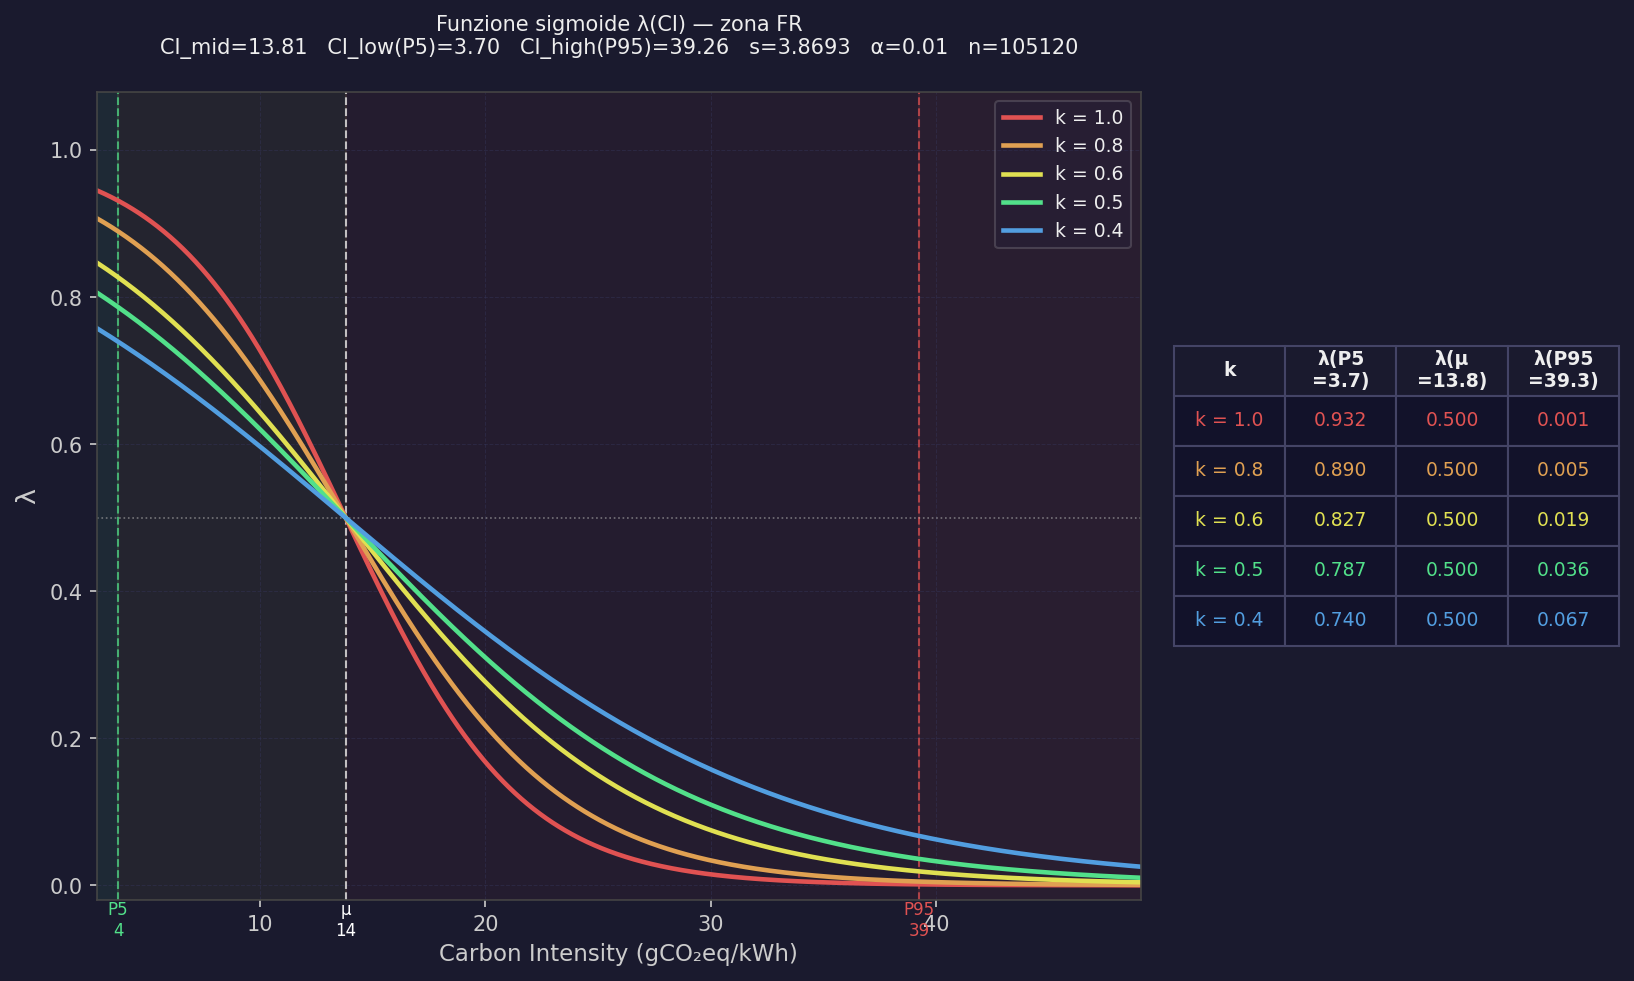
\includegraphics[width=\textwidth]{figures/lambda_curve_FR.png}
        \caption{Francia (FR)}
    \end{subfigure}

    \vspace{0.25cm}
    \begin{subfigure}{0.80\textwidth}
        \centering
        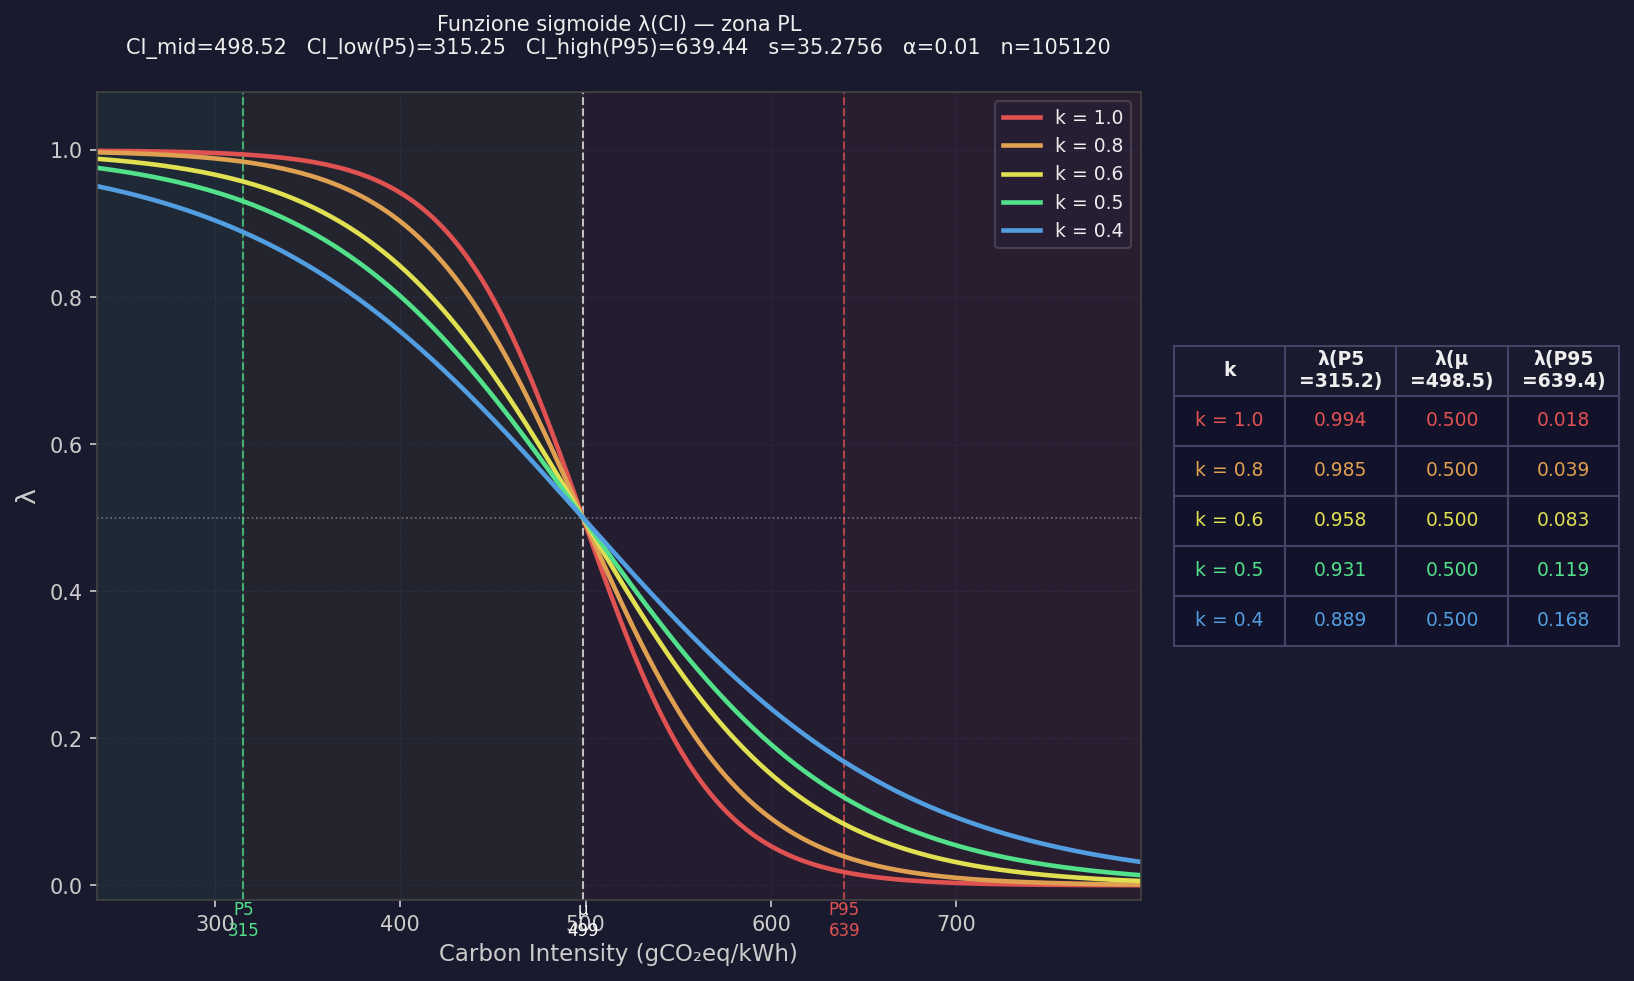
\includegraphics[width=\textwidth]{figures/lambda_curve_PL.png}
        \caption{Polonia (PL)}
    \end{subfigure}
    \caption{Esempi di sigmoidi locali utilizzate nell'Esperimento~2 per
             trasformare la carbon intensity oraria nel parametro
             $\lambda$. Francia e Polonia rappresentano due estremi della
             distribuzione osservata: la stessa funzione decisionale viene
             traslata e scalata rispetto ai valori tipici della zona. Il
             parametro $k$ controlla la rapidità della transizione: valori
             più alti rendono più brusco il passaggio da $\lambda \approx 1$
             a $\lambda \approx 0$, mentre valori più bassi producono una
             variazione più graduale.}
    \label{fig:exp2-sigmoidi-locali}
\end{figure}

Nei due esempi della Figura~\ref{fig:exp2-sigmoidi-locali}, il punto medio
della sigmoide coincide con la media storica locale: per la Francia la
transizione avviene a valori assoluti di CI molto bassi, mentre per la
Polonia la stessa logica decisionale è centrata su valori molto più elevati.
Questa differenza evidenzia il ruolo della calibrazione locale: $\lambda$
non misura quanto una CI sia alta in senso assoluto, ma quanto sia alta
rispetto al comportamento usuale della zona considerata.

Rispetto all'Esperimento~1, l'analisi include una metrica aggiuntiva:
l'emissione stimata di CO\textsubscript{2} per invocazione, calcolata
moltiplicando l'energia dell'invocazione per la carbon intensity corrente
della zona:
%
\begin{equation}
    \mathrm{CO_2}(r) =
        \frac{E(r)}{3{,}6 \cdot 10^6}
        \cdot \mathrm{CI}(r)
    \label{eq:emissioni-invocazione}
\end{equation}
%
dove $E(r)$ è l'energia dell'invocazione $r$ espressa in joule e
$\mathrm{CI}(r)$ è la carbon intensity corrente in
gCO\textsubscript{2}eq/kWh. Il fattore $3{,}6 \cdot 10^6$ converte
l'energia da joule a kWh, poiché $1~\mathrm{kWh}=3{,}6 \cdot 10^6~\mathrm{J}$.

%In questo esperimento l'attenzione si sposta dalle sole quote di selezione
%alle metriche aggregate: energia totale, emissioni totali e tempo medio di
%esecuzione. Per ciascuna zona viene calcolato il delta percentuale dello
%scheduler carbon-aware rispetto ad \emph{always-accurate}:
%%
%\begin{equation}
%    \Delta_{\mathrm{CO_2}} =
%        \frac{\mathrm{CO_2}_{\mathrm{accurate}} -
%              \mathrm{CO_2}_{\mathrm{carbon}}}
%             {\mathrm{CO_2}_{\mathrm{accurate}}}
%        \cdot 100
%    \label{eq:delta-co2}
%\end{equation}
%%
%e il costo qualitativo medio:
%%
%\begin{equation}
%    \Delta_Q =
%        \frac{Q_{\mathrm{accurate}} - Q_{\mathrm{carbon}}}
%             {Q_{\mathrm{accurate}}}
%        \cdot 100 .
%    \label{eq:delta-qualita}
%\end{equation}
%%
%Questi due indici sono sempre riportati congiuntamente, poiché una
%riduzione delle emissioni non può essere valutata correttamente senza
%quantificare il costo qualitativo che la accompagna.

\subsection{Risultati}
\label{subsec:esperimento2-risultati}

Come nell'Esperimento~1, il primo indicatore osservato è la distribuzione
delle varianti selezionate. Le Figure~\ref{fig:variant-distribution-numeric-exp2}
e~\ref{fig:variant-distribution-ml-exp2} riportano le quote di selezione
ottenute con calibrazione locale della CI.

Un primo segnale del corretto funzionamento dello scheduler è che le varianti
agli estremi della frontiera di Pareto --- quella a massima accuratezza e quella
a minima energia --- rimangono residuali in tutte le zone e per tutte le funzioni.
La sigmoide locale produce valori di $\lambda$ estremi solo quando il timestamp
è davvero anomalo rispetto alla storia della zona; la grande maggioranza dei
timestamp ordinari ricade in una regione intermedia, e lo scheduler converge
sulle varianti di compromesso. Le scelte estreme compaiono nei rari episodi di
picco o di minimo relativo della CI locale, non come comportamento sistematico.
La natura e la frequenza di questi episodi variano da zona a zona in funzione
della volatilità del mix energetico locale, e sono ciò che differenzia le
distribuzioni tra le cinque zone.

A differenza della calibrazione europea, $\lambda$ non misura il livello assoluto
di CI, ma quanto il timestamp si discosta dal profilo storico locale della rete:
anche una zona con CI media elevata produce $\lambda$ simili a quelli di una zona
più pulita quando il momento è ordinario per quella rete. La struttura zona per
zona delle distribuzioni riflette pertanto la forma del profilo storico di
ciascuna griglia.


\begin{figure}[p]
    \centering
    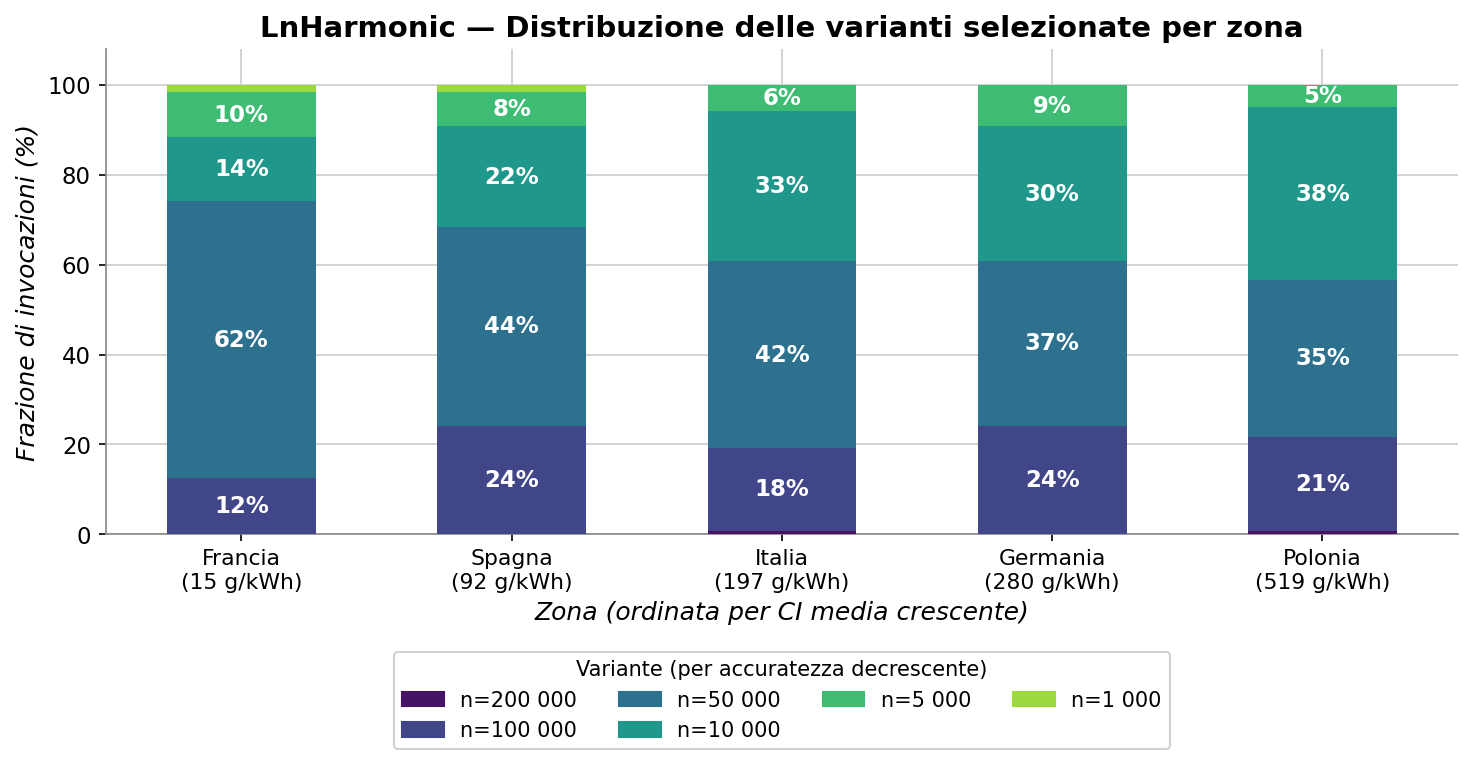
\includegraphics[width=0.72\textwidth]{figures/validation/exp2/01_variant_distribution_LnHarmonic.png}
    \vspace{0.2cm}
    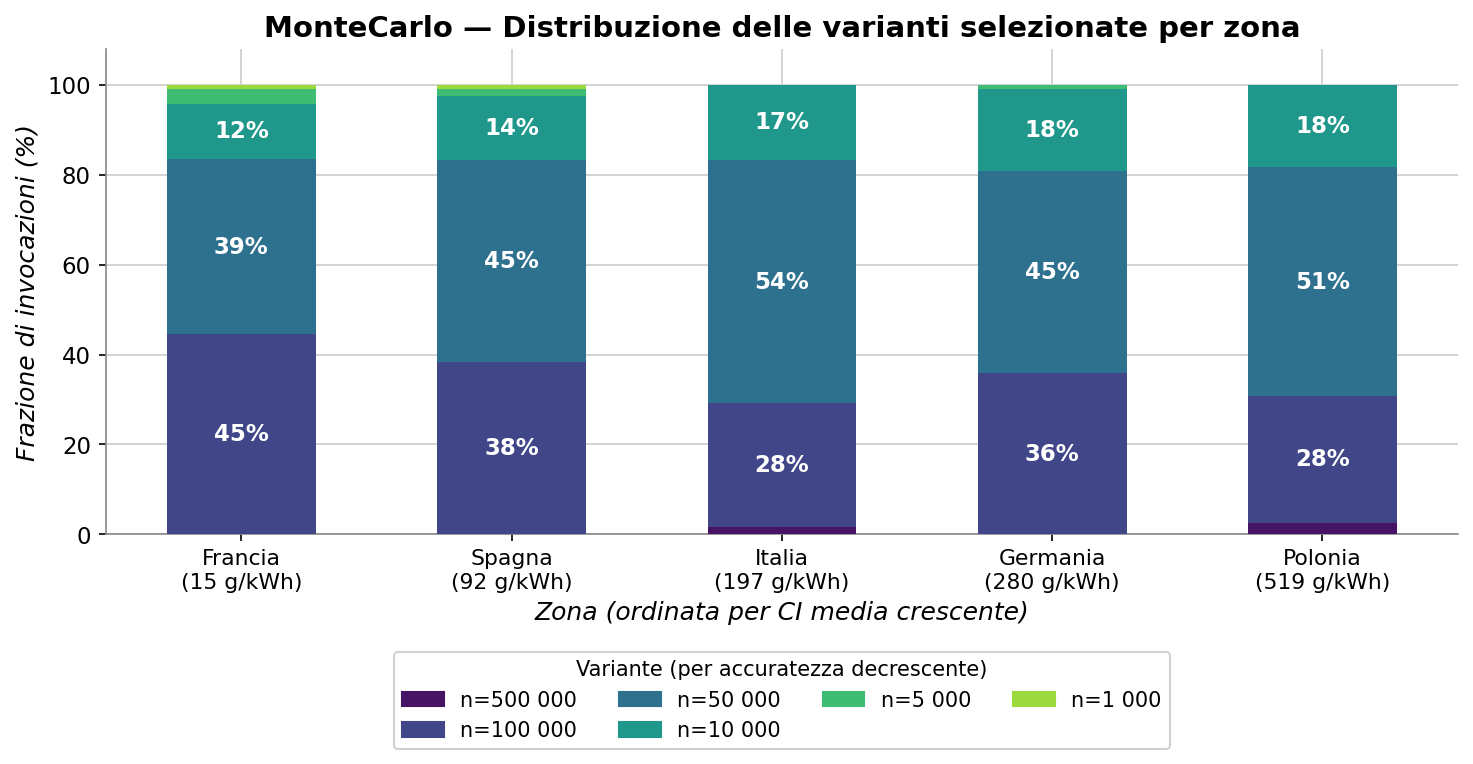
\includegraphics[width=0.72\textwidth]{figures/validation/exp2/01_variant_distribution_MonteCarlo.png}
    \vspace{0.2cm}
    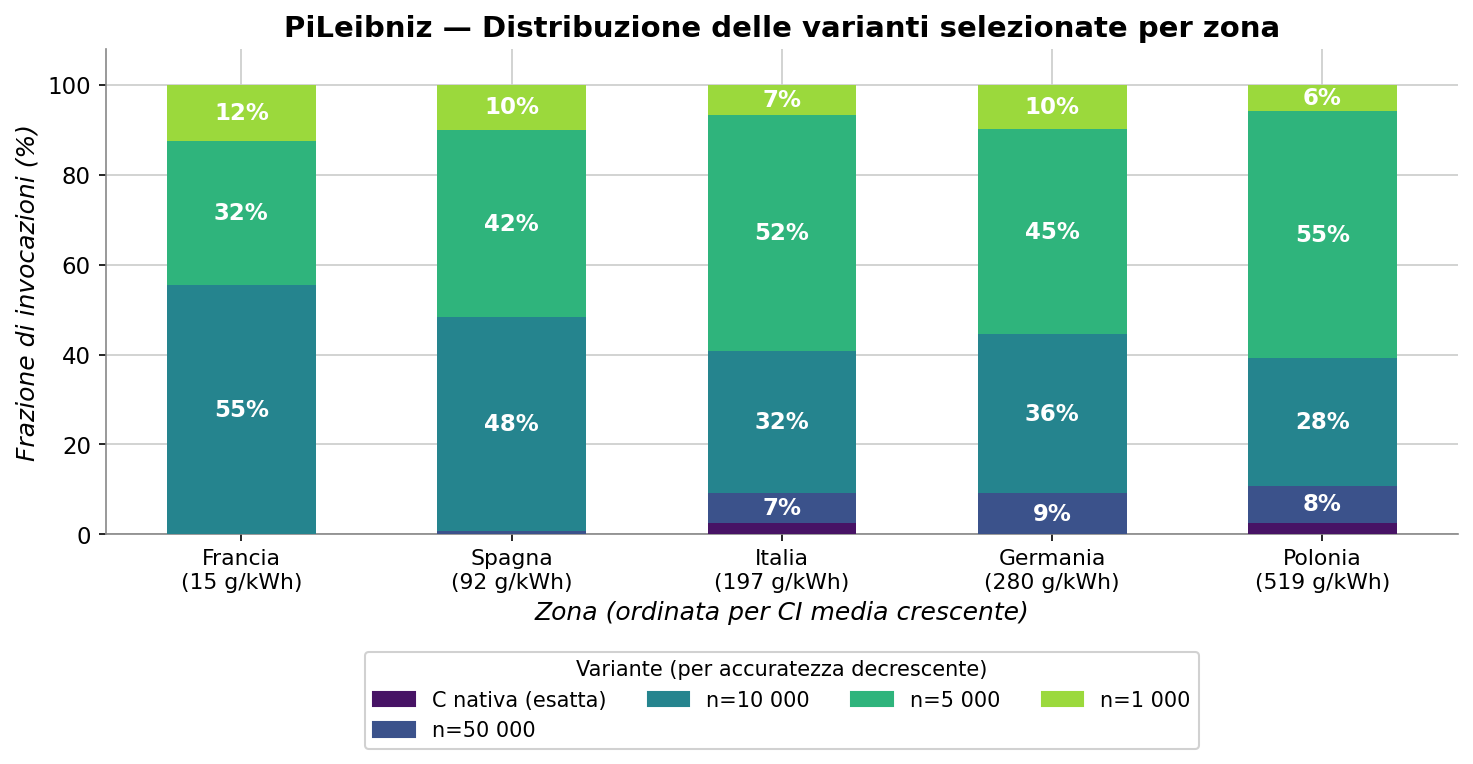
\includegraphics[width=0.72\textwidth]{figures/validation/exp2/01_variant_distribution_PiLeibniz.png}
    \caption{Distribuzione delle varianti selezionate per le funzioni
             numeriche nell'Esperimento~2. La calibrazione locale mantiene
             lo scheduler in una regione intermedia della frontiera: le
             varianti più efficienti crescono nei timestamp più sfavorevoli,
             ma le scelte non collassano sistematicamente sulla variante a
             energia minima.}
    \label{fig:variant-distribution-numeric-exp2}
\end{figure}

\begin{figure}[p]
    \centering
    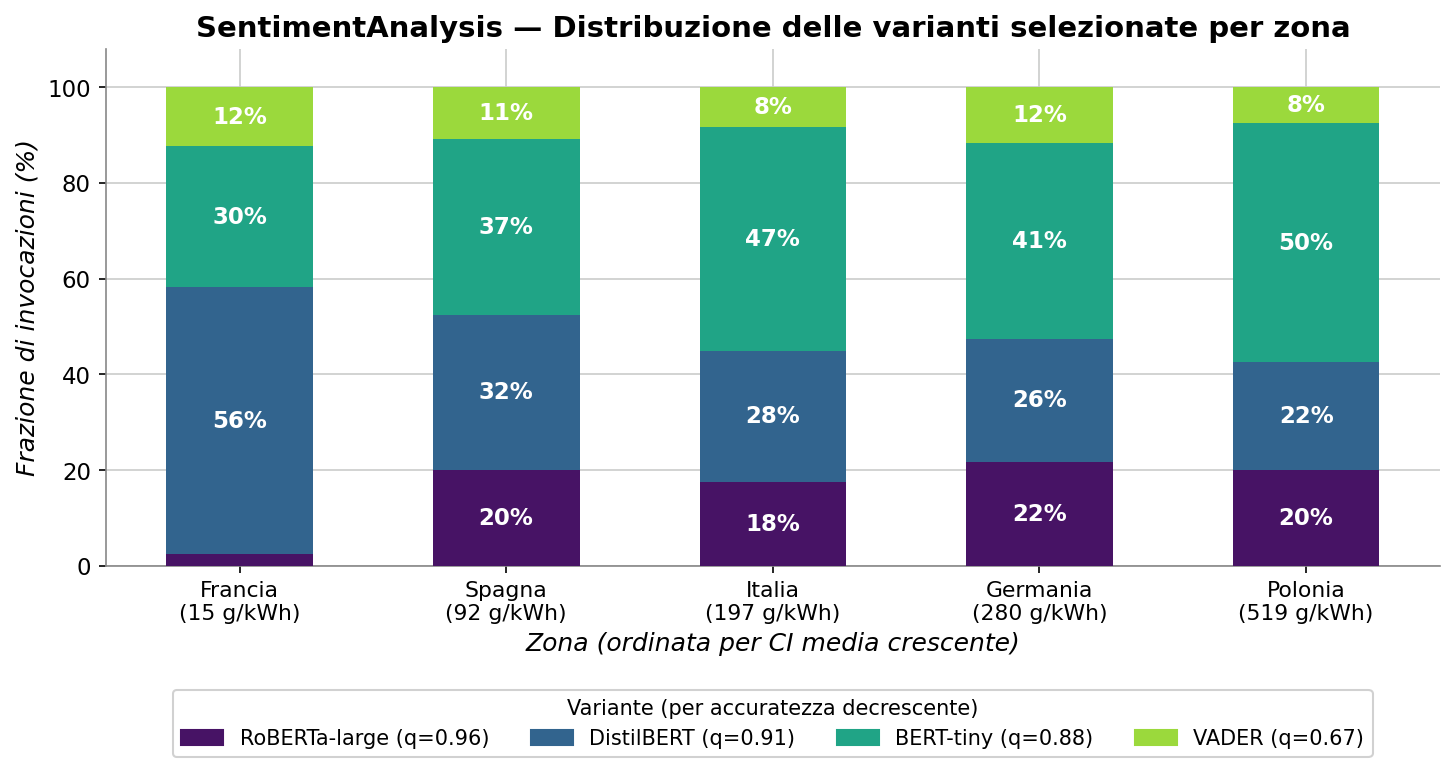
\includegraphics[width=0.72\textwidth]{figures/validation/exp2/01_variant_distribution_SentimentAnalysis.png}
    \vspace{0.2cm}
    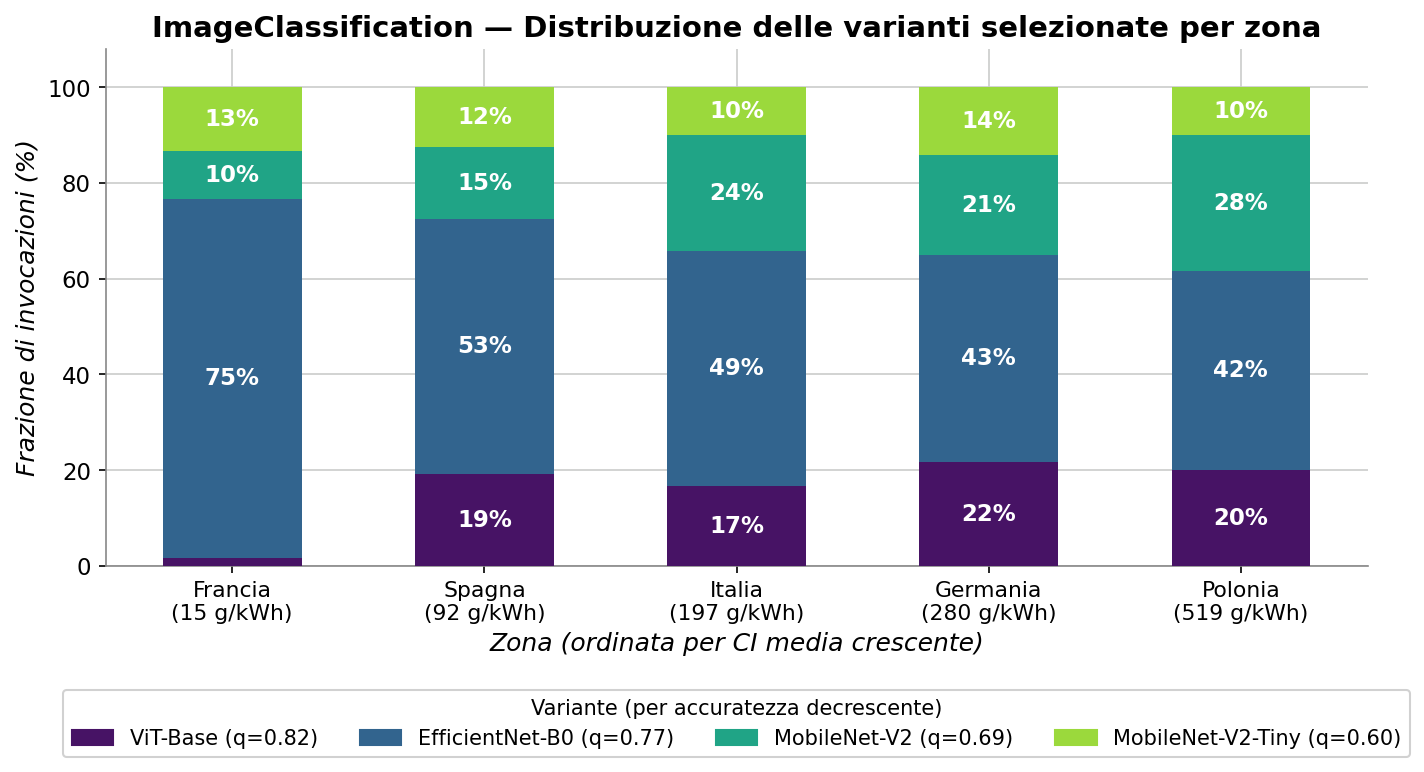
\includegraphics[width=0.72\textwidth]{figures/validation/exp2/01_variant_distribution_ImageClassification.png}
    \vspace{0.2cm}
    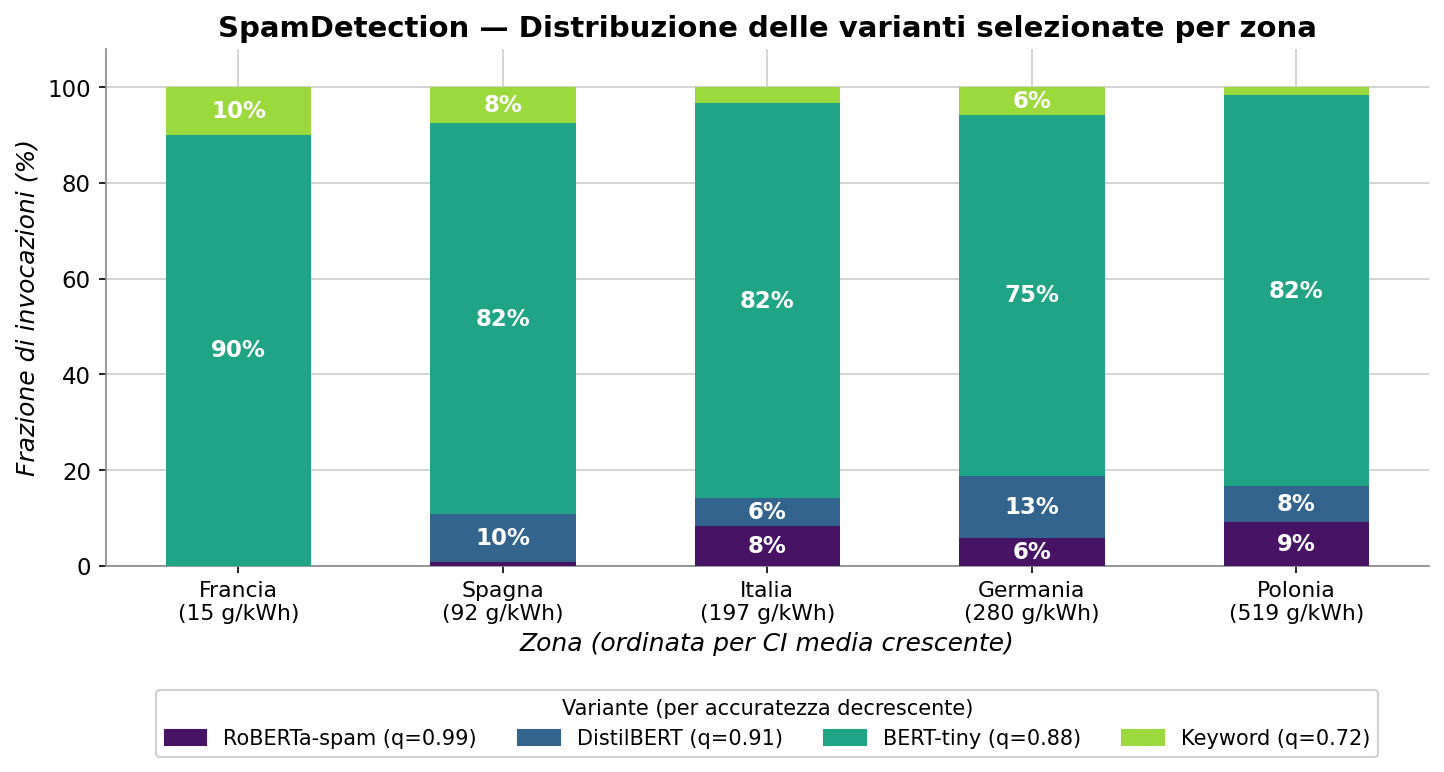
\includegraphics[width=0.72\textwidth]{figures/validation/exp2/01_variant_distribution_SpamDetection.png}
    \caption{Distribuzione delle varianti selezionate per le funzioni ML
             nell'Esperimento~2. Le transizioni sono discrete perché ogni
             variante corrisponde a un modello distinto; la calibrazione
             locale produce quindi combinazioni diverse di modelli nelle
             cinque zone, senza imporre una soglia globale unica.}
    \label{fig:variant-distribution-ml-exp2}
\end{figure}

\paragraph{Francia (15\,g/kWh).}
Francia è la zona con il profilo di CI più stabile, dominato dalla generazione
nucleare. La bassa volatilità si traduce in una distribuzione di $\lambda$ molto
concentrata attorno a valori medi, e lo scheduler converge quasi interamente
sull'unica variante intermedia principale: \texttt{n=50\,000} al 62\% in
LnHarmonic, \texttt{n=100\,000} al 45\% in MonteCarlo, \texttt{n=10\,000} al
55\% in PiLeibniz; nelle funzioni ML, EfficientNet-B0 al 75\% in
ImageClassification, DistilBERT al 56\% in SentimentAnalysis, BERT-tiny al
90\% in SpamDetection. Le varianti a massima accuratezza sono praticamente
assenti ($\leq 2$\%): la griglia francese opera già quasi sempre ai propri
valori minimi di CI, e non vi sono episodi di CI insolitamente bassa rispetto
alla norma locale. Le varianti a minima energia risultano invece più presenti
di quanto ci si aspetterebbe: in LnHarmonic e PiLeibniz raggiungono il 10\%
e il 12\%, rispettivamente, perché anche una griglia stabile presenta occasionali
fluttuazioni al rialzo della CI che, amplificate dalla calibrazione locale,
producono $\lambda$ sufficientemente elevati da attivare le varianti più leggere.

\paragraph{Spagna (92\,g/kWh).}
In Spagna il contributo di solare ed eolico introduce una volatilità maggiore
rispetto alla Francia. Il profilo di $\lambda$ è più disperso e le varianti
secondarie guadagnano peso. Per le funzioni numeriche la variante principale
rimane dominante (44\% in LnHarmonic, 45\% in MonteCarlo), ma crescono le quote
adiacenti: in LnHarmonic \texttt{n=10\,000} sale al 22\% e \texttt{n=100\,000}
al 24\%. Nelle funzioni ML emerge una quota non trascurabile delle varianti più
accurate --- ViT-Base al 19\% in ImageClassification, RoBERTa-large al 20\%
in SentimentAnalysis --- assente in Francia: la variabilità rinnovabile genera
episodi di CI insolitamente bassa rispetto alla media locale, e la calibrazione
li traduce in $\lambda$ minimi che attivano i modelli più pesanti.

\paragraph{Italia (197\,g/kWh).}
In Italia il baricentro si sposta verso varianti intermedie più leggere. In
LnHarmonic \texttt{n=10\,000} sale al 33\%, avvicinandosi alla quota della
variante principale \texttt{n=50\,000} (42\%); in PiLeibniz è \texttt{n=5\,000}
a dominare con il 52\%, mentre \texttt{n=50\,000} compare per la prima volta
in modo non residuale (7\%), segnale che alcuni timestamp producono $\lambda$
abbastanza bassi da spingere lo scheduler verso la regione più accurata della
frontiera. Anche
per le funzioni ML la struttura bimodale di Spagna si conferma: ViT-Base al
17\% e RoBERTa-large al 18\%, mentre le varianti a minima energia restano
contenute (7--10\%).

\paragraph{Germania (280\,g/kWh).}
Germania presenta la distribuzione più ampia tra le cinque zone. In
ImageClassification ViT-Base raggiunge il 22\%, il valore più alto dell'intero
esperimento: nonostante la CI media sia elevata, la griglia tedesca alterna tra
generazione rinnovabile (eolico) e fossile, producendo oscillazioni ampie che la
calibrazione locale registra come episodi di $\lambda$ sia molto bassi (CI
insolitamente pulita) sia molto alti (CI insolitamente elevata). Il risultato è
una distribuzione allargata verso entrambi gli estremi: \texttt{n=10\,000} al
30\% e MobileNet-V2 al 21\% nei timestamp più pesanti; ViT-Base e RoBERTa-large
nei momenti insolitamente puliti. La variante a minima energia rimane comunque
residuale (9\% in LnHarmonic, 6--14\% nelle funzioni ML).

\paragraph{Polonia (519\,g/kWh).}
Polonia, con la CI media più alta (519\,g/kWh), mostra la distribuzione più
spostata verso le varianti intermedie leggere: \texttt{n=10\,000} al 38\% in
LnHarmonic, \texttt{n=5\,000} al 55\% in PiLeibniz, BERT-tiny al 50\% in
SentimentAnalysis. Tuttavia, anche Polonia mantiene presenze significative delle
varianti più accurate (ViT-Base al 20\%, RoBERTa-large al 20\%), confermando
che nemmeno la zona più carbon-intensive produce $\lambda$ costantemente alti:
le ore notturne o i weekend abbassano periodicamente la CI sotto la norma locale,
generando episodi di $\lambda$ bassi. Specularmente, la variante a minima energia
è più contenuta rispetto alle attese (5--6\% nelle funzioni numeriche,
ad esempio LnHarmonic al 5\% e PiLeibniz al 6\%): la CI alta
è la norma polacca, non un picco, e la calibrazione locale non la interpreta come
evento eccezionale.

\paragraph{Trade-off energia--qualità.}
Le Figure~\ref{fig:tradeoff-numeric-exp2} e~\ref{fig:tradeoff-ml-exp2}
riportano il trade-off aggregato tra energia media per invocazione e qualità
media. In tutte le funzioni e in tutte le zone lo scheduler carbon-aware
rimane tra \emph{always-accurate} e \emph{always-energy}: riduce l'energia
rispetto alla baseline accurata e mantiene una qualità superiore alla
baseline energetica. Questo risultato è coerente con la distribuzione
empirica di $\lambda$: i timestamp con CI davvero anomala rispetto alla storia
locale sono rari, e la maggior parte delle invocazioni ricade in una regione
intermedia che produce un punto di operazione lontano da entrambi gli estremi.

\begin{figure}[p]
    \centering
    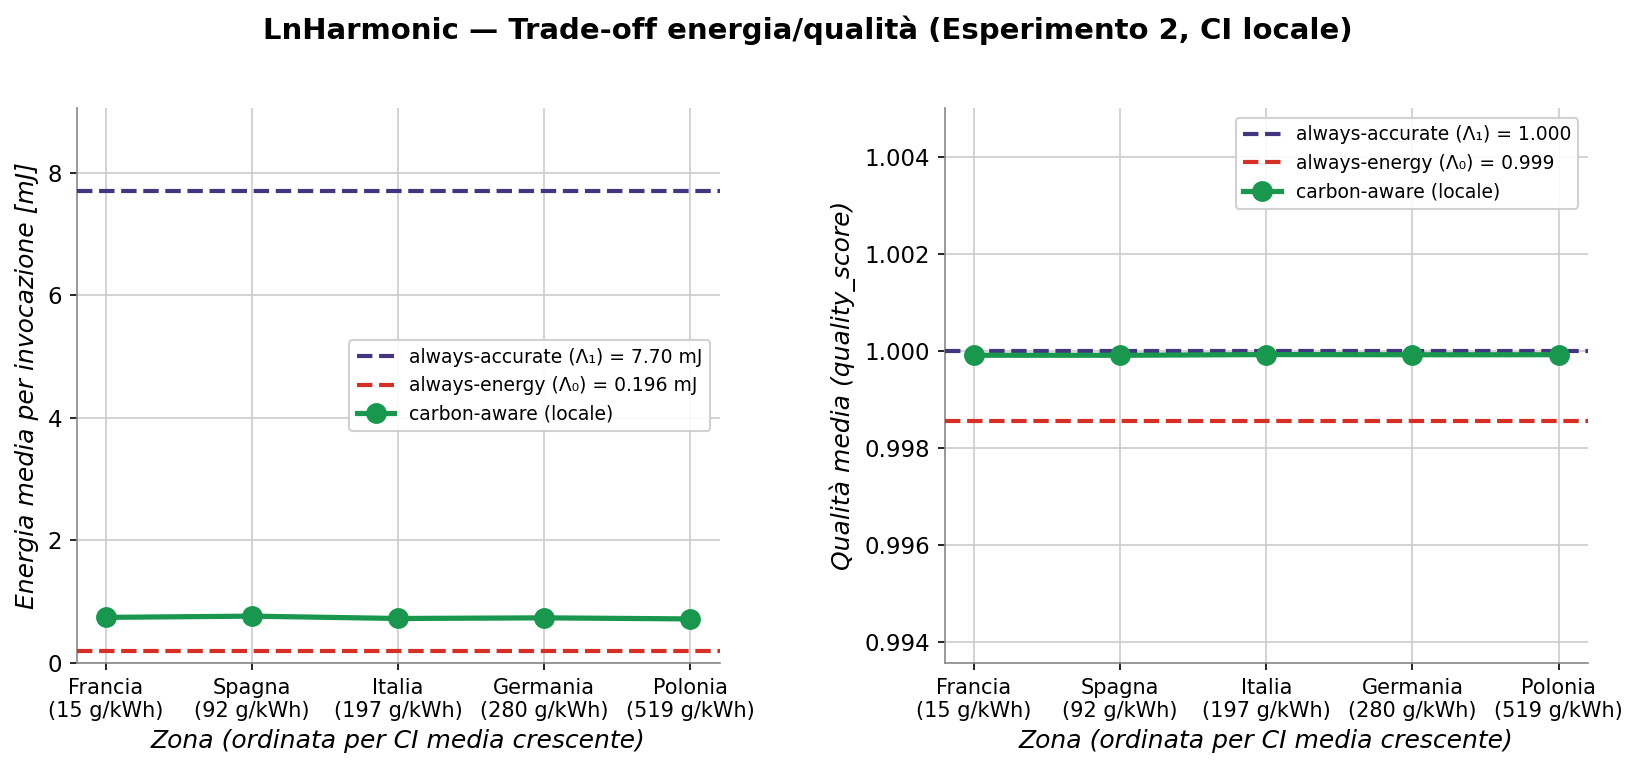
\includegraphics[width=0.78\textwidth]{figures/validation/exp2/03_tradeoff_LnHarmonic.png}
    \vspace{0.2cm}
    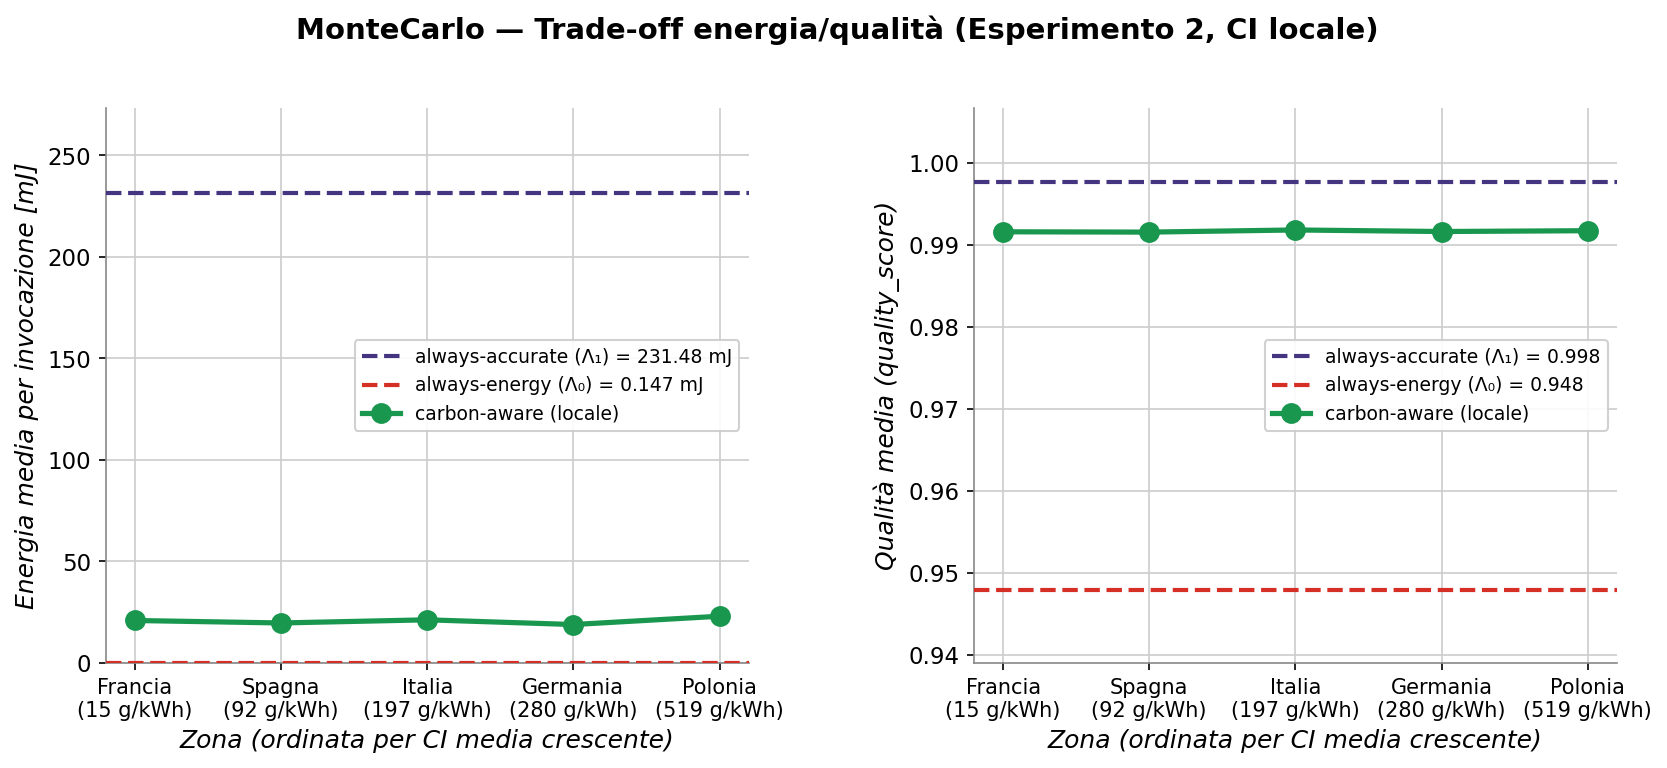
\includegraphics[width=0.78\textwidth]{figures/validation/exp2/03_tradeoff_MonteCarlo.png}
    \vspace{0.2cm}
    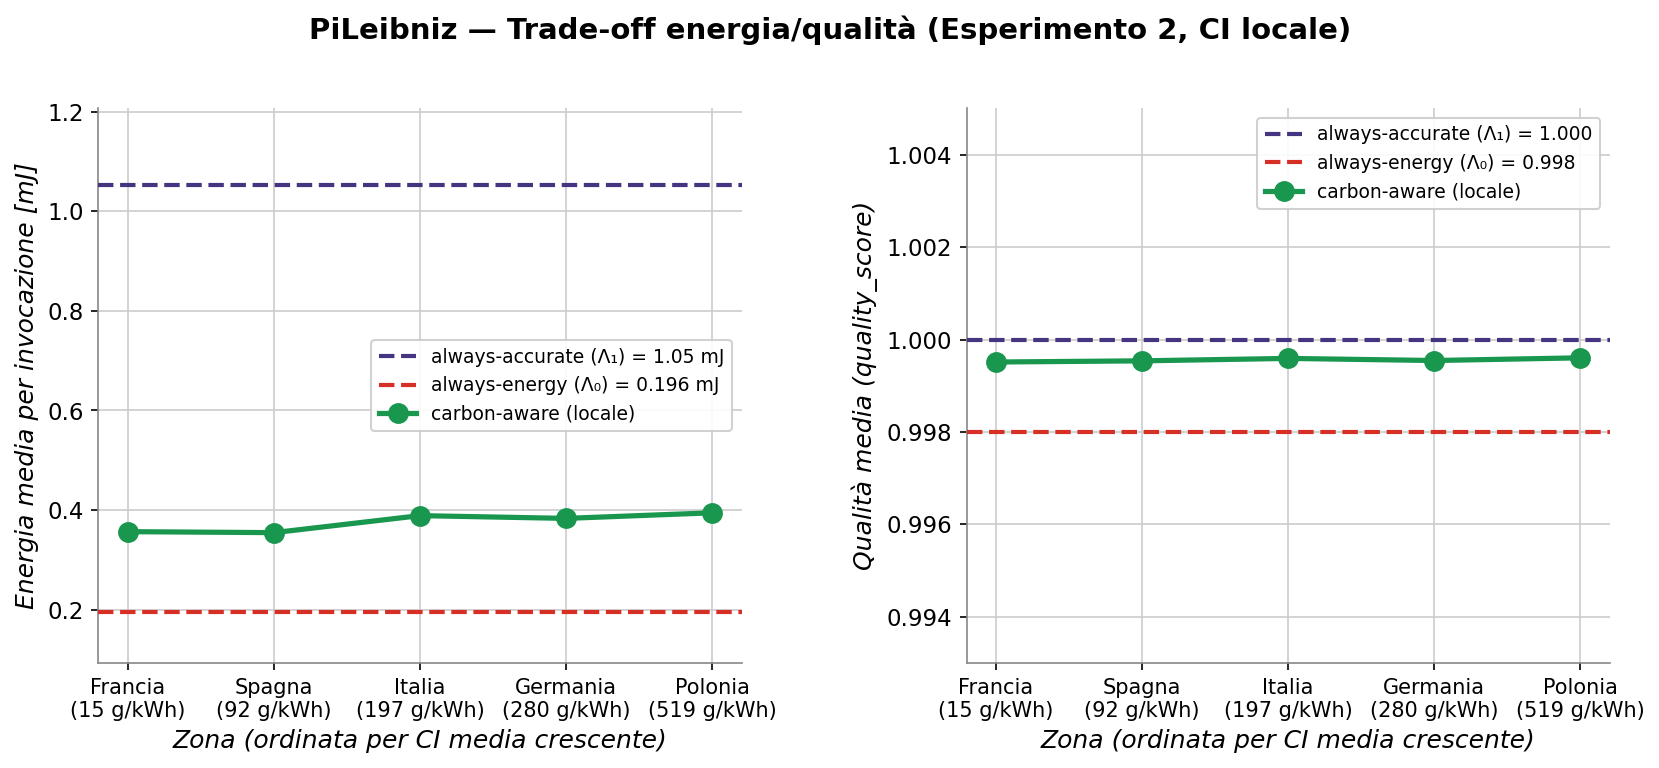
\includegraphics[width=0.78\textwidth]{figures/validation/exp2/03_tradeoff_PiLeibniz.png}
    \caption{Trade-off energia--qualità per le funzioni numeriche
             nell'Esperimento~2. Il costo qualitativo resta molto contenuto:
             le curve di qualità sono quasi sovrapposte alla baseline
             accurata, mentre l'energia media si riduce sensibilmente.}
    \label{fig:tradeoff-numeric-exp2}
\end{figure}

\begin{figure}[p]
    \centering
    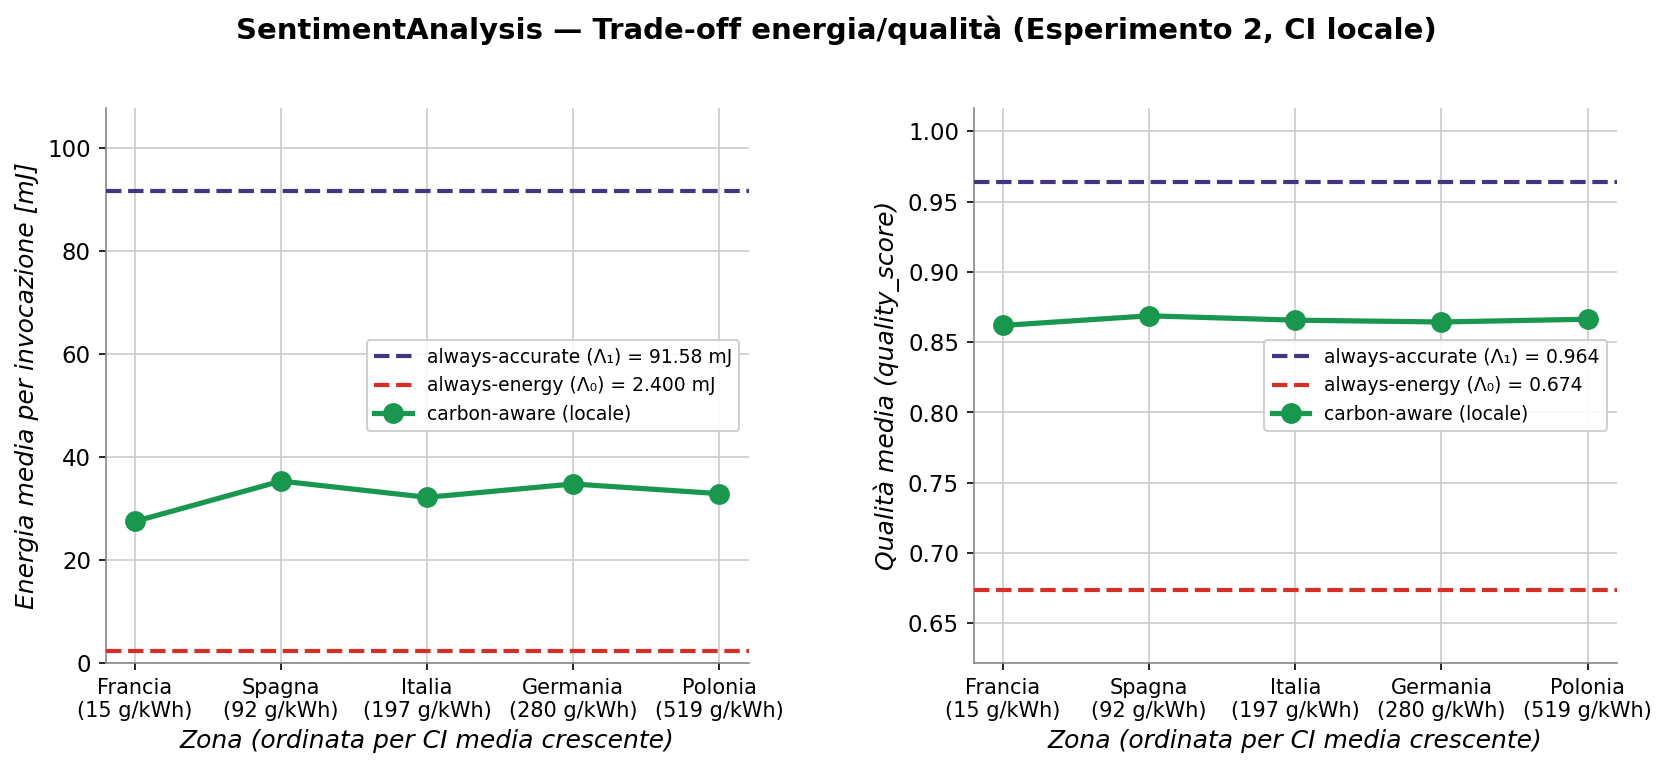
\includegraphics[width=0.78\textwidth]{figures/validation/exp2/03_tradeoff_SentimentAnalysis.png}
    \vspace{0.2cm}
    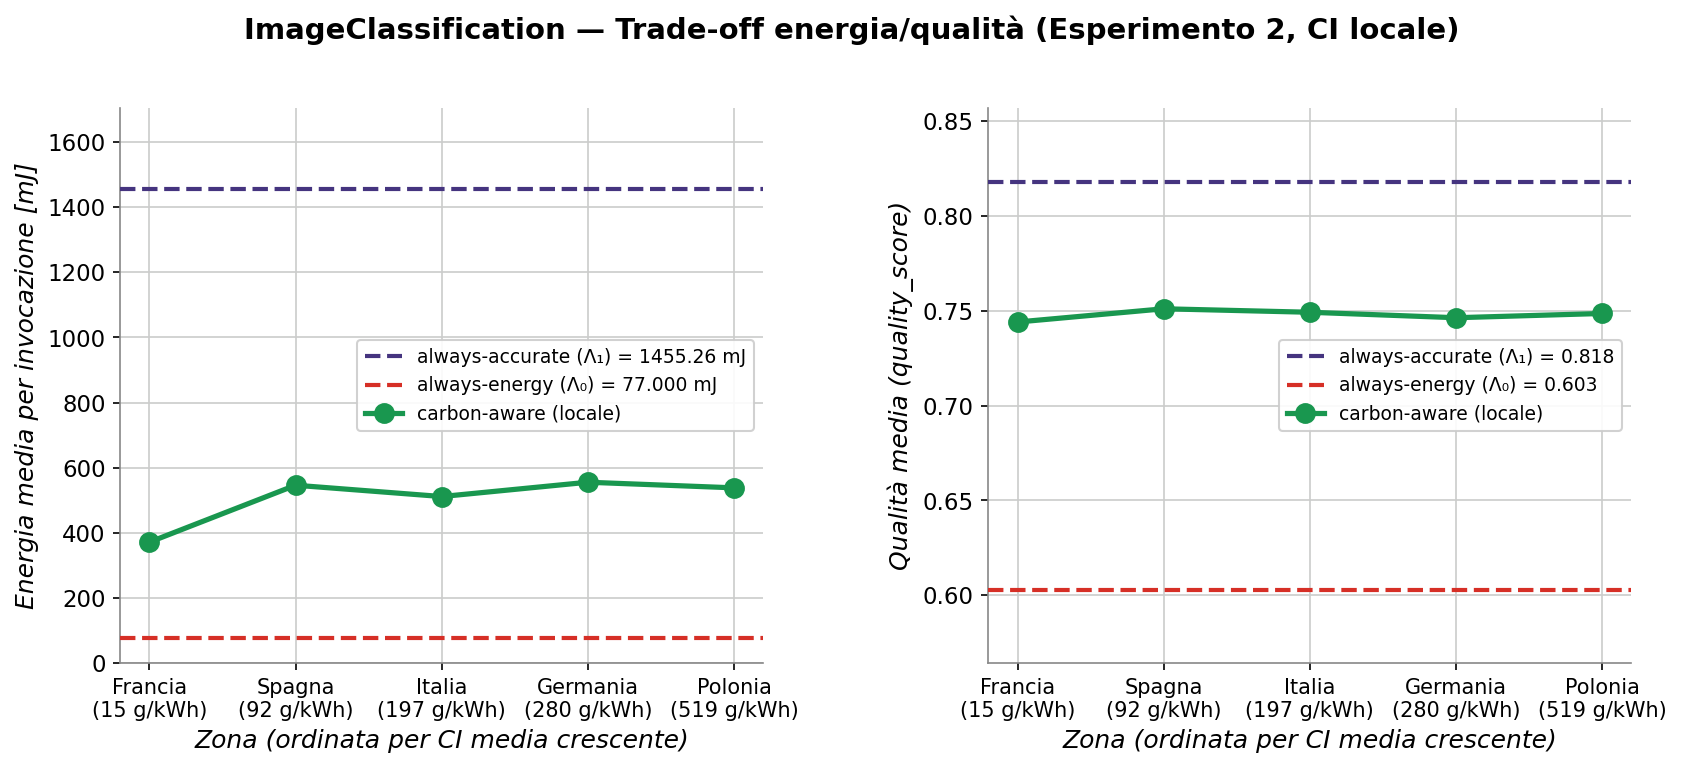
\includegraphics[width=0.78\textwidth]{figures/validation/exp2/03_tradeoff_ImageClassification.png}
    \vspace{0.2cm}
    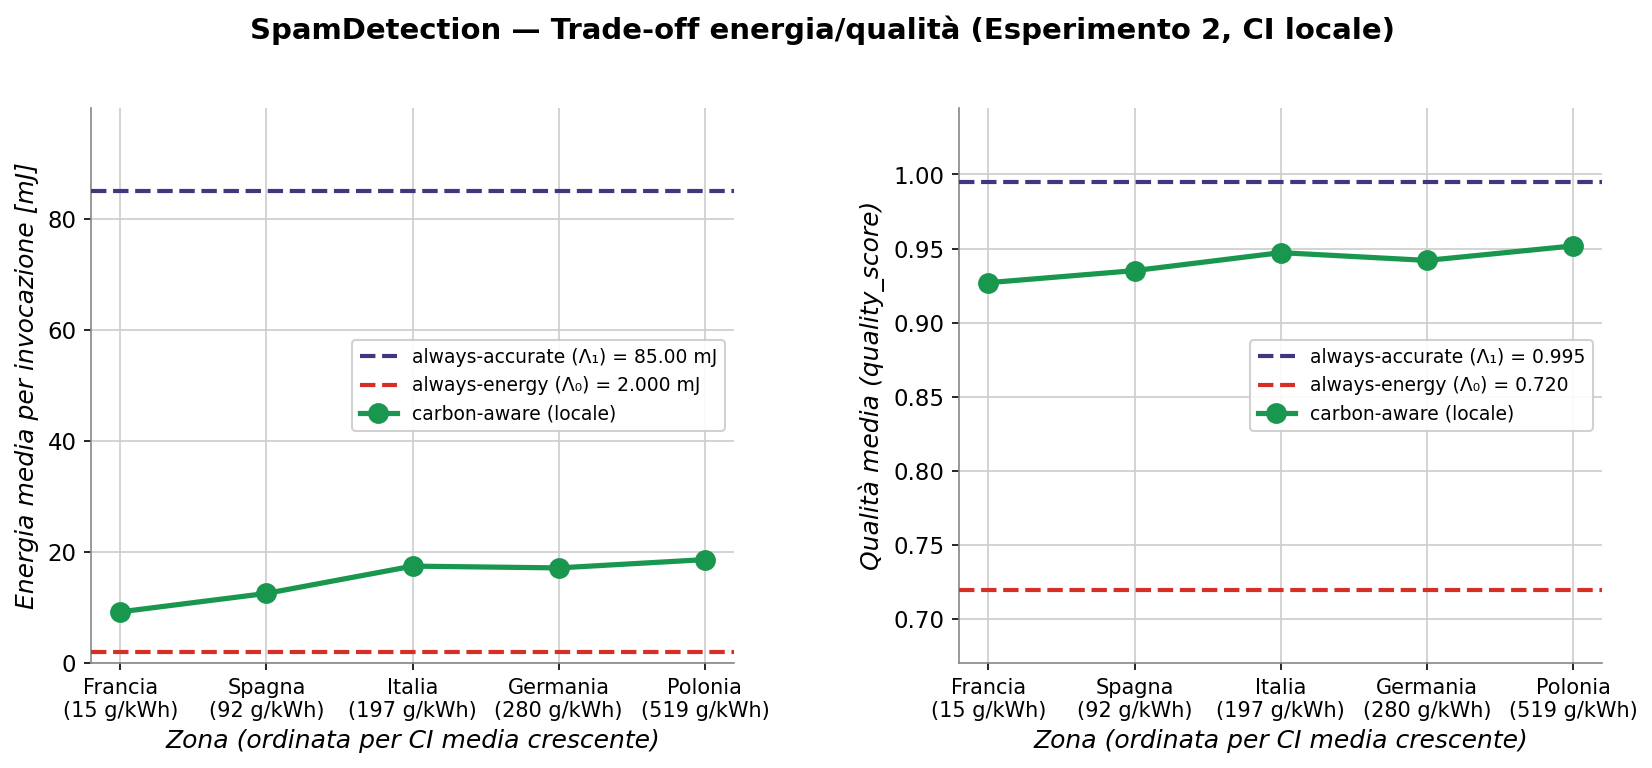
\includegraphics[width=0.78\textwidth]{figures/validation/exp2/03_tradeoff_SpamDetection.png}
    \caption{Trade-off energia--qualità per le funzioni ML nell'Esperimento~2.
             Il risparmio energetico è accompagnato da un costo qualitativo
             più visibile rispetto alle funzioni numeriche, perché il passaggio
             tra modelli produce salti discreti di accuratezza.}
    \label{fig:tradeoff-ml-exp2}
\end{figure}

Il comportamento delle curve conferma la differenza strutturale tra funzioni
numeriche e ML\@. LnHarmonic e PiLeibniz mantengono qualità praticamente identiche
a 1 anche quando l'energia si riduce rispettivamente di circa il 90\% e il 63\%
rispetto alla baseline accurata: la frontiera continua permette di spostarsi
verso varianti meno costose senza attraversare salti qualitativi rilevanti.
MonteCarlo mostra una perdita leggermente più visibile
($\Delta Q_{acc} \approx -0.7$\%), ma rimane prossimo alla qualità massima.

Per le funzioni ML il costo qualitativo è più evidente: ImageClassification
opera tra 0.74 e 0.75 (vs 0.818 della baseline accurata e 0.603 di quella
energetica), SentimentAnalysis tra 0.86 e 0.87 (vs 0.964 e 0.674),
SpamDetection tra 0.93 e 0.95 (vs 0.995 e 0.720). Il degrado non dipende
dalla zona --- la qualità è sostanzialmente stabile su tutte e cinque le zone
per ciascuna funzione --- ma dalla granularità della frontiera: i salti discreti
di accuratezza tra modelli adiacenti rendono il costo qualitativo inevitabilmente
più visibile rispetto alle funzioni numeriche.

Merita osservare la variazione di energia tra zone nelle funzioni ML\@.
In ImageClassification Francia produce in media circa 370\,mJ per invocazione,
mentre le altre zone oscillano tra 510 e 560\,mJ; la differenza non riflette
la CI locale (la calibrazione è relativa), ma il mix di varianti selezionate ---
in Francia ViT-Base è quasi assente (2\%, 1455\,mJ), mentre nelle altre zone
raggiunge il 17--22\%. Analogamente, SentimentAnalysis in Francia consuma circa
28\,mJ contro i 32--35\,mJ delle altre zone, dove la presenza di RoBERTa-large
(91\,mJ) è più significativa. La calibrazione locale non converge quindi sulla
stessa composizione energetica in tutte le zone.

La Tabella~\ref{tab:baseline-comparison-exp2} quantifica gli stessi fenomeni
rispetto alle due baseline. La colonna $\Delta \mathrm{CO_2}$ combina il
profilo energetico della variante con la CI del timestamp: quando lo scheduler
seleziona varianti più efficienti nei momenti localmente più sfavorevoli, il
beneficio carbonico risulta sistematicamente più marcato del solo risparmio
energetico medio, come si osserva in tutte le funzioni e tutte le zone.

\begin{table}[p]
    \centering
    \caption{Variazione percentuale dello scheduler carbon-aware
             dell'Esperimento~2 rispetto alle due baseline. $\Delta E$,
             $\Delta \mathrm{CO_2}$, $\Delta T$ e $\Delta Q$ sono calcolati
             sulle medie per invocazione. Valori negativi di $\Delta E$,
             $\Delta \mathrm{CO_2}$ e $\Delta T$ indicano un risparmio
             rispetto alla baseline; valori positivi di $\Delta Q$ indicano
             qualità superiore alla baseline.}
    \label{tab:baseline-comparison-exp2}
    \resizebox{\textwidth}{!}{%
    \begin{tabular}{llrrrrrrrr}
        \toprule
        Funzione & Zona
            & $\Delta E_{acc}$ & $\Delta \mathrm{CO_2}_{acc}$
            & $\Delta T_{acc}$ & $\Delta Q_{acc}$
            & $\Delta E_{ene}$ & $\Delta \mathrm{CO_2}_{ene}$
            & $\Delta T_{ene}$ & $\Delta Q_{ene}$ \\
        \midrule
        PiLeibniz & Francia
            & \greenval{-66.15\%} & \greenval{-71.89\%} & \greenval{-71.68\%} & \redval{-0.05\%} & \redval{+81.71\%} & \redval{+50.85\%} & \redval{+10.94\%} & \greenval{+0.15\%} \\
                  & Spagna
            & \greenval{-66.28\%} & \greenval{-69.44\%} & \greenval{-23.27\%} & \redval{-0.05\%} & \redval{+80.98\%} & \redval{+64.02\%} & \redval{+13.58\%} & \greenval{+0.15\%} \\
                  & Italia
            & \greenval{-63.04\%} & \greenval{-66.51\%} & \greenval{-15.19\%} & \redval{-0.04\%} & \redval{+98.39\%} & \redval{+79.77\%} & \redval{+26.73\%} & \greenval{+0.16\%} \\
                  & Germania
            & \greenval{-63.91\%} & \greenval{-68.41\%} & \greenval{-14.75\%} & \redval{-0.05\%} & \redval{+93.73\%} & \redval{+69.56\%} & \redval{+28.40\%} & \greenval{+0.15\%} \\
                  & Polonia
            & \greenval{-62.50\%} & \greenval{-65.26\%} & \greenval{-13.46\%} & \redval{-0.04\%} & \redval{+101.28\%} & \redval{+86.47\%} & \redval{+27.79\%} & \greenval{+0.16\%} \\
        \midrule
        LnHarmonic & Francia
            & \greenval{-90.35\%} & \greenval{-92.73\%} & \greenval{-89.15\%} & \redval{-0.01\%} & \redval{+279.03\%} & \redval{+185.79\%} & \redval{+96.77\%} & \greenval{+0.14\%} \\
                   & Spagna
            & \greenval{-90.09\%} & \greenval{-91.68\%} & \greenval{-88.56\%} & \redval{-0.01\%} & \redval{+289.28\%} & \redval{+226.98\%} & \redval{+114.24\%} & \greenval{+0.13\%} \\
                   & Italia
            & \greenval{-90.59\%} & \greenval{-91.51\%} & \greenval{-89.64\%} & \redval{-0.01\%} & \redval{+269.75\%} & \redval{+233.71\%} & \redval{+95.15\%} & \greenval{+0.14\%} \\
                   & Germania
            & \greenval{-90.45\%} & \greenval{-91.94\%} & \greenval{-89.14\%} & \redval{-0.01\%} & \redval{+275.08\%} & \redval{+216.57\%} & \redval{+98.91\%} & \greenval{+0.14\%} \\
                   & Polonia
            & \greenval{-90.68\%} & \greenval{-91.40\%} & \greenval{-89.47\%} & \redval{-0.01\%} & \redval{+266.23\%} & \redval{+237.83\%} & \redval{+94.62\%} & \greenval{+0.14\%} \\
        \midrule
        MonteCarlo & Francia
            & \greenval{-91.02\%} & \greenval{-94.82\%} & \greenval{-82.14\%} & \redval{-0.61\%} & \redval{+14034.02\%} & \redval{+8059.95\%} & \redval{+450.04\%} & \greenval{+4.60\%} \\
                   & Spagna
            & \greenval{-91.51\%} & \greenval{-93.58\%} & \greenval{-83.07\%} & \redval{-0.61\%} & \redval{+13276.69\%} & \redval{+10012.13\%} & \redval{+430.90\%} & \greenval{+4.59\%} \\
                   & Italia
            & \greenval{-90.83\%} & \greenval{-92.86\%} & \greenval{-82.64\%} & \redval{-0.59\%} & \redval{+14332.33\%} & \redval{+11147.43\%} & \redval{+446.52\%} & \greenval{+4.62\%} \\
                   & Germania
            & \greenval{-91.84\%} & \greenval{-93.74\%} & \greenval{-83.49\%} & \redval{-0.61\%} & \redval{+12754.73\%} & \redval{+9755.88\%} & \redval{+414.82\%} & \greenval{+4.60\%} \\
                   & Polonia
            & \greenval{-90.07\%} & \greenval{-91.91\%} & \greenval{-82.08\%} & \redval{-0.60\%} & \redval{+15534.17\%} & \redval{+12636.41\%} & \redval{+467.06\%} & \greenval{+4.61\%} \\
        \midrule
        SentimentAnalysis & Francia
            & \greenval{-69.73\%} & \greenval{-82.52\%} & \greenval{-78.36\%} & \redval{-10.55\%} & \redval{+1055.05\%} & \redval{+567.10\%} & \redval{+531.03\%} & \greenval{+27.94\%} \\
                          & Spagna
            & \greenval{-61.46\%} & \greenval{-73.61\%} & \greenval{-71.24\%} & \redval{-9.89\%} & \redval{+1370.69\%} & \redval{+907.01\%} & \redval{+772.25\%} & \greenval{+28.89\%} \\
                          & Italia
            & \greenval{-64.90\%} & \greenval{-72.44\%} & \greenval{-74.01\%} & \redval{-10.21\%} & \redval{+1239.26\%} & \redval{+951.65\%} & \redval{+691.47\%} & \greenval{+28.43\%} \\
                          & Germania
            & \greenval{-62.07\%} & \greenval{-74.47\%} & \greenval{-71.85\%} & \redval{-10.34\%} & \redval{+1347.24\%} & \redval{+874.06\%} & \redval{+762.29\%} & \greenval{+28.24\%} \\
                          & Polonia
            & \greenval{-64.13\%} & \greenval{-70.17\%} & \greenval{-72.95\%} & \redval{-10.14\%} & \redval{+1268.89\%} & \redval{+1038.07\%} & \redval{+738.24\%} & \greenval{+28.53\%} \\
        \midrule
        SpamDetection & Francia
            & \greenval{-89.18\%} & \greenval{-91.03\%} & \greenval{-63.45\%} & \redval{-6.83\%} & \redval{+360.00\%} & \redval{+281.17\%} & \redval{+101.37\%} & \greenval{+28.75\%} \\
                      & Spagna
            & \greenval{-85.26\%} & \greenval{-88.09\%} & \greenval{-79.01\%} & \redval{-6.02\%} & \redval{+526.25\%} & \redval{+406.15\%} & \redval{+148.16\%} & \greenval{+29.88\%} \\
                      & Italia
            & \greenval{-79.48\%} & \greenval{-83.87\%} & \greenval{-72.62\%} & \redval{-4.80\%} & \redval{+772.08\%} & \redval{+585.39\%} & \redval{+235.59\%} & \greenval{+31.56\%} \\
                      & Germania
            & \greenval{-80.21\%} & \greenval{-85.71\%} & \greenval{-79.14\%} & \redval{-5.37\%} & \redval{+741.25\%} & \redval{+507.49\%} & \redval{+107.26\%} & \greenval{+30.77\%} \\
                      & Polonia
            & \greenval{-78.10\%} & \greenval{-81.69\%} & \greenval{-72.59\%} & \redval{-4.34\%} & \redval{+830.83\%} & \redval{+678.36\%} & \redval{+227.54\%} & \greenval{+32.19\%} \\
        \midrule
        ImageClassification & Francia
            & \greenval{-74.51\%} & \greenval{-81.80\%} & \greenval{-47.64\%} & \redval{-9.04\%} & \redval{+381.71\%} & \redval{+243.93\%} & \redval{+51.67\%} & \greenval{+23.40\%} \\
                            & Spagna
            & \greenval{-62.49\%} & \greenval{-72.69\%} & \greenval{-59.98\%} & \redval{-8.18\%} & \redval{+608.86\%} & \redval{+416.07\%} & \redval{+56.74\%} & \greenval{+24.55\%} \\
                            & Italia
            & \greenval{-64.88\%} & \greenval{-71.38\%} & \greenval{-61.84\%} & \redval{-8.41\%} & \redval{+563.75\%} & \redval{+440.84\%} & \redval{+42.06\%} & \greenval{+24.25\%} \\
                            & Germania
            & \greenval{-61.86\%} & \greenval{-72.97\%} & \greenval{-60.05\%} & \redval{-8.76\%} & \redval{+620.84\%} & \redval{+410.91\%} & \redval{+51.99\%} & \greenval{+23.77\%} \\
                            & Polonia
            & \greenval{-63.05\%} & \greenval{-68.51\%} & \greenval{-60.05\%} & \redval{-8.49\%} & \redval{+598.43\%} & \redval{+495.12\%} & \redval{+54.14\%} & \greenval{+24.14\%} \\
        \bottomrule
    \end{tabular}
    }
\end{table}

\subsection{Interpretazione}
\label{subsec:esperimento2-interpretazione}

L'Esperimento~2 mostra come le decisioni cambiano quando la CI viene
interpretata rispetto al contesto locale anziché rispetto a una scala
europea uniforme. Rispetto a \emph{always-accurate}, lo scheduler riduce
sempre energia e CO\textsubscript{2} in tutte le zone e funzioni osservate.
Il risparmio carbonico è sistematicamente più alto del risparmio energetico:
la scelta della variante non è indipendente dalla CI del timestamp, e lo
scheduler tende a selezionare varianti efficienti proprio nei momenti
localmente più sfavorevoli, amplificando il beneficio carbonico oltre il
solo risparmio energetico medio.

Il risparmio energetico è però intrinsecamente legato a un costo qualitativo:
selezionare varianti meno costose significa, per costruzione, scegliere
varianti meno accurate. Più lo scheduler si sposta verso varianti efficienti,
maggiore è la perdita di qualità che ne deriva. Il grado di questa correlazione
dipende dalla struttura della frontiera di Pareto di ciascuna funzione: quando
le varianti adiacenti differiscono poco in accuratezza, il costo qualitativo
per unità di risparmio energetico è contenuto; quando i salti sono ampi, anche
una piccola riduzione di energia può comportare una perdita qualitativa
visibile. Nelle funzioni numeriche la perdita rispetto ad \emph{always-accurate}
resta inferiore all'1\% nonostante riduzioni di energia dell'ordine del 60--90\%,
perché la frontiera continua permette compromessi fini. Nelle funzioni ML la
perdita è invece tra il 5\% e l'11\%, riflettendo i salti discreti tra modelli
adiacenti: ImageClassification e SentimentAnalysis perdono circa 8--11\%, mentre
SpamDetection, pur risparmiando più energia, perde solo il 5--7\% perché BERT-tiny
(dominante) è qualitativamente più vicino a RoBERTa-spam di quanto VADER non
lo sia rispetto ai modelli neurali di SentimentAnalysis.

Il confronto con \emph{always-energy} conferma che lo scheduler non minimizza
semplicemente l'energia: consuma più della baseline energetica, ma mantiene
una qualità nettamente superiore in tutte le funzioni. Questo comportamento
è la conseguenza diretta della calibrazione locale: la sigmoide non classifica
una zona come ``pulita'' o ``carbon-intensive'' in senso assoluto, ma valuta
ogni timestamp rispetto alla storia specifica della rete. Di conseguenza, anche
in Polonia compaiono scelte non estreme quando la CI è bassa rispetto al
profilo locale, e in Francia possono essere selezionate varianti efficienti
nei rari momenti di CI relativamente alta.


% -----------------------------------------------------------
\section{Esperimento 3: valutazione energetica e stabilità operativa}
\label{sec:esperimento3}
% -----------------------------------------------------------

\subsection{Obiettivo e struttura}
\label{subsec:esperimento3-obiettivo}

Il terzo esperimento valuta lo scheduler carbon-aware lungo due dimensioni
complementari che gli Esperimenti~1 e~2 non affrontano direttamente.

La prima dimensione riguarda il \emph{confronto quantitativo} tra le tre
policy in termini di energia consumata, emissioni di
CO\textsubscript{2} e qualità del risultato in condizioni di carico
variabile ma moderato. Negli Esperimenti~1 e~2 le invocazioni sono
eseguite in modo sequenziale da un singolo thread: il tempo di risposta
coincide quindi per costruzione con il solo tempo di esecuzione della
variante, senza alcuna componente di attesa. L'Esperimento~3 introduce
un modello concorrente a tempo continuo e verifica che, in assenza di
saturazione, questa metrica resti interpretabile nello stesso modo: il
tempo di risposta deve ancora riflettere principalmente il peso
computazionale della variante scelta, non la pressione del carico.

La seconda dimensione riguarda la \emph{stabilità operativa} dello
scheduler sotto carico crescente fino a condizioni di stress. In un
deployment reale le richieste possono arrivare in burst; è necessario
verificare che la logica di selezione della variante non costituisca un
collo di bottiglia e che il sistema si comporti in modo prevedibile
quando il tasso di arrivo supera la soglia di saturazione.

Le due dimensioni sono valutate su due run distinti dello stesso
workload k6, differenziati esclusivamente dal profilo di carico:
%
\begin{itemize}
  \item \textbf{Run~A -- carico moderato}: il tasso di arrivo è
        mantenuto al di sotto della soglia di saturazione per tutte e
        tre le policy. Tutte le richieste vengono completate; il tempo
        di risposta osservato riflette il solo tempo di esecuzione.
        Questo run produce i dati per il confronto quantitativo di
        energia, CO\textsubscript{2}, qualità e latenza.
  \item \textbf{Run~B -- carico crescente}: il tasso di arrivo aumenta
        progressivamente fino a indurre saturazione nella policy
        $\lambda{=}1$. Questo run produce i dati per l'analisi della
        stabilità operativa e del comportamento dello scheduler sotto
        pressione.
\end{itemize}

Il workload è deterministico: a parità di seed, la sequenza di
richieste --- funzione invocata, zona geografica, valore di carbon
intensity --- è identica per tutte e tre le policy e tra i due run.
% -----------------------------------------------------------
\subsection{Prima parte: confronto energetico a carico moderato (Run~A)}
\label{subsec:esperimento3-parte1}
% -----------------------------------------------------------

\subsubsection{Configurazione}
\label{subsubsec:esperimento3-parte1-config}

Il Run~A utilizza un profilo di carico variabile ma contenuto, composto
dalle prime tre fasi del workload k6 (\emph{Low}, \emph{Medium},
\emph{High} a rispettivamente 2, 5 e 10~richieste al secondo), per una
durata complessiva di 15~minuti. Le fasi di stress (\emph{Stress} e
\emph{Peak}) sono escluse da questo run: il loro scopo è valutare la
stabilità sotto pressione, non il confronto quantitativo delle metriche
energetiche. La variabilità del tasso di arrivo permette di verificare
che lo scheduler mantenga scelte coerenti anche al variare del numero di
richieste concorrenti.

Le metriche raccolte sono: energia media per invocazione
(\texttt{estimated\_energy\_joule}), emissioni stimate di
CO\textsubscript{2} per invocazione, qualità del risultato  e 
tempo di risposta effettivo. Il tempo
di attesa in coda (\texttt{queueing\_time}) è monitorato come
controllo: in assenza di saturazione deve restare trascurabile e non
influenzare l'interpretazione della latenza.

\subsubsection{Risultati}
\label{subsubsec:esperimento3-parte1-risultati}

La Tabella~\ref{tab:exp3-energy-comparison} riporta, per ciascuna
funzione, la variazione percentuale di \emph{adaptive-ci} rispetto alle
due baseline, aggregata sull'intero Run~A. La struttura è analoga alle
Tabelle~\ref{tab:baseline-comparison-exp1}
e~\ref{tab:baseline-comparison-exp2} degli esperimenti precedenti.

\begin{table}[H]
    \centering
    \caption{Variazione percentuale di \emph{adaptive-ci} rispetto alle
             due baseline nel Run~A (carico moderato, tutte le richieste
             completate). Colonne \emph{acc}: scarto vs $\lambda{=}1$;
             colonne \emph{ene}: scarto vs $\lambda{=}0$.
             $\Delta E$ e $\Delta \mathrm{CO_2}$ negativi indicano
             risparmio; $\Delta Q$ positivo indica qualità superiore;
             $\Delta T$ si riferisce alla sola durata di esecuzione
             (\texttt{duration\_seconds}).
             \textsuperscript{\textdagger}~Valori di $\Delta T$ per le
             funzioni ML condizionati da cold start: il campione ridotto
             ($n{=}9$--$18$) causa prima invocazione a freddo per le
             varianti selezionate da \emph{adaptive-ci}.}
    \label{tab:exp3-energy-comparison}
    \resizebox{\textwidth}{!}{%
    \begin{tabular}{lrrrrrrrr}
        \toprule
        & \multicolumn{4}{c}{\emph{adaptive-ci} vs $\lambda{=}1$}
        & \multicolumn{4}{c}{\emph{adaptive-ci} vs $\lambda{=}0$} \\
        \cmidrule(lr){2-5}\cmidrule(lr){6-9}
        Funzione
            & $\Delta E$ & $\Delta \mathrm{CO_2}$ & $\Delta Q$ & $\Delta T$
            & $\Delta E$ & $\Delta \mathrm{CO_2}$ & $\Delta Q$ & $\Delta T$ \\
        \midrule
        LnHarmonic
            & \greenval{-89.8\%} & \greenval{-92.8\%}
            & \redval{-0.0\%}    & \greenval{-90.8\%}
            & \redval{+300.2\%}  & \redval{+180.0\%}
            & \greenval{+0.1\%}  & \redval{+154.3\%} \\
        MonteCarlo
            & \greenval{-91.7\%} & \greenval{-91.5\%}
            & \redval{-0.6\%}    & \greenval{-83.5\%}
            & \redval{+13\mathrm{k}\%} & \redval{+11\mathrm{k}\%}
            & \greenval{+4.6\%}  & \redval{+548.2\%} \\
        PiLeibniz
            & \greenval{-64.1\%} & \greenval{-66.4\%}
            & \redval{-0.0\%}    & \redval{+41.6\%}\textsuperscript{*}
            & \redval{+92.8\%}   & \redval{+81.0\%}
            & \greenval{+0.2\%}  & \redval{+115.6\%} \\
        SentimentAnalysis
            & \greenval{-70.4\%} & \greenval{-76.5\%}
            & \redval{-11.8\%}   & \redval{+68.4\%}\textsuperscript{\textdagger}
            & \redval{+1.0\mathrm{k}\%} & \redval{+752.4\%}
            & \greenval{+26.2\%} & \redval{+516\mathrm{k}\%}\textsuperscript{\textdagger} \\
        SpamDetection
            & \greenval{-77.7\%} & \greenval{-75.4\%}
            & \redval{-3.9\%}    & \redval{+140.2\%}\textsuperscript{\textdagger}
            & \redval{+846.4\%}  & \redval{+1.3\mathrm{k}\%}
            & \greenval{+32.8\%} & \redval{+246\mathrm{k}\%}\textsuperscript{\textdagger} \\
        \bottomrule
    \end{tabular}
    }
\end{table}

I risultati replicano, in condizioni di carico concorrente, il
comportamento osservato negli Esperimenti~1 e~2.
Rispetto a $\lambda{=}1$, \emph{adaptive-ci} riduce il consumo
energetico e le emissioni di CO\textsubscript{2} per tutte le funzioni:
il risparmio è più marcato per le funzioni numeriche con frontiera di
Pareto estesa (MonteCarlo, LnHarmonic) e meno accentuato per le
funzioni con varianti discrete (PiLeibniz, SpamDetection). Il costo
qualitativo rimane contenuto per le funzioni numeriche, in cui le
varianti adiacenti differiscono poco in accuratezza, ed è invece più
visibile per le funzioni ML, dove i salti tra modelli producono un
impatto qualitativo discreto.

Il tempo di risposta di \emph{adaptive-ci} si colloca in posizione
intermedia rispetto alle due baseline per le funzioni numeriche:
inferiore a $\lambda{=}1$ (varianti più leggere) e superiore a
$\lambda{=}0$ (varianti più pesanti). Il tempo di coda
(\texttt{queueing\_time}) è trascurabile per tutte le policy:
questa condizione conferma che i valori di $\Delta T$ riflettono
esclusivamente il peso computazionale delle varianti selezionate e non
la pressione del carico.

% -----------------------------------------------------------
\subsection{Seconda parte: stabilità sotto carico crescente (Run~B)}
\label{subsec:esperimento3-parte2}
% -----------------------------------------------------------

\subsubsection{Profilo del workload e composizione}
\label{subsubsec:esperimento3-parte2-workload}

Il Run~B estende il profilo di carico del Run~A includendo le due fasi
di stress, per un totale di cinque fasi con tasso di arrivo compreso
tra 2 e 25~richieste al secondo e una durata complessiva di
30~minuti. La Figura~\ref{fig:exp3-workload-profile} mostra il profilo
configurato.

\begin{figure}[H]
    \centering
    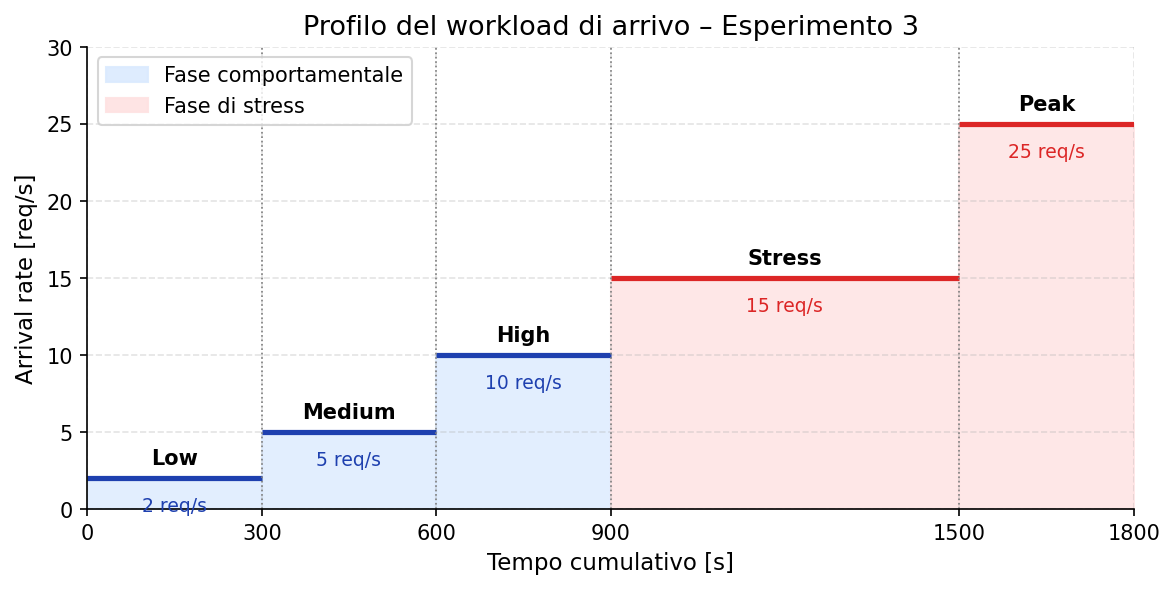
\includegraphics[width=0.95\textwidth]{figures/validation/exp3/01-wokload.png}
    \caption{Profilo del workload di arrivo nel Run~B. Le prime tre fasi
             (\emph{Low}, \emph{Medium}, \emph{High}) sono identiche al
             Run~A; le ultime due (\emph{Stress} e \emph{Peak}) inducono
             condizioni di saturazione progressiva. Il tasso configurato è
             mantenuto costante da k6 tramite l'esecutore
             \texttt{constant-arrival-rate}.}
    \label{fig:exp3-workload-profile}
\end{figure}

Il workload non è mono-funzione né mono-zona: cinque funzioni diverse
e cinque zone geografiche sono distribuite in modo bilanciato tra le
richieste, come mostrato nella Figura~\ref{fig:exp3-workload-mix}.
Questa eterogeneità è necessaria per valutare lo scheduler in
condizioni rappresentative di un deployment reale, in cui il nodo serve
funzioni con profili energetici molto diversi e riceve segnali di CI
da zone con caratteristiche elettriche differenti.

\begin{figure}[H]
    \centering
    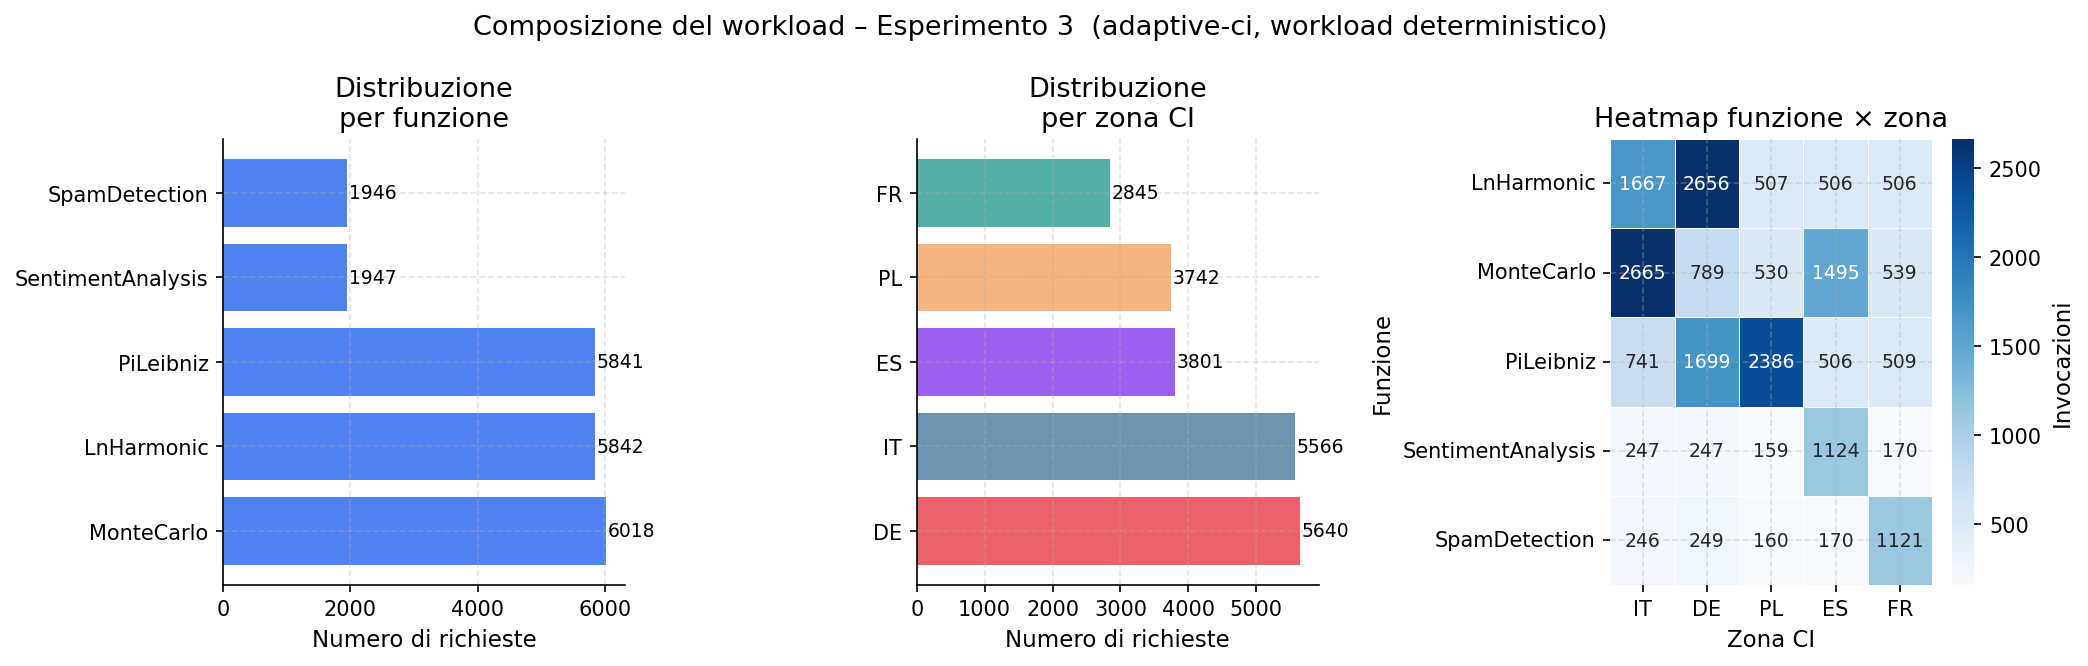
\includegraphics[width=0.98\textwidth]{figures/validation/exp3/09_workload_mix_function_zone.png}
    \caption{Composizione del workload nel Run~B: distribuzione per
             funzione invocata (sinistra), per zona CI (centro) e
             heatmap funzione~$\times$~zona (destra). La sequenza è
             deterministica e identica per tutte e tre le policy.}
    \label{fig:exp3-workload-mix}
\end{figure}

\subsubsection{Risultati}
\label{subsubsec:esperimento3-parte2-risultati}

\paragraph{Latenza e saturazione della coda.}
La Figura~\ref{fig:exp3-latency-decomp} mostra la latenza mediana
disaggregata nelle due componenti --- attesa in coda e durata di
esecuzione --- per fase e policy. La scala logaritmica sull'asse
verticale permette di confrontare contemporaneamente valori che
differiscono di quattro ordini di grandezza.

\begin{figure}[H]
    \centering
    \includegraphics[width=0.98\textwidth]{figures/validation/exp3/02_latency_decomposition_log.pdf}
    \caption{Decomposizione della latenza mediana per fase e policy
             (scala logaritmica). La parte tratteggiata rappresenta
             l'attesa in coda (p50); la parte piena la durata di
             esecuzione (p50). Le barre con pattern a croce indicano
             fasi in cui $\lambda{=}1$ non ha completato alcuna
             richiesta: il riferimento è il timeout di k6 (180~s).
             $\lambda{=}0$ rimane stabile sotto i 5~ms in tutte le fasi;
             \emph{adaptive-ci} cresce gradualmente con il carico;
             $\lambda{=}1$ accumula code di oltre 100~s già dalla fase
             \emph{Medium}.}
    \label{fig:exp3-latency-decomp}
\end{figure}

Per $\lambda{=}1$ il collo di bottiglia non è nella logica
dello scheduler, ma nell'accumulo di richieste in coda. Questo
distingue il fenomeno osservato da una degradazione delle prestazioni di
esecuzione: il sistema è corretto nel \emph{cosa} esegue, ma non riesce
a sostenere il ritmo con cui le richieste arrivano.

\paragraph{Throughput effettivo.}
La Figura~\ref{fig:exp3-throughput} confronta il throughput effettivo
--- richieste completate con HTTP~200 per secondo --- con il tasso
configurato da k6.

\begin{figure}[H]
    \centering
    \includegraphics[width=0.90\textwidth]{figures/validation/exp3/03-throughput.png}
    \caption{Throughput effettivo vs arrival rate configurato per fase e
             policy. $\lambda{=}0$ e \emph{adaptive-ci} seguono il
             profilo configurato in tutte le fasi; $\lambda{=}1$ inizia
             a divergere dalla fase \emph{Medium} e collassa nelle fasi
             di stress.}
    \label{fig:exp3-throughput}
\end{figure}

\paragraph{Frazione cumulativa di completamento.}
La Figura~\ref{fig:exp3-completion} introduce una rappresentazione
alternativa alla CDF classica del tempo di risposta. L'asse verticale
riporta la percentuale di richieste completate \emph{sul totale
inviato}, non sul sottoinsieme delle sole richieste andate a buon fine.
Questa scelta evita una distorsione tipica dei sistemi sotto stress: una
CDF calcolata solo sui completamenti di $\lambda{=}1$ restituirebbe una
distribuzione apparentemente normale, ma taciterebbe il fatto che il
96.5\% delle richieste inviate non ha mai ricevuto risposta. -(da rivedere)

\begin{figure}[H]
    \centering
    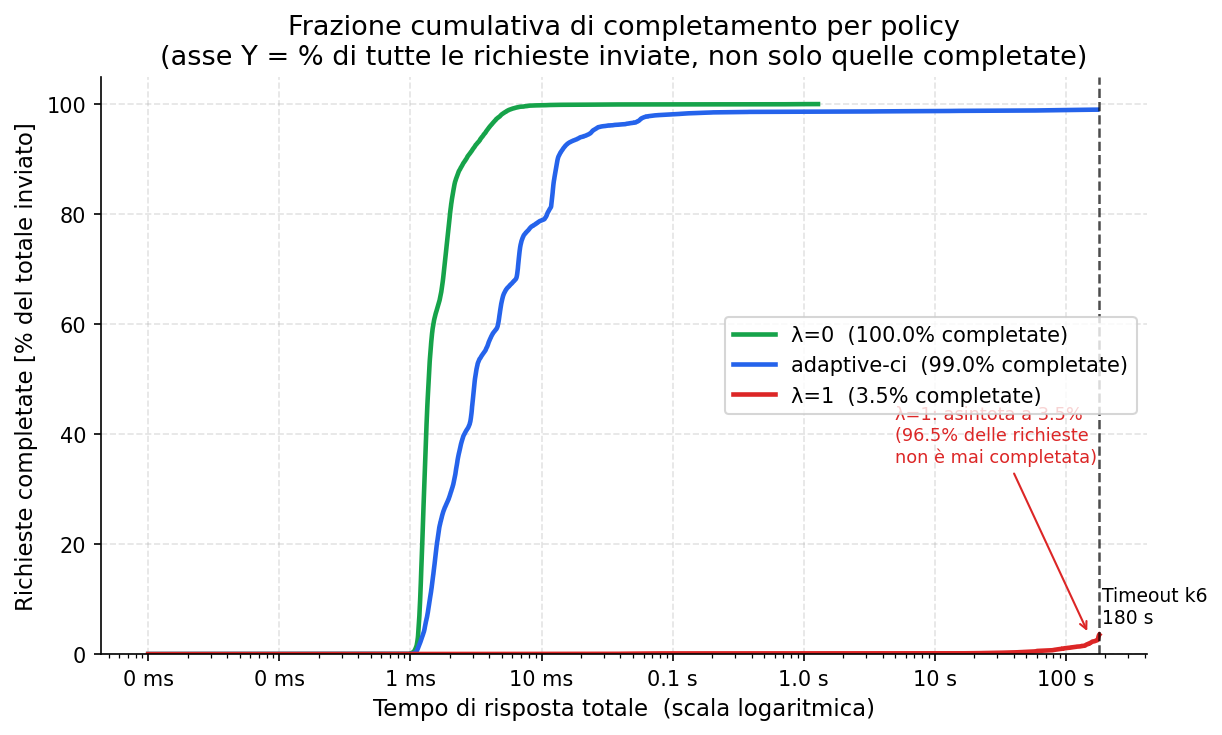
\includegraphics[width=0.90\textwidth]{figures/validation/exp3/05_completion_fraction.png}
    \caption{Frazione cumulativa di completamento per policy (scala
             logaritmica sull'asse $x$). L'asse $y$ indica la
             percentuale di richieste completate rispetto al totale
             inviato. Le curve di $\lambda{=}0$ e \emph{adaptive-ci}
             raggiungono il 100\% e il 99\% entro pochi secondi;
             la curva di $\lambda{=}1$ asintota al 3.5\%, mostrando
             che il 96.5\% delle richieste non ha mai ricevuto risposta
             entro il timeout di 180~s.}
    \label{fig:exp3-completion}
\end{figure}

\paragraph{Confronto quantitativo per fase.}
La Figura~\ref{fig:exp3-phase-table} riassume, per ciascuna
combinazione di fase e policy, le metriche operative principali:
tasso di completamento, throughput, percentili di durata e di coda.
Le celle evidenziate in verde indicano il valore migliore per quella
fase; quelle in rosso il peggiore.

\begin{figure}[H]
    \centering
    \includegraphics[width=0.98\textwidth]{figures/validation/exp3/06_comparison_table_phase_policy.png}
    \caption{Confronto operativo per fase e policy. Nelle fasi
             \emph{Low} e \emph{Medium} le tre policy sono comparabili;
             la differenziazione emerge progressivamente con il crescere
             del carico. $\lambda{=}1$ mostra le prime code misurabili
             già in \emph{Medium}; in \emph{High} e \emph{Stress} il
             completamento scende a zero. \emph{adaptive-ci} mantiene
             metriche paragonabili a $\lambda{=}0$ fino a \emph{Stress},
             con un primo degrado visibile solo nel \emph{Peak}.}
    \label{fig:exp3-phase-table}
\end{figure}

\subsubsection{Distribuzione delle varianti selezionate}
\label{subsubsec:esperimento3-parte2-varianti}

La Figura~\ref{fig:exp3-variant-dist} mostra la distribuzione
percentuale delle varianti selezionate dalla policy \emph{adaptive-ci}
per ciascuna funzione, aggregata sull'intero Run~B. Questa figura serve
a verificare che lo scheduler non collassi su una scelta fissa sotto
carico, ma continui a modulare la selezione in funzione del segnale
di carbon intensity ricevuto.

\begin{figure}[H]
    \centering
    \includegraphics[width=0.98\textwidth]{figures/validation/exp3/08_variant_distribution_by_function.png}
    \caption{Distribuzione percentuale delle varianti selezionate da
             \emph{adaptive-ci} per funzione nel Run~B. L'ordine va
             dalla variante meno costosa (sinistra) a quella più costosa
             (destra). Le varianti agli estremi della frontiera di Pareto
             compaiono con frequenza residua: lo scheduler occupa la
             regione intermedia del trade-off, con una distribuzione
             coerente con i valori medi di CI campionati nelle diverse
             fasi orarie.}
    \label{fig:exp3-variant-dist}
\end{figure}

La distribuzione conferma un comportamento già osservato negli
Esperimenti~1 e~2: le varianti agli estremi --- quella a minima energia
e quella a massima qualità --- compaiono solo nei momenti in cui la CI
è sistematicamente molto bassa o molto alta rispetto alla storia della
zona. La grande maggioranza delle invocazioni ricade su varianti
intermedie, con pesi che variano tra le funzioni in funzione della
struttura della loro frontiera di Pareto. Questo segnala che lo
scheduler non è disturbato dalla concorrenza delle richieste: il piano
di controllo legge il segnale ambientale in modo stabile e lo traduce
in scelte coerenti anche sotto carico.

\subsection{Interpretazione}
\label{subsec:esperimento3-interpretazione}

I risultati dell'Esperimento~3 completano la valutazione dello scheduler
carbon-aware lungo una dimensione che gli Esperimenti~1 e~2 non
affrontano: la coesistenza tra la logica di selezione della variante e
un flusso di richieste concorrente.

\paragraph{Coerenza del comportamento carbon-aware sotto carico.}
Il Run~A mostra che, in assenza di saturazione, il confronto
energetico e qualitativo tra le policy replica il pattern degli
esperimenti precedenti. La variabilità del tasso di arrivo tra le fasi
non influenza le scelte dello scheduler: la distribuzione delle varianti
varia in funzione della CI campionata, non del numero di richieste
concorrenti. Il tempo di risposta riflette il peso computazionale della
variante selezionata, confermando che il piano di controllo non
introduce overhead misurabile nel percorso critico dell'invocazione.

\paragraph{Stabilità di $\lambda{=}0$ e \emph{adaptive-ci}.}
Nel Run~B, $\lambda{=}0$ completa il 100\% delle richieste in tutte le
fasi, con latenza stabile nell'ordine del millisecondo. Questo risultato
è strutturale: le varianti leggere selezionate da questa policy hanno
tempi di esecuzione contenuti che permettono al nodo di servire flussi
intensi senza accumulare code. \emph{Adaptive-ci} completa il 99\% delle
richieste sull'intero workload; i fallimenti si concentrano nella sola
fase \emph{Peak} (25~req/s) e corrispondono a timeout dovuti a code che
si formano sotto il carico massimo, non a errori di configurazione
(HTTP~422 è sempre zero per tutte le policy).

\paragraph{Saturazione di $\lambda{=}1$ e sua causa.}
La policy a massima qualità è la più instabile dal punto di vista
operativo. Già dalla fase \emph{Medium} (5~req/s) si accumulano code
con p50 superiore a 100~secondi; nelle fasi \emph{High} e \emph{Stress}
nessuna richiesta viene completata. Questo collasso non è causato da
errori logici o di configurazione: è la conseguenza diretta della
scelta sistematica di varianti computazionalmente costose, che riduce
la capacità del nodo di servire il flusso in arrivo.

Il caso $\lambda{=}1$ costituisce un risultato di interesse autonomo:
mostra che il costo operativo di una strategia di scheduling non può
essere valutato indipendentemente dal profilo di carico a cui il sistema
è soggetto. Una policy che privilegia sempre la qualità può essere
sostenibile a basso traffico, ma produce instabilità a carichi medi o
elevati. Lo scheduler carbon-aware, selezionando dinamicamente la
variante in funzione della CI, evita questo problema nei regimi di
carico testati: nelle fasi di alta CI sceglie varianti più leggere,
riducendo il carico computazionale sul nodo proprio nei momenti in cui
il flusso di richieste è tipicamente più intenso.

% -----------------------------------------------------------
\section{Discussione generale}
\label{sec:discussione-generale}
% -----------------------------------------------------------

I tre esperimenti rispondono a domande complementari. I primi due
confrontano due modi diversi di interpretare il segnale di carbon
intensity. La calibrazione europea dell'Esperimento~1 fornisce una scala
comune: è utile per confrontare zone diverse senza introdurre soglie
specifiche per ciascuna rete e per osservare come la stessa politica si
comporta al variare del mix elettrico. La calibrazione locale
dell'Esperimento~2 è invece più vicina a un deployment reale: il valore di
$\lambda$ riflette quanto la CI corrente sia alta o bassa rispetto alla
storia della zona, evitando che una soglia europea unica produca decisioni
non proporzionate in reti strutturalmente molto diverse.

In entrambi i casi lo scheduler occupa una posizione intermedia tra
\emph{always-accurate}, che preserva la qualità ignorando il costo
ambientale, e \emph{always-energy}, che minimizza il consumo ignorando la
qualità. Il terzo esperimento verifica infine che questa selezione possa
essere eseguita anche in presenza di carico variabile, senza introdurre un
overhead tale da compromettere la latenza del servizio.

\paragraph{Limitazioni.}
I risultati evidenziano alcune limitazioni del sistema proposto. La prima
riguarda le zone con CI prossima al punto medio della sigmoide: in tali
condizioni, piccole variazioni della CI possono attraversare soglie di
selezione e produrre cambi più frequenti di variante. La seconda riguarda
le funzioni con frontiera di Pareto poco estesa: quando sono disponibili
solo pochi punti non dominati, lo scheduler ha meno possibilità di
modulare gradualmente il compromesso e i salti di qualità possono essere
più marcati. La terza riguarda i burst molto intensi: il sistema resta
vincolato alla capacità del piano di controllo, alla latenza di
\texttt{etcd} e alla frequenza con cui le metriche energetiche vengono
aggiornate.

\paragraph{Sintesi.}
Nel complesso, la valutazione mostra che l'estensione proposta consente di
collocare Serverledge tra due estremi operativi ben definiti:
\emph{always-accurate}, che massimizza la qualità ignorando il costo
ambientale, e \emph{always-energy}, che minimizza il consumo ignorando la
qualità. Lo scheduler carbon-aware occupa una regione intermedia e
variabile dello spazio di trade-off, determinata dalla carbon intensity
della zona e vincolata al consenso esplicito dell'utente. La riduzione
delle emissioni non è ottenuta tramite una degradazione indiscriminata,
ma attraverso una scelta contestuale e misurabile lungo la frontiera di
Pareto, coerente con il segnale ambientale osservato a runtime.
